\documentclass[journal]{IEEEtran}
\IEEEoverridecommandlockouts
%%%%%%%%%%%%%%%%%%%%%%%%%%%%%%%%%%%%%%
%%%%%%%% PRINCIPALES PAQUETES %%%%%%%%
%%%%%%%%%%%%%%%%%%%%%%%%%%%%%%%%%%%%%%
\usepackage{fancyhdr}
\usepackage{graphicx}
\usepackage[spanish,es-tabla,es-noshorthands]{babel}
\usepackage[utf8]{inputenc}
\usepackage[T1]{fontenc}
\DeclareFontShape{T1}{ptm}{m}{scit}{<->ssub * ptm/m/it}{}
\DeclareFontShape{T1}{ptm}{b}{scit}{<->ssub * ptm/b/it}{}
\DeclareFontShape{T1}{ptm}{bx}{scit}{<->ssub * ptm/b/it}{}
\usepackage{wrapfig}
\usepackage{array}
\usepackage{multirow}
\usepackage{adjustbox}
\usepackage{nccmath}
%\usepackage{anysize}
\usepackage{subfigure}
\usepackage{amsmath,amssymb,amsthm,mathtools,bm,amsfonts,latexsym} % para tener disponibilidad de diversos simbolos
\usepackage{enumerate}
\usepackage{enumitem}
\usepackage{booktabs}
\usepackage{float}
\usepackage{threeparttable}
\usepackage{colortbl}
\usepackage{ifpdf}
\usepackage{rotating}
\usepackage{cite}
\usepackage{stfloats}
\usepackage{url}
\usepackage{tabularx}
\usepackage{listings}
\usepackage[hidelinks,hypertexnames=false]{hyperref}
\mathtoolsset{showonlyrefs}
%%%%%%%%%%%%%%%%%%%%%%%%%%%%%%%%%%%%%%%%%%%
%%% CREAR Y REESCRIBIR ALGUNOS COMANDOS %%%
%%%%%%%%%%%%%%%%%%%%%%%%%%%%%%%%%%%%%%%%%%%
\newcolumntype{P}[1]{>{\centering\arraybackslash}p{#1}}  %% Se crea un nuevo tipo de columna llamada P.
\newcolumntype{L}[1]{>{\raggedright\arraybackslash}p{#1}}
\newcommand{\tabitem}{~~\llap{\textbullet}~~}
\newcommand{\ctt}{\centering\scriptsize\textbf} %%\ctt abrevia el comando \centering\scriptsize\textbf
\newcommand{\dtt}{\scriptsize\textbf} %%\dtt abrevia el comando \scriptsize\textbf
\renewcommand\IEEEkeywordsname{Palabras clave}
%%%%%%%%%%%%%%%%%%%%%%%%%%%%%%%%%%%%%%%%%%%
\setlength{\headheight}{14pt}
\hypersetup{pdfauthor={OpenAI},pdftitle={Reporte: función descriptiva, continuación numérica y atractores ocultos fraccionarios}}
\raggedbottom

\newtheorem{theorem}{Teorema}[section]
\newtheorem{remark}[theorem]{Observación}
\newtheorem{proposition}[theorem]{Proposición}
\newtheorem{definition}[theorem]{Definición}

\newcommand{\CaputoD}[1]{{}^{C}D_t^{#1}}
\newcommand{\CaputoDz}[2]{{}^{C}D_{#2}^{#1}}
\newcommand{\WeylD}[1]{{}^{LW}D_t^{#1}}
\newcommand{\WeylDz}[2]{{}^{LW}D_{#2}^{#1}}
\newcommand{\R}{\mathbb{R}}
\newcommand{\C}{\mathbb{C}}
\newcommand{\figplaceholder}[2]{%
\begin{figure}[H]
\centering
\fbox{\parbox[c][#1][c]{\dimexpr\columnwidth-2\fboxsep-2\fboxrule\relax}{\centering\itshape Inserte aquí la gráfica indicada.}}
\caption{#2}
\end{figure}}
\newcommand{\importantbox}[1]{%
\begin{center}
\fbox{\parbox{0.93\textwidth}{#1}}
\end{center}}


\DeclareMathOperator*{\di}{\mathrm{d}\!}
\DeclareMathOperator{\sgn}{sgn}
\def\at{
  \left.
  \vphantom{\int}
  \right|
}

% correct bad hyphenation here
\hyphenation{op-tical net-works semi-conduc-tor} %% Con este comando se especifican como pueden seprarse las sílabas adecuadamente en caso una palabra quede en dos lineas diferentes de texto

\graphicspath{{Figs/}{chua_integer_runs/balanced/final_pdf_figs/}}  %%Ruta donde se encuentran las imágenes, que esté vacio indica que las imagenes están dentro de la misma carpeta que contiene el archivo .tex


%%%%%%%%%%%%%%%%%%%%%%%%%%%%%%%%%%%%%%%%%%%%%%%%%%%%%%%%%%
%%% ENCABEZADO DE LAS PÁGINAS TIPO UNICAFAM %%%%%%%%%%%%%%
%%%%%%%%%%%%%%%%%%%%%%%%%%%%%%%%%%%%%%%%%%%%%%%%%%%%%%%%%%
\newcommand{\MYhead}{\smash{\scriptsize
\hfil\parbox[t][\height][t]{\textwidth}{\centering
\begin{picture}(0,0) \put(-40,-19){\IfFileExists{inaoe.png}{
\includegraphics[width=12mm]{inaoe.png}}{}} \end{picture} \hspace{4.8cm}
Sistemas dinámicos de orden fraccionario \hspace{3.55cm} DEE6073: SDOF\\
 \hspace{4cm} Tarea 1. Métodos numéricos para derivadas fraccionarias \hspace{3cm} Periodo 2023-I \\  \hspace{13.3cm} Depto. de Electrónica
% \\  \hspace{6.8cm} María Fernanda Moreno López\hspace{3.3cm} Prof.: Dr. Oscar Martínez-Fuentes\\
\underline{\hspace{ \textwidth}}}\hfil\hbox{}}}
\makeatletter
% normal pages
\def\ps@headings{%
\def\@oddhead{\MYhead}%
\def\@evenhead{\MYhead}}%
% title page
\def\ps@IEEEtitlepagestyle{%
\def\@oddhead{\MYhead}%
\def\@evenhead{\MYhead}}%
\makeatother
% make changes take effect
\pagestyle{headings}
% adjust as needed
\addtolength{\footskip}{0\baselineskip}
\addtolength{\textheight}{-1\baselineskip}
%%%%%%%%%%%%%%%%%%%%%%%%%%%%%%%%%%%%%%%%%%%%%%%%%%%%%%%%%%
%%%%%%%%%%%%%%%%%%%%%%%%%%%%%%%%
%%%%% INICIO DEL DOCUMENTO %%%%%
%%%%%%%%%%%%%%%%%%%%%%%%%%%%%%%%
\begin{document}
%%%%%%%%%%%%%%%%%%%%%%%%%%%%
%%% TÍTULO DEL DOCUMENTO %%%
%%%%%%%%%%%%%%%%%%%%%%%%%%%%
\title{Localización de atractores ocultos en sistemas caóticos de orden fraccionario mediante función descriptiva y continuación numérica}
%%%%%%%%%%%%%%%%%%%%%%%%%%%%
%%%%%%%%% AUTORES %%%%%%%%%
%%%%%%%%%%%%%%%%%%%%%%%%%%%
\author{María Fernanda Moreno-López}% stops a space

%%%%%%%%%%%%%%%%%%%%%%%%%%%

% Comando que indica la generación del título
\maketitle

%%%%%%%%%%%%%%%%%%%%%%%%%%%%%%%%%%%%%
%%% PRIMERA SECCIÓN DEL DOCUMENTO %%%
%%%%%%%%%%%%%%%%%%%%%%%%%%%%%%%%%%%%%


\newpage

\section{Introducción}
La localización de atractores ocultos en sistemas caóticos de orden fraccionario requiere una reformulación conceptual más cuidadosa que en el caso entero. Para sistemas con derivada de Caputo de orden conmensurado \(q\in(0,1)\), el operador dinámico incorpora memoria, la estabilidad lineal se expresa mediante funciones de Mittag--Leffler y, además, no existen en general soluciones periódicas exactas no constantes en sistemas autónomos invariantes en el tiempo de tipo Caputo \cite{TavazoeiHaeri2009,AreaLosadaNieto2014}. Por esta razón, no resulta apropiado trasladar directamente al caso fraccionario el análisis del caso entero. 

El documento se organiza del siguiente modo: primero se resume el caso entero como referencia metodológica. Después se desarrolla el marco fraccionario, incluyendo la justificación de la linealización, la ausencia general de periodicidad exacta en Caputo, el papel del problema auxiliar de Weyl y el puente Weyl--Caputo. A continuación se formula el procedimiento operativo para el caso fraccionario, se presentan dos ejemplos de estudio: el sistema de Chua no suave y el sistema de Chua suave con no linealidad \(\arctan\).

\section{Estrategia metodológica}
La estrategia metodológica se resume en la cadena
\[
\begin{aligned}
&\text{separación tipo Lur'e} + \text{función descriptiva} + \text{Nyquist}\\
&\Longrightarrow\; \text{predictor armónico}\\
&\Longrightarrow\; \text{construcción de semilla}\\
&\Longrightarrow\; \text{continuación numérica}\\
&\Longrightarrow\; \text{verificación de ocultedad y validación dinámica}.
\end{aligned}
\]

El papel de cada bloque puede resumirse en los siguientes pasos:

%¿Qué es un Modo?: Es la respuesta del sistema asociada a un par de polos (valores propios) específico. Cada polo representa una frecuencia natural y amortiguamiento.Dominancia: Los modos "dominantes" son aquellos que tardan más en extinguirse (es decir, los más cercanos al eje imaginario en el plano \(s\)). Estos dictan el comportamiento transitorio principal del sistema, como el tiempo de establecimiento o el sobrepaso.Subespacio: Se refiere al plano formado por los vectores propios (eigenvectores) correspondientes a estos modos dominantes. Al analizar el sistema dentro de este subespacio, se ignora el comportamiento de modos rápidos o de alta frecuencia, simplificando el diseño del controlador.Aplicación: Es fundamental para modelar sistemas de alto orden, permitiendo a los ingenieros diseñar controladores efectivos al enfocarse en las partes más lentas y críticas de la dinámica.En resumen, es descomponer la dinámica del sistema y quedarse solo con los componentes lentos o "dominantes" para facilitar su análisis y control.

\begin{enumerate}
    \item \textbf{Separación tipo Lur'e.} El sistema se reescribe aislando un bloque lineal y una no linealidad escalar estática. 
    
    \begin{equation}
        x = Ax + B\varphi (Cx) := F_{Lur'e}(x)
    \end{equation}
    
    Esta separación permite definir una función de transferencia y una función descriptiva del primer armónico.

    \item \textbf{Predictor armónico.} Se obtienen una frecuencia base \(\omega_0\), una ganancia equivalente \(k\) y una amplitud candidata \(a_0\) a partir de una condición de cierre armónico del tipo
    \[
    1 + N(a)\,W_q(i\omega)=0.
    \]
    Este resultado se interpreta como predictor del régimen estacionario del sistema real.

    \item \textbf{Construcción de semilla.} Con \((\omega_0,k,a_0)\) se construye una condición inicial asociada al subespacio modal dominante\footnote{El subespacio modal dominante hace referencia a una simplificación de orden reducido de un sistema complejo, enfocándose únicamente en los modos que tienen mayor impacto en la respuesta dinámica general.} del sistema lineal modificado.

    \item \textbf{Continuación numérica.} Se introduce una familia homotópica en la no linealidad,
    \[
    {}^{C}D_t^q \bm{x}=P_0\bm{x}+\varepsilon\,\bm{q}\,\delta(r^\top \bm{x}),
    \qquad \varepsilon\in[0,1],
    \]
    y se transporta la semilla desde un problema auxiliar hasta el sistema original.

    \item \textbf{Verificación de ocultedad.} El régimen final sólo se clasifica como atractor oculto si no es excitado desde vecindades de los equilibrios.
\end{enumerate}

\section{Caso de referencia en orden entero}

Este caso de referencia permite identificar con claridad el papel de la separación tipo Lur'e, el cierre armónico, la construcción de la semilla y la continuación numérica, que después serán reinterpretados al caso fraccionario.

\subsection{Sistema de Chua de orden entero}
\noindent El circuito de Chua con no linealidad PWL se escribe como

\begin{equation}
    \label{eq:chua}
    \begin{aligned}
        \dot{x} &= \alpha \left( y - x - f(x) \right), \\
        \dot{y} &= x - y + z, \\
        \dot{z} &= -(\beta y + \gamma z),
    \end{aligned}
\end{equation}

\noindent donde el término no lineal se suele modelar por
\begin{equation*}
f(x)=m_1x+\frac{1}{2}(m_0-m_1)\big(|x+1|-|x-1|\big),
\end{equation*}

\noindent que equivale a

\begin{equation*}
    f(x) = m_1 x + (m_0-m_1)sat(x), 
\end{equation*}
donde 


\begin{equation}\label{eq:sat_chua}
    sat(x) = \begin{cases}
    -1 & \text{si } x < -1, \\
    x & \text{si } |x| \leq 1, \\
    1 & \text{si } x > 1.
\end{cases}
\end{equation}

\noindent Se define la parte no lineal pura como
\begin{equation}\label{eq:psi_chua_def}
  \psi(x) \coloneqq \frac{1}{2}(m_0-m_1)\big(|x+1|-|x-1|\big).
\end{equation}

\noindent de modo que $f(x)=m_1x+\psi(x)$.

\noindent Considérese $X=\begin{bmatrix}x&y&z\end{bmatrix}^\mathsf{T}\in\mathbb{R}^3$.
Al sustituir $f(x)=m_1x+\psi(x)$ en \eqref{eq:chua}:
\[
\begin{aligned}
\dot x &= \alpha\Big(y-x-m_1x-\psi(x)\Big)\\
       &= -\alpha(m_1+1)x+\alpha y-\alpha\,\psi(x).
\end{aligned}
\]
De este modo, \eqref{eq:chua} puede reescribirse como
\begin{equation}\label{eq:lure}
\dot X = PX + q\,\psi(r^\mathsf{T}X),
\end{equation}
con
\begin{equation}\label{eq:Pqr}
\begin{aligned}
P&=
\begin{bmatrix}
-\alpha(m_1+1) & \alpha & 0\\
1 & -1 & 1\\
0 & -\beta & -\gamma
\end{bmatrix},\\
q&=
\begin{bmatrix}
-\alpha\\0\\0
\end{bmatrix},\qquad
r=
\begin{bmatrix}
1\\0\\0
\end{bmatrix},\qquad
r^\mathsf{T}X=x.
\end{aligned}
\end{equation}

\noindent Para el sistema \eqref{eq:lure}, la función de transferencia se define como
\begin{equation}\label{eq:Wdef}
W(p)=r^\mathsf{T}(P-pI)^{-1}q.
\end{equation}
En esta expresión, $p\in\mathbb{C}$ e $I$ denota la matriz identidad $3\times3$.

\noindent Dado que $r=e_1$ y $q=-\alpha e_1$, se obtiene
\[
W(p)=-\alpha\,(P-pI)^{-1}_{11}.
\]
El cofactor $(1,1)$ viene dado por el determinante del menor
\[
\det\begin{bmatrix}
-1-p & 1\\
-\beta & -\gamma-p
\end{bmatrix}
=(p+1)(p+\gamma)+\beta.
\]
En consecuencia,
\begin{equation}\label{eq:Wexplicit}
W(p)= -\alpha\,\frac{(p+1)(p+\gamma)+\beta}{\det(P-pI)}.
\end{equation}
Además,
\[
\det(P-pI)=\big(-\alpha(m_1+1)-p\big)\big((p+1)(p+\gamma)+\beta\big)
+\alpha(p+\gamma).
\]
%(Se obtiene expandiendo por la primera fila.)

\noindent Se busca un par $(\omega_0,k)$ tal que:
\begin{align}
\Im W(i\omega_0)&=0,\qquad \omega_0>0, \label{eq:condIm}\\
k&=-\frac{1}{\Re W(i\omega_0)}.\label{eq:condk}
\end{align}

La ganancia equivalente \(k\) se incorpora en la parte lineal que se usará como punto de partida para construir la semilla inicial.

\noindent Poniendo $p=i\omega$ y definiendo
\begin{equation}\label{eq:Np}
  N(p)\coloneqq (p+1)(p+\gamma)+\beta.
\end{equation}
Con $\omega\in\mathbb{R}$:
\[
N(i\omega)=N_r+iN_i,\quad N_r=\beta+\gamma-\omega^2,\quad N_i=\omega(1+\gamma).
\]

Al escribir el denominador de \eqref{eq:Wexplicit} como
\[
D(i\omega)=D_r+iD_i,
\]
la condición \eqref{eq:condIm} equivale a imponer que la parte imaginaria del cociente $N(i\omega)/D(i\omega)$ se anule:

\begin{equation}
\begin{aligned}
W(i\omega)
&=-\alpha\,\frac{N_r+iN_i}{D_r+iD_i}\\
&=-\alpha\,\frac{(N_rD_r+N_iD_i)+i(N_iD_r-N_rD_i)}{D_r^2+D_i^2}.
\end{aligned}
\end{equation}

Por tanto,
\begin{equation}
\Im\{W(i\omega)\}=0
\iff N_iD_r-N_rD_i=0.
\end{equation}

De esta condición se obtiene la ecuación equivalente \eqref{eq:omegaeq}.

\begin{equation}\label{eq:omegaeq}
(\beta+\gamma-\omega^2)^2
-\alpha(\beta+\gamma-\omega^2)
+(1+\gamma)^2\omega^2
+\alpha\gamma(1+\gamma)=0.
\end{equation}

\noindent La ecuación \eqref{eq:omegaeq} puede tener más de una raíz positiva. La frecuencia que se emplea para construir la semilla debe satisfacer condiciones adicionales de admisibilidad de la linealización armónica\cite{GuanXie2025,KuznetsovEtAl2017}. Se construye la matriz lineal modificada
\begin{equation}\label{eq:P0}
P_0=P+kqr^\mathsf{T}.
\end{equation}
La frecuencia seleccionada debe hacer que \(P_0\) tenga dos autovalores
puramente imaginarios y un tercer autovalor real negativo:
\[
\sigma(P_0)=\{\,i\omega_0,\,-i\omega_0,\,-d\,\},
\qquad d>0.
\]

Esta condición significa que la parte lineal modificada contiene una
componente oscilatoria con frecuencia \(\omega_0\), mientras que la tercera dirección decae\footnote{El \emph{modo transversal} es la dirección restante del sistema lineal modificado, asociada al autovalor \(-d\). Se llama transversal porque no pertenece al plano oscilatorio generado por \(\pm i\omega_0\).}. Por ello, la trayectoria inicial puede construirse a partir de una oscilación dominante. Además, la frecuencia candidata debe ser compatible con la amplitud
predicha por la función descriptiva. En particular, debe existir una amplitud \(a_0\) dentro de la región considerada de la no linealidad, en este caso \(a_0\geq 1\), tal que
\[
\Phi(a_0)=0.
\]
Finalmente, se verifica la condición
\[
b_1\left.\frac{d\Phi}{da}\right|_{a=a_0}<0.
\]
Esta desigualdad indica que la solución aproximada obtenida para el sistema derivado es localmente estable dentro de la aproximación por función descriptiva \cite{GuanXie2025,KuznetsovEtAl2017}.

\noindent Sustituyendo los parámetros usados en \cite{Danca2017}:
\[
\begin{aligned}
\alpha&=8.4562,\quad \beta=12.0732,\quad \gamma=0.0052,\\
m_0&=-0.1768,\quad m_1=-1.1468,
\end{aligned}
\]
la rama que satisface las condiciones anteriores es
\[
\omega_0\approx 2.0392.
\]
Al sustituir este valor en \eqref{eq:condk}, se obtiene
\[
k\approx 0.2098.
\]
Posteriormente, al resolver la ecuación de balance armónico
\(\Phi(a)=0\), se obtiene
\[
a_0\approx 5.8576.
\]

\noindent Dado que $qr^\mathsf{T}$ de \eqref{eq:P0} sólo afecta la entrada $(1,1)$ de la matriz $P$, se obtiene
\begin{equation}\label{eq:P0_matrix}
  P_0=
\begin{bmatrix}
-\alpha(m_1+1+k) & \alpha & 0\\
1 & -1 & 1\\
0 & -\beta & -\gamma
\end{bmatrix}.
\end{equation}
Se consideran los sistemas derivados de la forma
\begin{equation}\label{eq:derived}
\dot X = P_0X + q\,\varepsilon\,\varphi(r^\mathsf{T}X),
\end{equation}
donde $\varepsilon\in[0,1]$ es pequeño al inicio y
\begin{equation}\label{eq:varphi_residual}
\varphi(\sigma)=\psi(\sigma)-k\sigma.
\end{equation}
Para \(\varepsilon=0\), el sistema derivado se reduce al sistema lineal
modificado y la solución esperada permanece cercana a la oscilación armónica inicial. 
\[
\dot X=P_0X,
\]

Al aumentar \(\varepsilon\), se incorpora gradualmente la
parte no lineal residual \(\varphi(r^\mathsf{T}X)\). \(\varepsilon\) se incrementa
hasta \(1\) mediante continuación numérica, usando en cada paso la solución
del valor anterior como condición inicial para el siguiente. En particular, cuando
\(\varepsilon=1\), se recupera el sistema objetivo\cite{GuanXie2025,KuznetsovEtAl2017}:

\begin{equation}
\begin{aligned}
\dot X
&=P_0X+q\,\varphi(r^\mathsf{T}X)\\
&=\bigl(P+kqr^\mathsf{T}\bigr)X
  +q\Bigl(\psi(r^\mathsf{T}X)-k\,r^\mathsf{T}X\Bigr)\\
&=PX+kq\,r^\mathsf{T}X
  +q\psi(r^\mathsf{T}X)-kq\,r^\mathsf{T}X\\
&=PX+q\psi(r^\mathsf{T}X).
\end{aligned}
\end{equation}
\noindent Se busca una transformación lineal no singular \(X=SY\)\footnote{La no singularidad de \(S\) indica que tiene inversa \(S^{-1}\) y que \(\det(S)\neq 0\), esto garantiza que el cambio de variables es invertible y que \(Y=S^{-1}X\).} que permita escribir el sistema derivado en coordenadas donde la oscilación armónica asociada a \(\omega_0\) aparezca explícitamente. Por ello, \eqref{eq:derived} se lleva a la forma
\begin{equation}\label{eq:canon}
\dot Y = AY + b\,\varepsilon\,\varphi(c^\mathsf{T}Y),
\end{equation}
donde
\[
A=
\begin{bmatrix}
0 & -\omega_0 & 0\\
\omega_0 & 0 & 0\\
0 & 0 & -d
\end{bmatrix},
\qquad
b=\begin{bmatrix}b_1\\ b_2\\ 1\end{bmatrix},
\qquad
c=\begin{bmatrix}1\\0\\-h\end{bmatrix}.
\]
Esta forma facilita construir una condición inicial armónica en las coordenadas \(Y\), que después se transforma a las coordenadas originales mediante \(X(0)=SY(0)\).

\noindent Para obtener las relaciones entre ambas representaciones, se sustituye
\(X=SY\) en \eqref{eq:derived}. Como \(S\) es constante,
\[
\dot X=S\dot Y.
\]
Entonces
\[
S\dot Y=P_0SY+q\,\varepsilon\,\varphi(r^\mathsf{T}SY).
\]
Multiplicando por \(S^{-1}\), se obtiene
\[
\dot Y
=
S^{-1}P_0S\,Y
+
S^{-1}q\,\varepsilon\,
\varphi(r^\mathsf{T}SY).
\]
Al comparar esta ecuación con \eqref{eq:canon}, se concluye que deben
cumplirse las condiciones
\begin{equation}\label{eq:relS}
A=S^{-1}P_0S,\qquad
b=S^{-1}q,\qquad
c^\mathsf{T}=r^\mathsf{T}S.
\end{equation}
Estas igualdades se llaman condiciones de consistencia porque garantizan
que \eqref{eq:canon} no es un sistema diferente, sino el mismo sistema
derivado escrito en las coordenadas \(Y\).

\noindent La función de transferencia en la forma canónica se obtiene a partir
del sistema escrito en las coordenadas \(Y\). Si \(u=\varepsilon
\varphi(c^\mathsf{T}Y)\) se interpreta como la entrada al bloque lineal y
\(\sigma=c^\mathsf{T}Y\) como la salida, entonces
\[
W_A(p)=c^\mathsf{T}(A-pI)^{-1}b.
\]
Esta función es equivalente a la función de transferencia del sistema
modificado en las coordenadas originales,
\begin{equation}
  W_0(p)=r^\mathsf{T}(P_0-pI)^{-1}q,
  \label{eq:W0_modificado}
\end{equation}
porque las condiciones de consistencia \eqref{eq:relS} implican
\[
\begin{aligned}
W_A(p)
&=c^\mathsf{T}(A-pI)^{-1}b\\
&=r^\mathsf{T}S\left(S^{-1}(P_0-pI)S\right)^{-1}S^{-1}q\\
&=r^\mathsf{T}S\left(S^{-1}(P_0-pI)^{-1}S\right)S^{-1}q\\
&=r^\mathsf{T}(P_0-pI)^{-1}q\\
&=W_0(p).
\end{aligned}
\]
Por tanto, puede calcularse la transferencia usando la forma canónica sin
modificar la relación entrada--salida del sistema.

\noindent Ahora, como
\[
A-pI=
\begin{bmatrix}
-p & -\omega_0 & 0\\
\omega_0 & -p & 0\\
0 & 0 & -d-p
\end{bmatrix},
\]
se tiene
\[
(A-pI)^{-1}
=
\begin{bmatrix}
\dfrac{-p}{p^2+\omega_0^2} &
\dfrac{\omega_0}{p^2+\omega_0^2} &
0\\[2mm]
\dfrac{-\omega_0}{p^2+\omega_0^2} &
\dfrac{-p}{p^2+\omega_0^2} &
0\\[2mm]
0&0&-\dfrac{1}{p+d}
\end{bmatrix}.
\]
Multiplicando por \(b\),
\[
(A-pI)^{-1}b
=
\begin{bmatrix}
\dfrac{-b_1p+b_2\omega_0}{p^2+\omega_0^2}\\[2mm]
\dfrac{-b_1\omega_0-b_2p}{p^2+\omega_0^2}\\[2mm]
-\dfrac{1}{p+d}
\end{bmatrix}.
\]
Finalmente,
\[
\begin{aligned}
W_A(p)
&=c^\mathsf{T}(A-pI)^{-1}b\\
&=
\begin{bmatrix}
1&0&-h
\end{bmatrix}
\begin{bmatrix}
\dfrac{-b_1p+b_2\omega_0}{p^2+\omega_0^2}\\[2mm]
\dfrac{-b_1\omega_0-b_2p}{p^2+\omega_0^2}\\[2mm]
-\dfrac{1}{p+d}
\end{bmatrix}\\
&=
\frac{-b_1p+b_2\omega_0}{p^2+\omega_0^2}
+\frac{h}{p+d}.
\end{aligned}
\]
\noindent Por lo que, la forma canónica induce la función de transferencia
\begin{equation}\label{eq:WA}
W_A(p)=c^\mathsf{T}(A-pI)^{-1}b
=\frac{-b_1p+b_2\omega_0}{p^2+\omega_0^2}+\frac{h}{p+d}.
\end{equation}
\noindent Para obtener \(d\) y \(k\), se impone que la matriz lineal modificada \(P_0\) tenga el espectro requerido por la construcción
armónica. A partir de \eqref{eq:P0_matrix}, se calcula el polinomio
característico usando
\[
\det(P_0-pI).
\]
Introduciendo
\[
B\coloneqq \alpha(m_1+1+k),
\]
la matriz \(P_0-pI\) queda escrita como
\[
P_0-pI=
\begin{bmatrix}
-B-p & \alpha & 0\\
1 & -1-p & 1\\
0 & -\beta & -\gamma-p
\end{bmatrix}.
\]
y su determinante,
\begin{equation}
\begin{aligned}
\det(P_0-pI)
&=
-p^3-(B+1+\gamma)p^2\\
&\quad
-\bigl[(\beta+\gamma)+B(1+\gamma)-\alpha\bigr]p\\
&\quad
-B(\beta+\gamma)+\alpha\gamma .
\end{aligned}
\label{eq:detP0B}
\end{equation}

\noindent La construcción armónica exige que \(P_0\) tenga los autovalores
\[
p=\pm i\omega_0,\qquad p=-d,
\]
entonces, el polinomio característico debe ser

\begin{eqnarray}
(i\omega_0-p)(-i \omega_0 -p)(-d-p)=-(p+d)(p^2+\omega_0^2)\\
=-p^3-dp^2-\omega_0^2p-d\omega_0^2.
\label{eq:detObj}
\end{eqnarray}

\noindent Igualando los coeficientes de \eqref{eq:detP0B} y \eqref{eq:detObj}, se obtiene primero que el coeficiente de \(p^3\) coincide directamente. Los coeficientes de \(p^2\) y \(p\) dan

\begin{align}
d&=B+1+\gamma, \label{eq:dB}\\
\omega_0^2&=(\beta+\gamma)+B(1+\gamma)-\alpha. \label{eq:wB}
\end{align}
De \eqref{eq:wB} se despeja
\[
B=
\frac{\omega_0^2-\beta-\gamma+\alpha}{1+\gamma}.
\]
Sustituyendo este valor en \eqref{eq:dB}, se obtiene
\begin{equation}
d=
\frac{\alpha+\omega_0^2-\beta+1+\gamma+\gamma^2}{1+\gamma}.
\end{equation}

Además, como
\[
B=\alpha(m_1+1+k),
\]
se tiene
\[
k=\frac{B}{\alpha}-m_1-1.
\]
Finalmente,
\begin{equation}
k=
\frac{-\alpha\bigl(m_1+m_1\gamma+\gamma\bigr)
+\omega_0^2-\gamma-\beta}{\alpha(1+\gamma)}.
\end{equation}

\noindent Al igualar los términos independientes de \eqref{eq:detP0B} y \eqref{eq:detObj}, se obtiene
\[
-B(\beta+\gamma)+\alpha\gamma=-d\omega_0^2.
\]
Equivalentemente,
\[
R(\omega_0)
\coloneqq
-B(\beta+\gamma)+\alpha\gamma+d\omega_0^2=0.
\]
Esta expresión  es la parte que queda después de haber usado los coeficientes de \(p^2\) y \(p\) para determinar \(d\) y \(B\).

Al sustituir las expresiones ya obtenidas para \(B\) y \(d\), se obtiene
\begin{equation}
\begin{aligned}
R(\omega_0)
&=
\frac{1}{1+\gamma}
\Big[
(\beta+\gamma-\omega_0^2)^2
-\alpha(\beta+\gamma-\omega_0^2)
\\
&\qquad
+(1+\gamma)^2\omega_0^2
+\alpha\gamma(1+\gamma)
\Big].
\end{aligned}
\end{equation}
Como \(\gamma>0\), se tiene \(1+\gamma\neq 0\). La expresión
\[
R(\omega_0)=0
\]
si y sólo si
\begin{equation}
(\beta+\gamma-\omega_0^2)^2
-\alpha(\beta+\gamma-\omega_0^2)
+(1+\gamma)^2\omega_0^2
+\alpha\gamma(1+\gamma)=0.
\end{equation}

\noindent Su papel es verificar que la frecuencia \(\omega_0\)
seleccionada satisface la ecuación de frecuencia obtenida previamente. Si \(R(\omega_0)=0\), entonces el polinomio característico de \(P_0\) coincide completamente con \eqref{eq:detObj}. Si \(R(\omega_0)\neq 0\), entonces la frecuencia elegida no es compatible
con esa asignación espectral.
\noindent Ahora se determinan \(h,b_1,b_2\). A partir de \eqref{eq:W0_modificado}, \eqref{eq:detObj} y del numerador de \eqref{eq:Wexplicit}, se obtiene
\begin{equation}
W_0(p)=\frac{\alpha N(p)}{(p+d)(p^2+\omega_0^2)}.
\end{equation}
Como \(W_0(p)=W_A(p)\). Usando \eqref{eq:WA} y multiplicando por el denominador común \((p+d)(p^2+\omega_0^2)\), resulta
\begin{equation}
\alpha N(p)
=
(-b_1p+b_2\omega_0)(p+d)+h(p^2+\omega_0^2).
\end{equation}
Al sustituir el numerador de \eqref{eq:Wexplicit} en esta identidad, expandir el lado derecho y comparar coeficientes, se obtiene
\begin{align}
(-b_1p+b_2\omega_0)(p+d)+h(p^2+\omega_0^2)
&=(-b_1+h)p^2\\
&\quad +(-b_1d+b_2\omega_0)p\\
&\quad +(b_2\omega_0 d+h\omega_0^2).
\end{align}
\begin{align}
-b_1+h&=\alpha, \label{eq:coef2}\\
-b_1d+b_2\omega_0&=\alpha(1+\gamma), \label{eq:coef1}\\
b_2\omega_0 d+h\omega_0^2&=\alpha(\beta+\gamma). \label{eq:coef0}
\end{align}

De \eqref{eq:coef2},
\[
b_1=h-\alpha.
\]
Sustituyendo en \eqref{eq:coef1},
\[
-(h-\alpha)d+b_2\omega_0=\alpha(1+\gamma),
\]
por lo que
\begin{equation}
b_2\omega_0=\alpha(1+\gamma-d)+hd. \label{eq:b2omega}
\end{equation}
Sustituyendo \eqref{eq:b2omega} en \eqref{eq:coef0},
\[
d\bigl[\alpha(1+\gamma-d)+hd\bigr]+h\omega_0^2
=
\alpha(\beta+\gamma).
\]
Agrupando los términos con \(h\),
\[
h(d^2+\omega_0^2)
=
\alpha\bigl[\beta+\gamma-(1+\gamma)d+d^2\bigr].
\]
Así,
\begin{equation}
h=
\frac{\alpha\bigl(\gamma+\beta-(1+\gamma)d+d^2\bigr)}
{\omega_0^2+d^2}.
\end{equation}

Como \(b_1=h-\alpha\), se obtiene
\begin{align}
b_1
&=
\frac{\alpha\bigl(\gamma+\beta-(1+\gamma)d+d^2\bigr)}
{\omega_0^2+d^2}
-\alpha\\
&=
\frac{\alpha\bigl(\gamma+\beta-\omega_0^2-(1+\gamma)d\bigr)}
{\omega_0^2+d^2}.
\end{align}
Finalmente, usando \eqref{eq:b2omega},
\[
b_2=\frac{\alpha(1+\gamma-d)+hd}{\omega_0}.
\]
Al sustituir la expresión de \(h\),
\begin{equation}
b_2=
\frac{\alpha\bigl((1+\gamma-d)\omega_0^2+(\gamma+\beta)d\bigr)}
{\omega_0(\omega_0^2+d^2)}.
\end{equation}

Con los parámetros del ejemplo, se obtiene:
\[
\begin{aligned}
d&\approx 1.5385,\quad h\approx 16.7158,\\
b_1&\approx 8.2596,\quad b_2\approx 10.4001.
\end{aligned}
\]

\noindent Al resolver \eqref{eq:relS}, se obtiene una matriz $S$ particular:
\[
S=
\begin{bmatrix}
s_{11} & s_{12} & s_{13}\\
s_{21} & s_{22} & s_{23}\\
s_{31} & s_{32} & s_{33}
\end{bmatrix},
\]
con
\begin{equation*}
\begin{aligned}
s_{11} &= 1,\\
s_{12} &= 0,\\
s_{13} &= -h,\\
s_{21} &= m_1+1+k,\\
s_{22} &= -\frac{\omega_0}{\alpha},\\
s_{23} &= -\frac{h}{\alpha}\bigl(\alpha(m_1+1+k)-d\bigr),\\
s_{31} &= \frac{\alpha(m_1+k)-\omega_0^2}{\alpha},\\
s_{32} &= -\frac{1}{\alpha\omega_0}\Bigl(\alpha(\beta+\gamma)(m_1+k)+\alpha\beta-\gamma\omega_0^2\Bigr),\\
s_{33} &= \frac{h}{\alpha}\bigl(\alpha(m_1+k)(d-1)+d(1+\alpha-d)\bigr).
\end{aligned}
\end{equation*}

Una vez construida la matriz lineal modificada \(P_0\), la no linealidad se
separa como
\[
\psi(\sigma)=k\sigma+\varphi(\sigma),
\]
donde \(\varphi\) está definida en \eqref{eq:varphi_residual}.
La ganancia \(k\) representa la parte lineal equivalente que se incorporó en
\(P_0\). Por tanto, \(\varphi\) es la no linealidad residual que todavía debe
ser compensada por el balance armónico.

El método de función descriptiva aproxima la respuesta de una no linealidad
estática ante una entrada sinusoidal conservando únicamente su primer
armónico. En este caso se considera
\[
\sigma(t)=a\sin\theta,\qquad \theta=\omega_0 t,
\]
y se calcula el primer armónico de \(\varphi(a\sin\theta)\). Como la
saturación de Chua es impar, su componente fundamental queda en fase con
\(\sin\theta\). Por ello, basta calcular la amplitud del armónico senoidal.

Para la no linealidad de Chua definida en \eqref{eq:psi_chua_def}, con la saturación dada por \eqref{eq:sat_chua}, se trabaja con la rama \(a\ge 1\), porque en esa región la señal \(a\sin\theta\) alcanza la zona de saturación.

Sea
\[
\theta_0=\arcsin\frac{1}{a}.
\]
Entonces, en el primer cuadrante,
\[
\operatorname{sat}(a\sin\theta)=
\begin{cases}
a\sin\theta, & 0\le \theta\le \theta_0,\\[1ex]
1, & \theta_0\le \theta\le \dfrac{\pi}{2}.
\end{cases}
\]
Por simetría impar, la amplitud del primer armónico de
\(\psi(a\sin\theta)\) es
\[
B_\psi(a)
=
\frac{4}{\pi}(m_0-m_1)
\left[
\int_0^{\theta_0}a\sin^2\theta\,d\theta
+
\int_{\theta_0}^{\pi/2}\sin\theta\,d\theta
\right].
\]

Las integrales se calculan como
\[
\int_0^{\theta_0}\sin^2\theta\,d\theta
=
\frac{\theta_0}{2}
-
\frac{\sin(2\theta_0)}{4},
\]
y
\[
\int_{\theta_0}^{\pi/2}\sin\theta\,d\theta
=
\cos\theta_0.
\]
Como
\[
\sin\theta_0=\frac{1}{a},
\qquad
\cos\theta_0=
\sqrt{1-\frac{1}{a^2}},
\]
se tiene
\[
\sin(2\theta_0)
=
2\sin\theta_0\cos\theta_0
=
\frac{2}{a}\sqrt{1-\frac{1}{a^2}}.
\]
Por tanto,
\[
\int_0^{\theta_0}a\sin^2\theta\,d\theta
=
\frac{a\theta_0}{2}
-
\frac{1}{2}\sqrt{1-\frac{1}{a^2}},
\]
mientras que
\[
\int_{\theta_0}^{\pi/2}\sin\theta\,d\theta
=
\sqrt{1-\frac{1}{a^2}}.
\]
Al sumar,
\[
\int_0^{\theta_0}a\sin^2\theta\,d\theta
+
\int_{\theta_0}^{\pi/2}\sin\theta\,d\theta
=
\frac{a\theta_0}{2}
+
\frac{1}{2}\sqrt{1-\frac{1}{a^2}}.
\]
Así,
\[
B_\psi(a)
=
\frac{2}{\pi}(m_0-m_1)
\left(
a\theta_0+
\sqrt{1-\frac{1}{a^2}}
\right).
\]
Sustituyendo \(\theta_0=\arcsin(1/a)\),
\[
B_\psi(a)
=
\frac{2}{\pi}(m_0-m_1)
\left(
a\arcsin\frac{1}{a}
+
\sqrt{1-\frac{1}{a^2}}
\right).
\]
Usando
\[
\arcsin x=\frac{\pi}{2}-\arccos x,
\]
queda
\[
B_\psi(a)
=
\frac{2}{\pi}(m_0-m_1)
\left(
\frac{\pi a}{2}
+
\sqrt{1-\frac{1}{a^2}}
-
a\arccos\frac{1}{a}
\right).
\]

Ahora se considera la parte residual definida en \eqref{eq:varphi_residual}.
Si \(\sigma=a\sin\theta\), el primer armónico de \(k\sigma\) tiene amplitud
\(ka\). Por tanto, la amplitud del primer armónico residual es
\[
B_\varphi(a)=B_\psi(a)-ka.
\]
El balance armónico exige que este primer armónico residual se anule:
\[
B_\varphi(a)=0.
\]
Multiplicando por \(\pi\), se define la función escalar
\[
\Phi(a)=\pi B_\varphi(a).
\]
Por tanto,
\begin{equation}\label{eq:Phi}
\Phi(a)=0,
\end{equation}
donde
\[
\Phi(a)=
2(m_0-m_1)
\left(
\frac{\pi a}{2}
+
\sqrt{1-\frac{1}{a^2}}
-
a\arccos\frac{1}{a}
\right)
-\pi ak.
\]

La ecuación \(\Phi(a)=0\) determina la amplitud candidata \(a_0\) de la
oscilación dominante. Esta amplitud no se obtiene de una simulación directa
del sistema no lineal completo, sino de la aproximación armónica de la
no linealidad residual.

Para analizar la admisibilidad local de esta solución aproximada, se calcula
la derivada de \(\Phi\). Sea
\[
g(a)=
\frac{\pi a}{2}
+
\sqrt{1-\frac{1}{a^2}}
-
a\arccos\frac{1}{a}.
\]
Entonces
\[
\Phi(a)=2(m_0-m_1)g(a)-\pi ak.
\]
Derivando,
\[
\frac{d}{da}
\sqrt{1-\frac{1}{a^2}}
=
\frac{1}{a^3\sqrt{1-\frac{1}{a^2}}},
\]
y
\[
\frac{d}{da}
\left(
a\arccos\frac{1}{a}
\right)
=
\arccos\frac{1}{a}
+
\frac{1}{a\sqrt{1-\frac{1}{a^2}}}.
\]
Por tanto,
\[
g'(a)
=
\frac{\pi}{2}
+
\frac{1}{a^3\sqrt{1-\frac{1}{a^2}}}
-
\arccos\frac{1}{a}
-
\frac{1}{a\sqrt{1-\frac{1}{a^2}}}.
\]
Los términos con radical se simplifican como
\[
\frac{1}{a^3\sqrt{1-\frac{1}{a^2}}}
-
\frac{1}{a\sqrt{1-\frac{1}{a^2}}}
=
-\frac{1}{a}\sqrt{1-\frac{1}{a^2}},
\]
de modo que
\[
g'(a)
=
\frac{\pi}{2}
-
\frac{1}{a}\sqrt{1-\frac{1}{a^2}}
-
\arccos\frac{1}{a}.
\]
Finalmente,
\[
\frac{d\Phi}{da}
=
2(m_0-m_1)
\left(
\frac{\pi}{2}
-
\frac{1}{a}\sqrt{1-\frac{1}{a^2}}
-
\arccos\frac{1}{a}
\right)
-\pi k.
\]

La raíz \(a_0\) de \(\Phi(a)=0\), con \(a_0\ge 1\), se usa para construir una
condición inicial compatible con el modo oscilatorio dominante de la forma
canónica. En particular, se fija la condición inicial
\begin{equation}\label{eq:Y0}
Y(0)=
\begin{pmatrix}
a_0\\
0\\
0
\end{pmatrix}.
\end{equation}
Luego, se regresa a las coordenadas originales mediante
\begin{equation}\label{eq:X0_from_Y}
X(0)=SY(0).
\end{equation}
La derivada \(\Phi'(a_0)\) se utiliza en la condición
\[
b_1\Phi'(a_0)<0,
\]
que indica estabilidad local dentro de la aproximación por función descriptiva. Esta condición no demuestra por sí sola la existencia ni la ocultedad del atractor; sólo valida la semilla armónica usada para iniciar la continuación numérica.

\noindent Se resuelve \eqref{eq:Phi} para $a\ge 1$. Con los parámetros del ejemplo, se reporta una amplitud inicial
\[
a_0\approx 5.8576,
\]
la cual satisface las condiciones requeridas por el teorema usado en el artículo (existencia de una solución periódica estable para el primer sistema derivado con $\varepsilon$ pequeño).

\noindent Se selecciona la condición inicial en el espacio $Y$ dada por \eqref{eq:Y0}. Entonces, al evaluar \eqref{eq:X0_from_Y}, se obtiene
\begin{equation}\label{eq:x0}
X(0)=
\begin{bmatrix}
a_0 s_{11}\\ a_0 s_{21}\\ a_0 s_{31}
\end{bmatrix}
=
\begin{bmatrix}
a_0\\
a_0(m_1+1+k)\\
a_0\big(\alpha(m_1+k)-\omega_0^2\big)/\alpha
\end{bmatrix}.
\end{equation}
Con $\omega_0=2.0392$, $k=0.2098$ y $a_0=5.8576$:
\[
\begin{aligned}
x(0)&\approx 5.8576,\\
y(0)&\approx 0.3694,\\
z(0)&\approx -8.3686.
\end{aligned}
\]

\subsection{Resultados numéricos del caso entero}

Se evaluó el sistema de Chua de orden entero con parámetros
\[
\begin{aligned}
\alpha &= 8.45620, & \beta &= 12.07320,\\
\gamma &= 0.00520, & m_0 &= -0.17680,\\
m_1 &= -1.14680.
\end{aligned}
\]
La integración numérica se realizó con esquema operativo EFORK-3 evaluado
en \(q=1\).

La reescritura tipo Lur'e
\[
\dot X=PX+q_v\psi(r^\mathsf{T}X),
\qquad
\sigma=r^\mathsf{T}X,
\]
se verificó con error nulo,
\[
\|PX+q_v\psi-F(X)\|=0.
\]
Por tanto, la separación entre el bloque lineal y la no linealidad escalar es
consistente con la implementación usada para construir la función de
transferencia y aplicar la función descriptiva.

La condición de Nyquist asociada al cierre armónico produjo dos ramas
candidatas:
\[
\begin{aligned}
(\omega_1,k_1) &= (2.03919,0.20987),\\
(\omega_2,k_2) &= (3.24529,0.95969).
\end{aligned}
\]
Se seleccionó la primera rama,
\[
\omega_0=2.03919,
\qquad
k=0.20987.
\]
Al resolver la ecuación de balance armónico \(\Phi(a)=0\), se obtuvo
\[
a_0=5.85615,
\qquad
\Phi(a_0)\approx -1.27500\times10^{-16}.
\]
La condición inicial inducida por la transformación canónica fue
\[
X_0=
\begin{pmatrix}
5.85615\\
0.36933\\
-8.36654
\end{pmatrix}.
\]

La matriz lineal modificada \(P_0=P+kq_vr^\mathsf{T}\) resultó
\[
P_0=
\begin{pmatrix}
-0.53331 & 8.45620 & 0.\\
1. & -1. & 1.\\
0. & -12.07320 & -0.00520
\end{pmatrix}.
\]
Sus autovalores fueron
\[
\lambda_1=-1.53851,
\qquad
\lambda_{2,3}\approx \pm 2.03919\,i.
\]
Por tanto, el modo transversal es
\[
d=1.53851.
\]
Los parámetros canónicos obtenidos de la equivalencia de funciones de
transferencia fueron
\[
h=16.71582,
\qquad
b_1=8.25962,
\qquad
b_2=10.40007.
\]
La equivalencia entre la transferencia original modificada y la transferencia
canónica se verificó con error
\[
\operatorname{err}_{W}=4.72100\times10^{-15}.
\]

A partir de la semilla \(X_0\), se aplicó continuación numérica mediante
\(\varepsilon\in[0,1]\). Para \(\varepsilon=0\), el sistema corresponde al
problema auxiliar linealizado por la ganancia equivalente \(k\). Para
\(\varepsilon=1\), se recupera el sistema no lineal original. Al finalizar la
continuación se obtuvo
\[
X_{\varepsilon=1}=
\begin{pmatrix}
1.99297\\
1.26397\\
-2.55106
\end{pmatrix}.
\]
Después del transitorio, la trayectoria usada como referencia para el atractor
candidato produjo la semilla efectiva
\[
X_{\mathrm{target}}=
\begin{pmatrix}
4.09187\\
-0.08387\\
-7.50908
\end{pmatrix}.
\]

El análisis espectral de la trayectoria final mostró una frecuencia dominante
en la componente \(x\),
\[
f_d=0.36663\;\mathrm{Hz},
\qquad
\omega_d=2.30358\;\mathrm{rad/s}.
\]
Comparando con la frecuencia predicha por la función descriptiva,
\[
\omega_0=2.03919\;\mathrm{rad/s},
\]
se obtiene el desajuste relativo
\[
\eta=
\frac{|\omega_d-\omega_0|}{\omega_0}
=
0.12966.
\]
La discrepancia es esperable, porque la función descriptiva conserva sólo el
primer armónico de la no linealidad y se usa como generador de semilla, no
como descripción exacta del régimen no lineal completo.

Los exponentes de Lyapunov estimados fueron
\[
(\lambda_1,\lambda_2,\lambda_3)
=
(0.20825,0.01373,-1.36693).
\]
Como \(\lambda_1>0\), la trayectoria localizada presenta evidencia numérica
de sensibilidad a condiciones iniciales. Por tanto, el régimen final es
compatible con dinámica caótica.

Los equilibrios usados en la verificación de ocultedad fueron
\[
E_0=
\begin{pmatrix}
0.\\
0.\\
0.
\end{pmatrix},
\]
\[
E_+=
\begin{pmatrix}
6.58831\\
0.00284\\
-6.58547
\end{pmatrix},
\qquad
E_-=
\begin{pmatrix}
-6.58831\\
-0.00284\\
6.58547
\end{pmatrix}.
\]
Para evaluar la ocultedad se lanzaron trayectorias desde vecindades de estos
equilibrios con radios
\[
\rho\in
\{10^{-5},3\times10^{-5},10^{-4},3\times10^{-4},
10^{-3},3\times10^{-3},10^{-2}\}.
\]
Se usaron \(24\) condiciones iniciales por radio y por equilibrio, por lo que
el número total de pruebas fue
\[
3\times 7\times 24=504.
\]
Los conteos globales fueron
\[
\begin{aligned}
\mathrm{EQ} &= 369, & \mathrm{DIV} &= 69,\\
\mathrm{OTHER} &= 66, & \mathrm{TARGET} &= 0,\\
\mathrm{UNKNOWN} &= 0.
\end{aligned}
\]
El resultado central es
\[
\mathrm{TARGET}=0.
\]
Es decir, ninguna trayectoria iniciada en las vecindades muestreadas de los
equilibrios fue clasificada como perteneciente al atractor objetivo. Por tanto,
el régimen localizado se reporta como un \emph{candidato numérico a atractor
oculto}. La clasificación no debe formularse como demostración global, ya que
la verificación se realizó con un conjunto finito de radios, muestras y tiempos
de integración.

\begin{table*}[htbp]
\centering
\scriptsize
\setlength{\tabcolsep}{3pt}
\renewcommand{\arraystretch}{1.12}
\caption{Resumen de resultados del caso de Chua de orden entero, organizados por procedimiento de obtención.}
\label{tab:chua_integer_results_full}
\begin{adjustbox}{max width=\textwidth}
\begin{tabular}{@{}L{2.7cm}L{3.4cm}L{4.4cm}L{5.8cm}@{}}
\toprule
\textbf{Bloque} &
\textbf{Procedimiento} &
\textbf{Resultado} &
\textbf{Interpretación} \\
\midrule

Parámetros del sistema &
Definición del caso base &
\(\alpha=8.46,\ \beta=12.07,\ \gamma=0.01,\ m_0=-0.18,\ m_1=-1.15\) &
Parámetros usados para la prueba de referencia en orden entero. \\

Orden dinámico &
Configuración del integrador &
\(q=1.00\) &
Caso entero usado como base antes de extender el procedimiento al sistema fraccionario. \\

Forma Lur'e &
Separación algebraica &
\(\|PX+q_v\psi-F(X)\|=0.00\) &
La representación tipo Lur'e reproduce exactamente el campo vectorial implementado. \\

Matriz \(P\) &
Forma Lur'e &
\(\begin{pmatrix}
1.24&8.46&0.00\\
1.00&-1.00&1.00\\
0.00&-12.07&-0.01
\end{pmatrix}\) &
Bloque lineal del sistema separado de la no linealidad escalar. \\

Vectores \(q_v,r\) &
Forma Lur'e &
\(q_v=(-8.46,0.00,0.00)^\mathsf{T}\), \(r=(1.00,0.00,0.00)^\mathsf{T}\) &
La salida escalar de la no linealidad es \(\sigma=r^\mathsf{T}X=x\). \\

Raíces candidatas &
Condición \(\Im W(i\omega)=0\) &
\((\omega,k)=(2.04,0.21),\ (3.25,0.96)\) &
Cruces del diagrama de Nyquist con el eje real. \\

Rama seleccionada &
Nyquist y admisibilidad espectral &
\(\omega_0=2.04,\quad k=0.21\) &
Rama usada para construir \(P_0\) y la semilla armónica. \\

Amplitud armónica &
Balance armónico \(\Phi(a)=0\) &
\(a_0=5.86,\quad \Phi(a_0)\approx -1.28\times10^{-16}\) &
Amplitud compatible con el primer armónico de la no linealidad residual. \\

Cierre armónico &
Función descriptiva y Nyquist &
\(\left|W(i\omega_0)N(a_0)+1\right|=9.93\times10^{-16}\) &
La condición de cierre se satisface con error numérico prácticamente nulo. \\

Matriz \(P_0\) &
Linealización armónica modificada &
\(\begin{pmatrix}
-0.53&8.46&0.00\\
1.00&-1.00&1.00\\
0.00&-12.07&-0.01
\end{pmatrix}\) &
Matriz lineal con ganancia equivalente incorporada. \\

Espectro de \(P_0\) &
Asignación espectral &
\(-1.54,\ \pm 2.04 i\) &
Contiene un plano oscilatorio y un modo transversal estable. \\

Modo transversal &
Coeficientes del polinomio característico &
\(d=1.54\) &
Tasa de decaimiento de la dirección transversal. \\

Parámetros canónicos &
Equivalencia de transferencia &
\(h=16.72,\quad b_1=8.26,\quad b_2=10.40\) &
Parámetros de la forma canónica usada para construir la semilla. \\

Matriz \(S\) &
Transformación \(X=SY\) &
\(\begin{pmatrix}
1.00&0.00&-16.72\\
0.06&-0.24&1.99\\
-1.43&-0.37&15.65
\end{pmatrix}\) &
Transformación no singular hacia coordenadas canónicas. \\

Verificación de \(S\) &
Consistencia algebraica &
\(\|P_0S-SA\|_F=1.80\times10^{-14}\), \(\|Sb-q_v\|=4.08\times10^{-15}\), \(\|rS-c^\mathsf{T}\|=4.14\times10^{-15}\) &
La forma canónica preserva la dinámica entrada--salida del sistema modificado. \\

Error de transferencia &
Comparación \(W_0(p)=W_A(p)\) &
\(4.72\times10^{-15}\) &
La transferencia canónica coincide numéricamente con la transferencia modificada. \\

Semilla inicial &
Transformación \(X_0=S(a_0,0,0)^\mathsf{T}\) &
\(X_0=(5.86,\ 0.37,\ -8.37)\) &
Condición inicial generada por función descriptiva. \\

Estado final de continuación &
Continuación numérica en \(\varepsilon\) &
\(X_{\varepsilon=1}=(1.99,\ 1.26,\ -2.55)\) &
Estado alcanzado al recuperar el sistema no lineal original. \\

Semilla efectiva &
Simulación posterior al transitorio &
\(X_{\mathrm{target}}=(4.09,\ -0.08,\ -7.51)\) &
Punto usado como referencia del atractor candidato. \\

Frecuencia dominante &
FFT de \(x(t)\) &
\(f_d=0.37\ \mathrm{Hz}\), \(\omega_d=2.30\ \mathrm{rad/s}\) &
Frecuencia dominante observada en la salida \(\sigma=x\). \\

Desajuste espectral &
Comparación DF--FFT &
\(\eta=0.13\) &
Diferencia relativa entre la frecuencia predicha por DF y la observada en simulación. \\

Frecuencia PSD &
PSD de Welch &
\(\omega_{\mathrm{PSD}}=2.30\ \mathrm{rad/s}\) &
Confirma la frecuencia dominante observada por FFT. \\

Exponentes de Lyapunov &
Método de Benettin &
\((0.21,\ 0.01,\ -1.37)\) &
Evidencia numérica de caos por \(\lambda_1>0\). \\

Equilibrios &
Resolución algebraica del sistema estacionario &
\(E_0=(0.00,0.00,0.00)\), \(E_+=(6.59,0.00,-6.59)\), \(E_-=(-6.59,0.00,6.59)\) &
Puntos usados para verificar autoexcitación u ocultedad. \\

Sondeos de ocultedad &
Vecindades de equilibrios &
\(504\) pruebas, \(\mathrm{TARGET}=0\) &
No se detectaron trayectorias desde vecindades de equilibrio hacia el atractor objetivo. \\

Conteos globales &
Clasificador de destino &
\(\mathrm{EQ}=369,\ \mathrm{DIV}=69,\ \mathrm{OTHER}=66,\ \mathrm{UNKNOWN}=0\) &
Las trayectorias de prueba convergen a equilibrios, divergen o caen en otros destinos, pero no en el objetivo. \\

Clasificación &
Criterio operacional de cuencas &
Candidato numérico a atractor oculto &
La cuenca del atractor candidato no fue detectada en las vecindades muestreadas de los equilibrios. \\

\bottomrule
\end{tabular}
\end{adjustbox}
\end{table*}

\newpage
\subsection{Figuras}

La Fig.~\ref{fig:chua_int_nyquist} muestra el cierre armónico usado para
seleccionar la rama \((\omega_0,k,a_0)\). La curva \(W(i\omega)\) cruza el eje
real en el punto compatible con \(-1/N(a_0)\), lo que justifica la semilla
inicial usada en la continuación.

\begin{figure}[htbp]
\centering
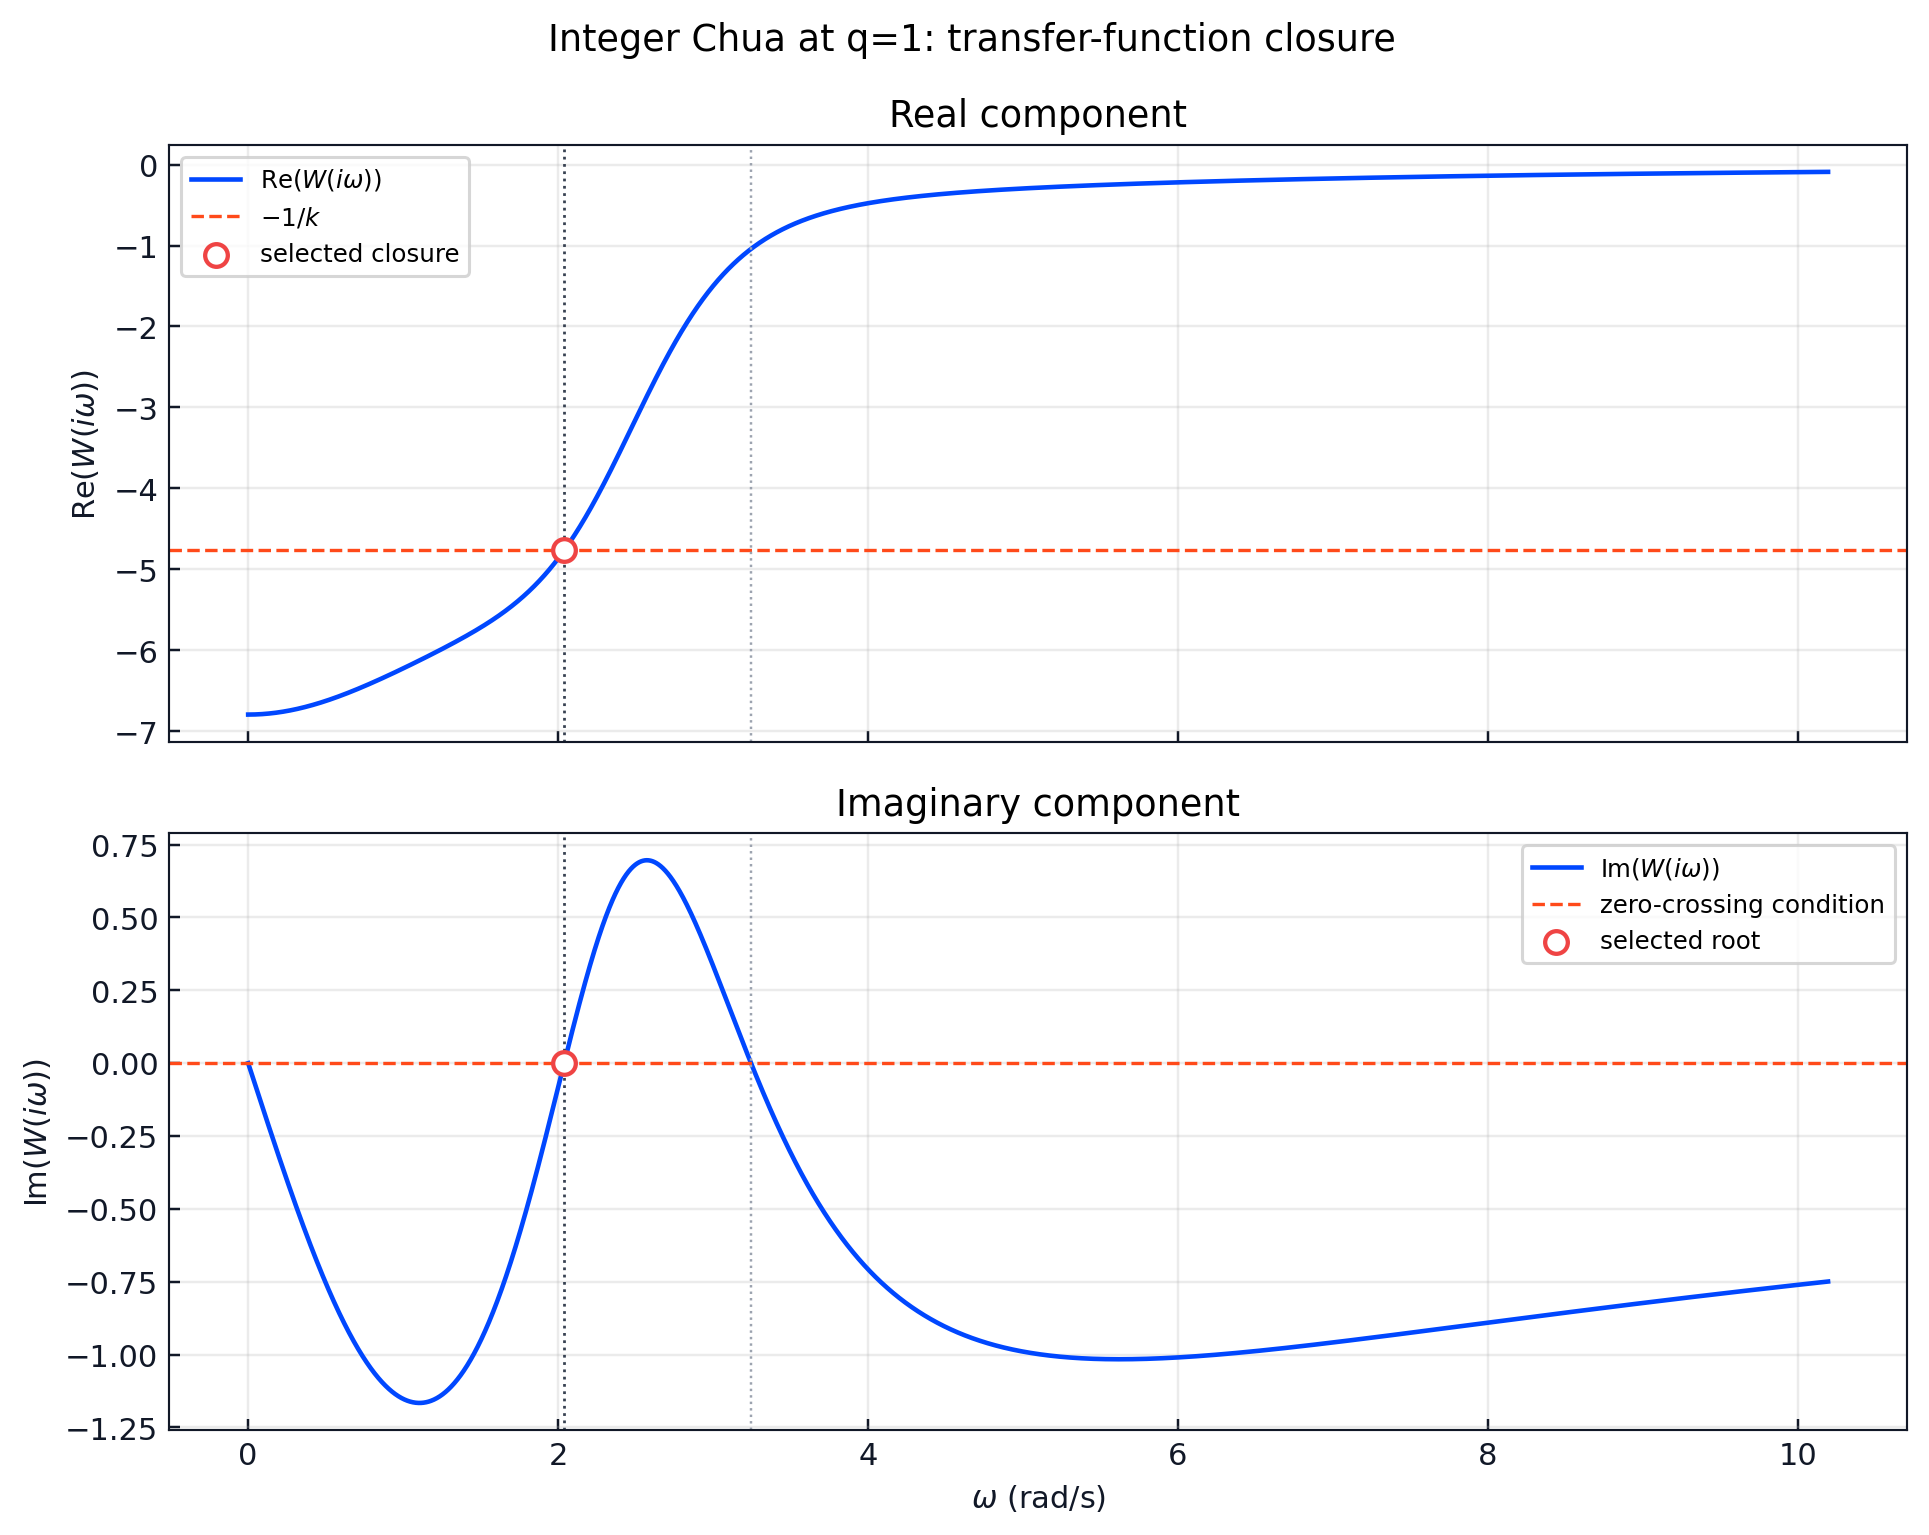
\includegraphics[width=0.82\columnwidth]{fig01c_transfer_real_imag.png}
\caption{Respuesta en frecuencia de la función de transferencia modificada del bloque lineal para el caso entero. Se muestran las partes real e imaginaria de \(W(i\omega)\) en función de la frecuencia \(\omega\), validando el cruce por cero de la parte imaginaria en la frecuencia armónica \(\omega_0\) y el valor correspondiente de la parte real para satisfacer el balance de primer armónico.}
\label{fig:chua_int_nyquist}
\end{figure}

La Fig.~\ref{fig:chua_int_continuation} resume la continuación numérica desde
el sistema derivado hasta el sistema original. La trayectoria de continuación
muestra que la semilla armónica puede transportarse hasta \(\varepsilon=1\),
donde se recupera la no linealidad completa.

\begin{figure}[htbp]
\centering
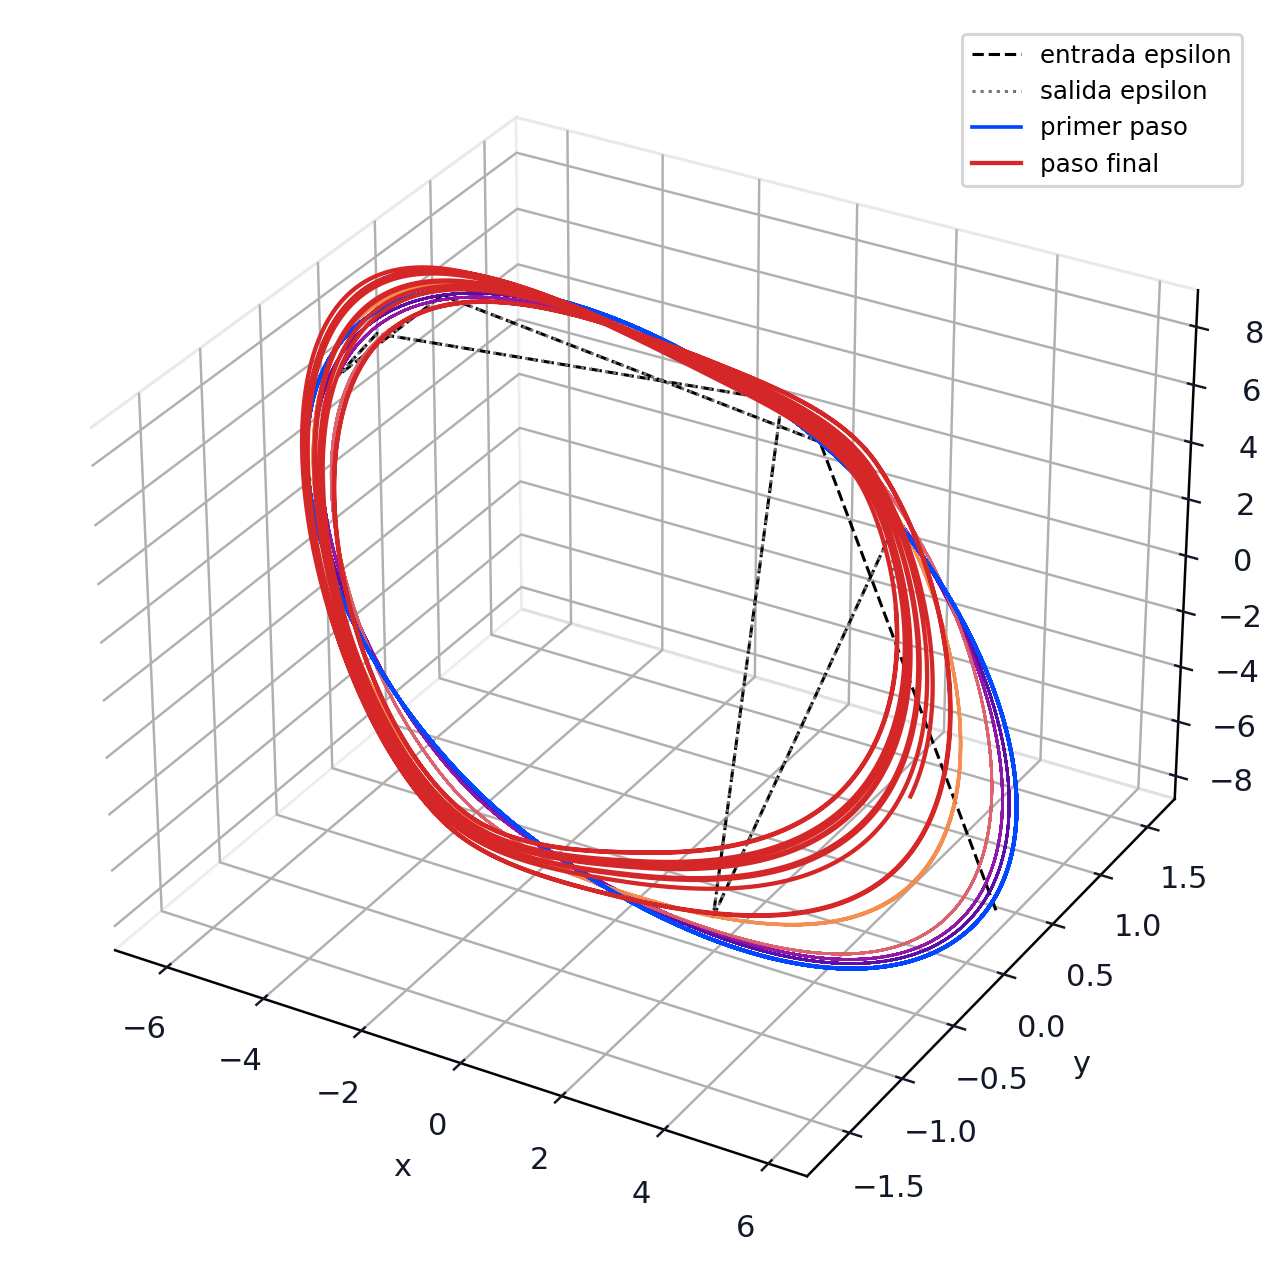
\includegraphics[width=0.82\columnwidth]{fig02d_continuation_story.png}
\caption{Continuación numérica desde el sistema auxiliar hacia el sistema
original. La curva inicial corresponde a la dinámica próxima al predictor
armónico y la curva final al régimen obtenido al completar
\(\varepsilon=1\).}
\label{fig:chua_int_continuation}
\end{figure}

La Fig.~\ref{fig:chua_int_attractor} muestra el régimen final alcanzado tras
la continuación. Los marcadores indican el estado final de la continuación y la
semilla efectiva después del transitorio, usada para caracterizar el atractor
candidato.

\begin{figure}[htbp]
\centering
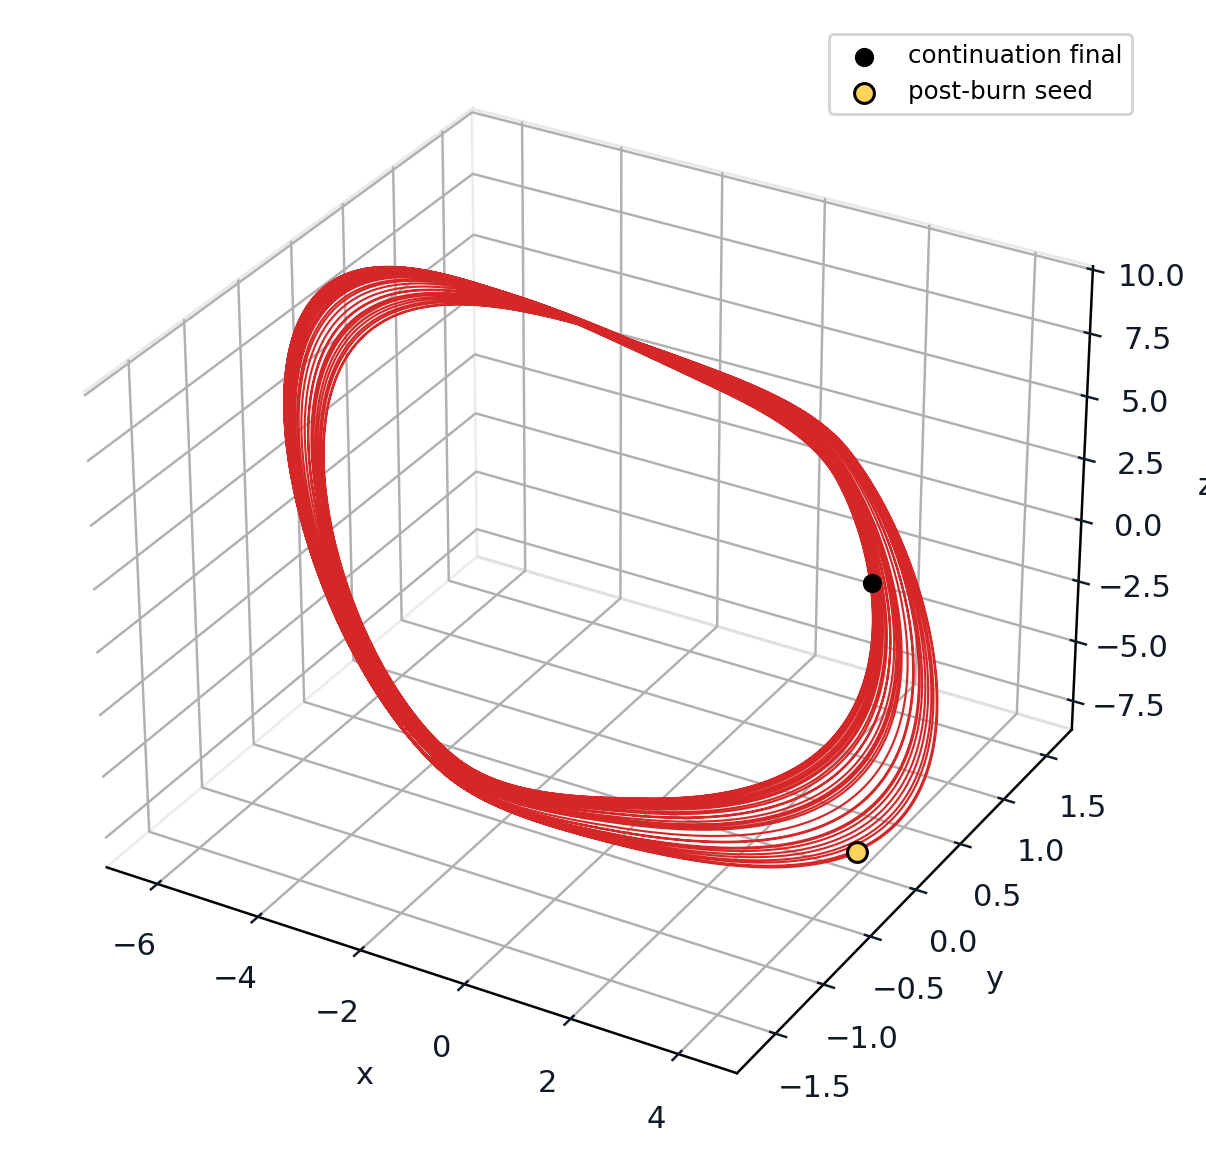
\includegraphics[width=0.82\columnwidth]{fig03_final_attractor.png}
\caption{Atractor candidato obtenido al finalizar la continuación y eliminar
el transitorio. El punto negro corresponde al estado final de continuación y
el punto amarillo a la semilla efectiva \(X_{\mathrm{target}}\).}
\label{fig:chua_int_attractor}
\end{figure}

La Fig.~\ref{fig:chua_int_hiddenness} concentra la prueba visual de ocultedad:
se comparan trayectorias iniciadas desde vecindades de los equilibrios con el
atractor candidato. En la corrida reportada no se observaron impactos hacia el
atractor objetivo desde dichas vecindades.

\begin{figure}[htbp]
\centering
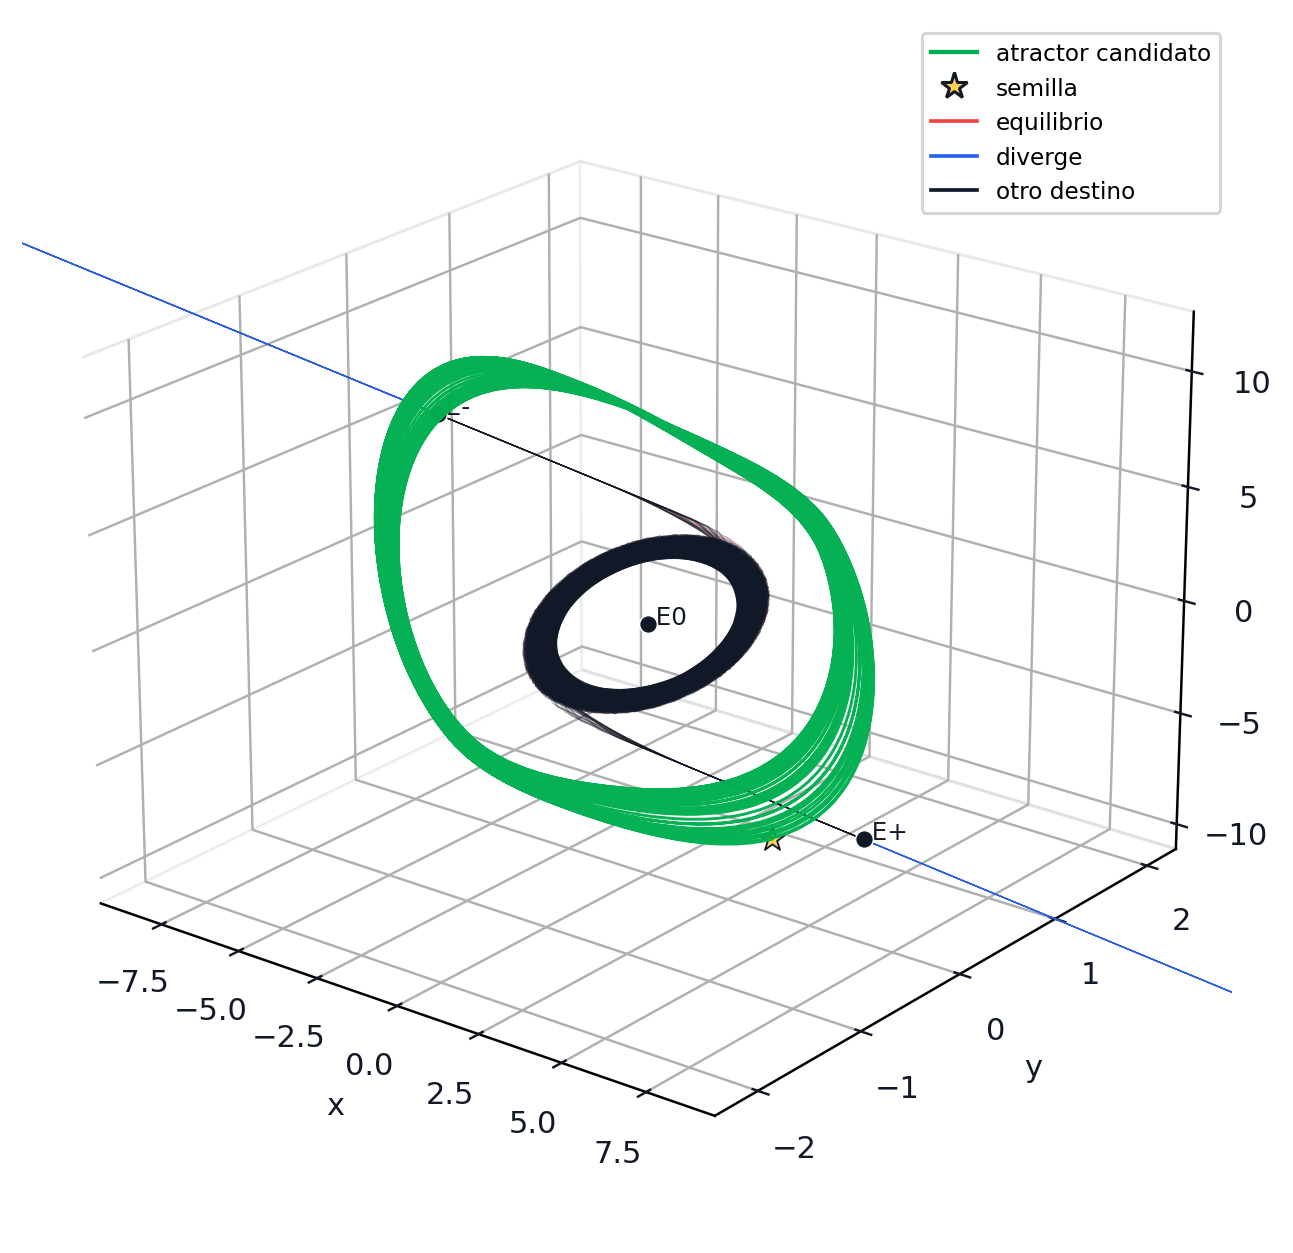
\includegraphics[width=0.82\columnwidth]{fig05b_hiddenness_overview.png}
\caption{Sondeos de ocultedad desde vecindades de los equilibrios. La ausencia
de trayectorias clasificadas como \(\mathrm{TARGET}\) apoya la clasificación
del régimen como candidato numérico a atractor oculto.}
\label{fig:chua_int_hiddenness}
\end{figure}

La Fig.~\ref{fig:chua_int_basins_xy} muestra dos cortes de cuenca en el plano
\(xy\). El primer corte fija \(z=0.\), mientras que el segundo fija
\(z=-6.53394\), valor correspondiente a la tercera coordenada de
\(X_{\mathrm{target}}\). Estos cortes permiten comparar la región cercana al
plano central con la región que contiene la semilla efectiva del atractor
candidato.

\begin{figure*}[htbp]
\centering
\subfigure[Corte \(xy\) con \(z=0.\)]{%
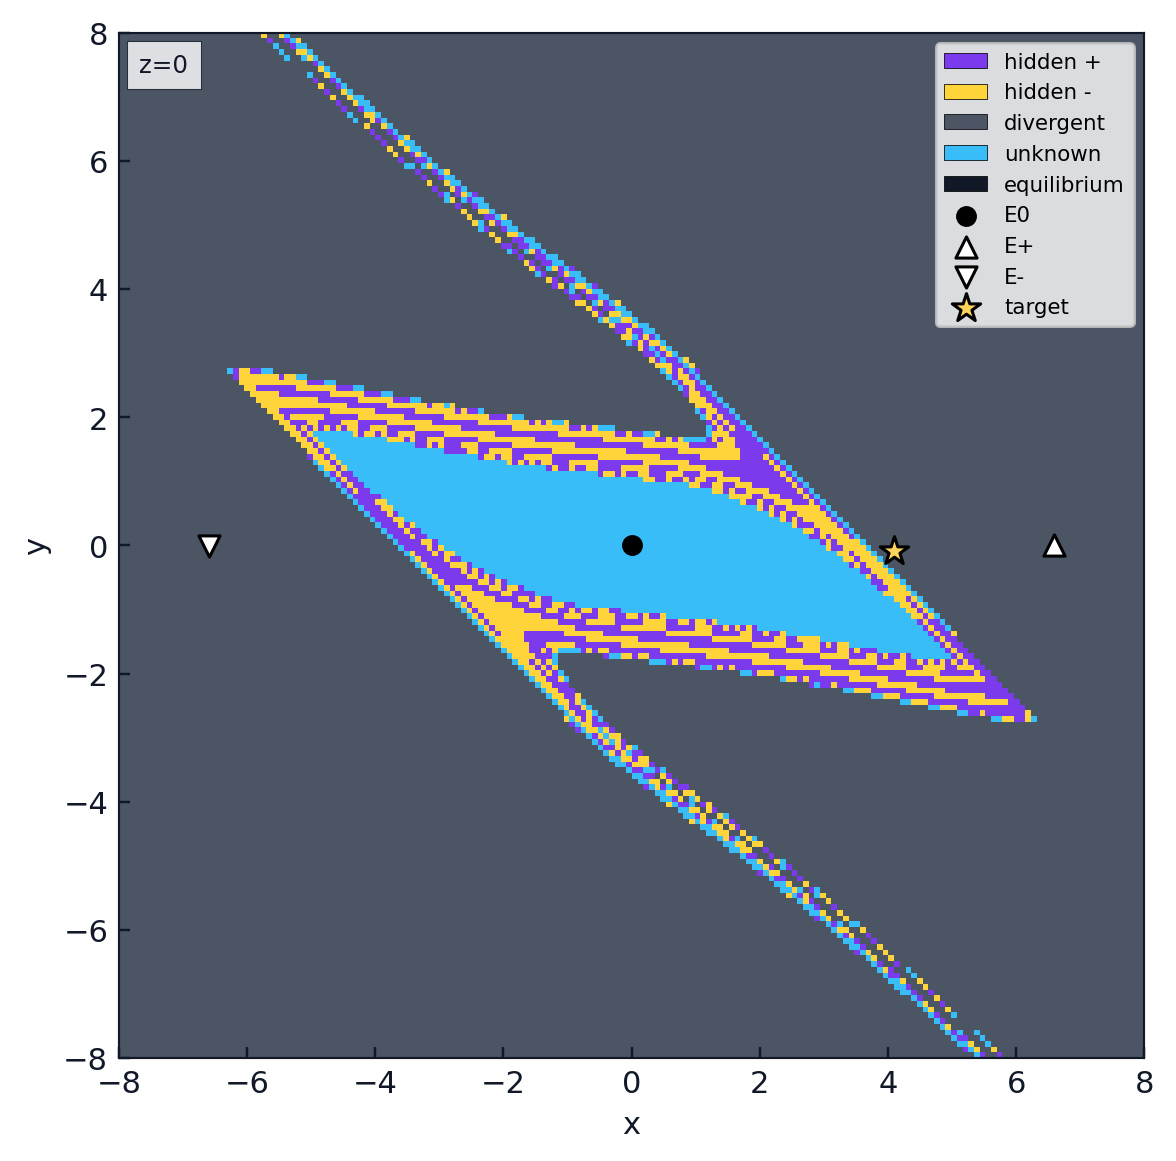
\includegraphics[width=0.8\columnwidth]{fig06a_basin_overlay_z0.png}}
\hfill
\subfigure[Corte \(xy\) con \(z=-6.53394\)]{%
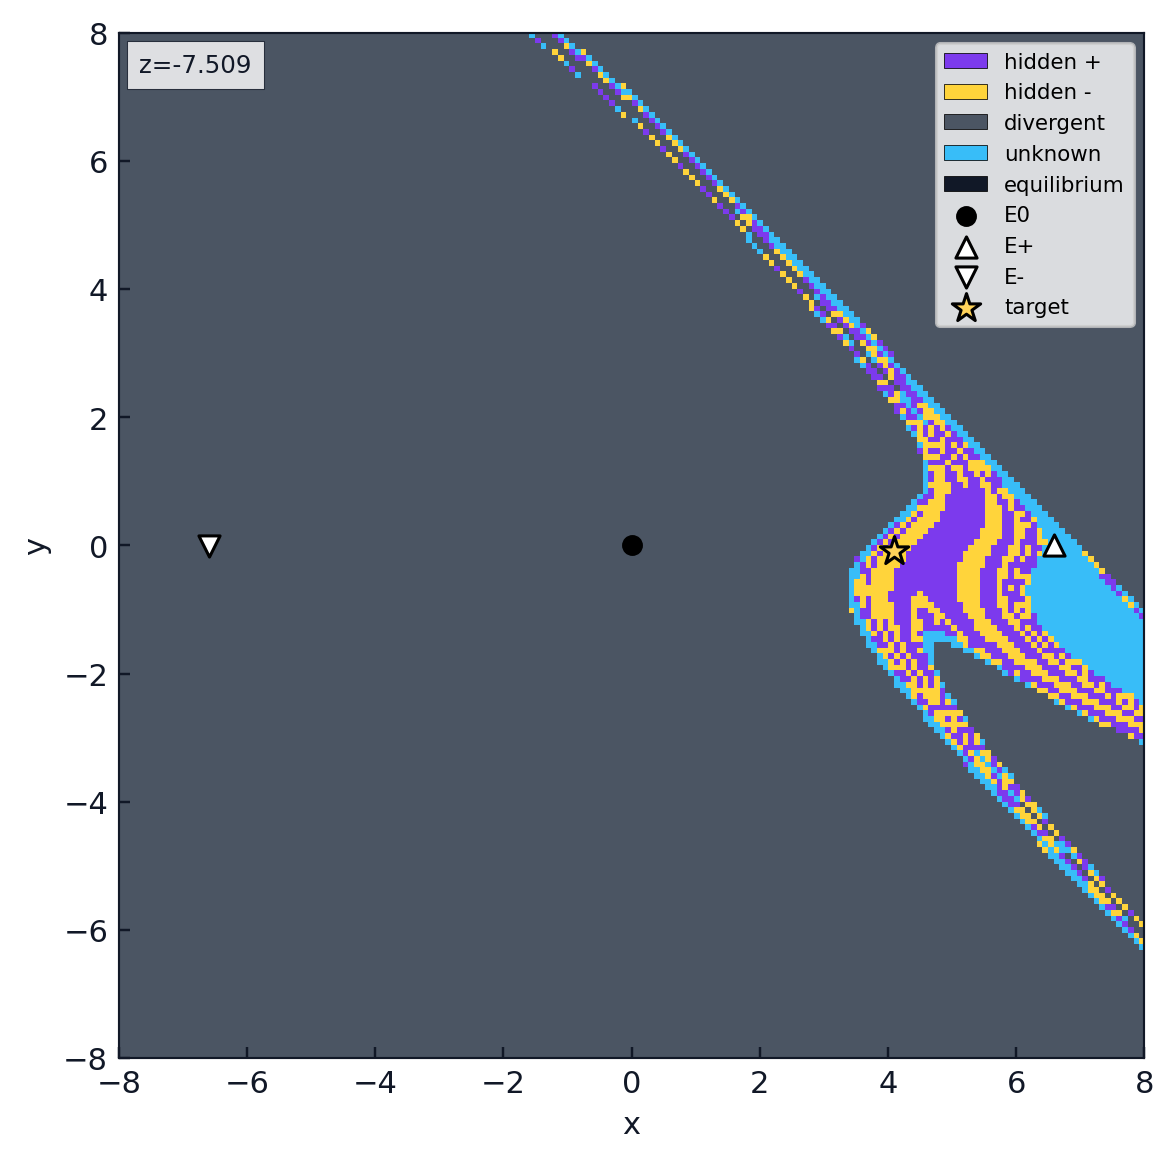
\includegraphics[width=0.8\columnwidth]{fig06b_basin_overlay_zfinal.png}}
\caption{Cuencas de atracción en dos cortes del plano \(xy\). El segundo corte
pasa por la coordenada \(z\) de la semilla efectiva
\(X_{\mathrm{target}}\), por lo que es el más directamente relacionado con el
atractor candidato.}
\label{fig:chua_int_basins_xy}
\end{figure*}

La Fig.~\ref{fig:chua_int_basins_xz_yz} muestra cortes complementarios en los
planos \(xz\) y \(yz\). Estos cortes permiten observar la extensión de la
región de atracción en direcciones transversales al plano \(xy\).

\begin{figure*}[htbp]
\centering
\subfigure[Corte \(xz\) con \(y=-0.22662\)]{%
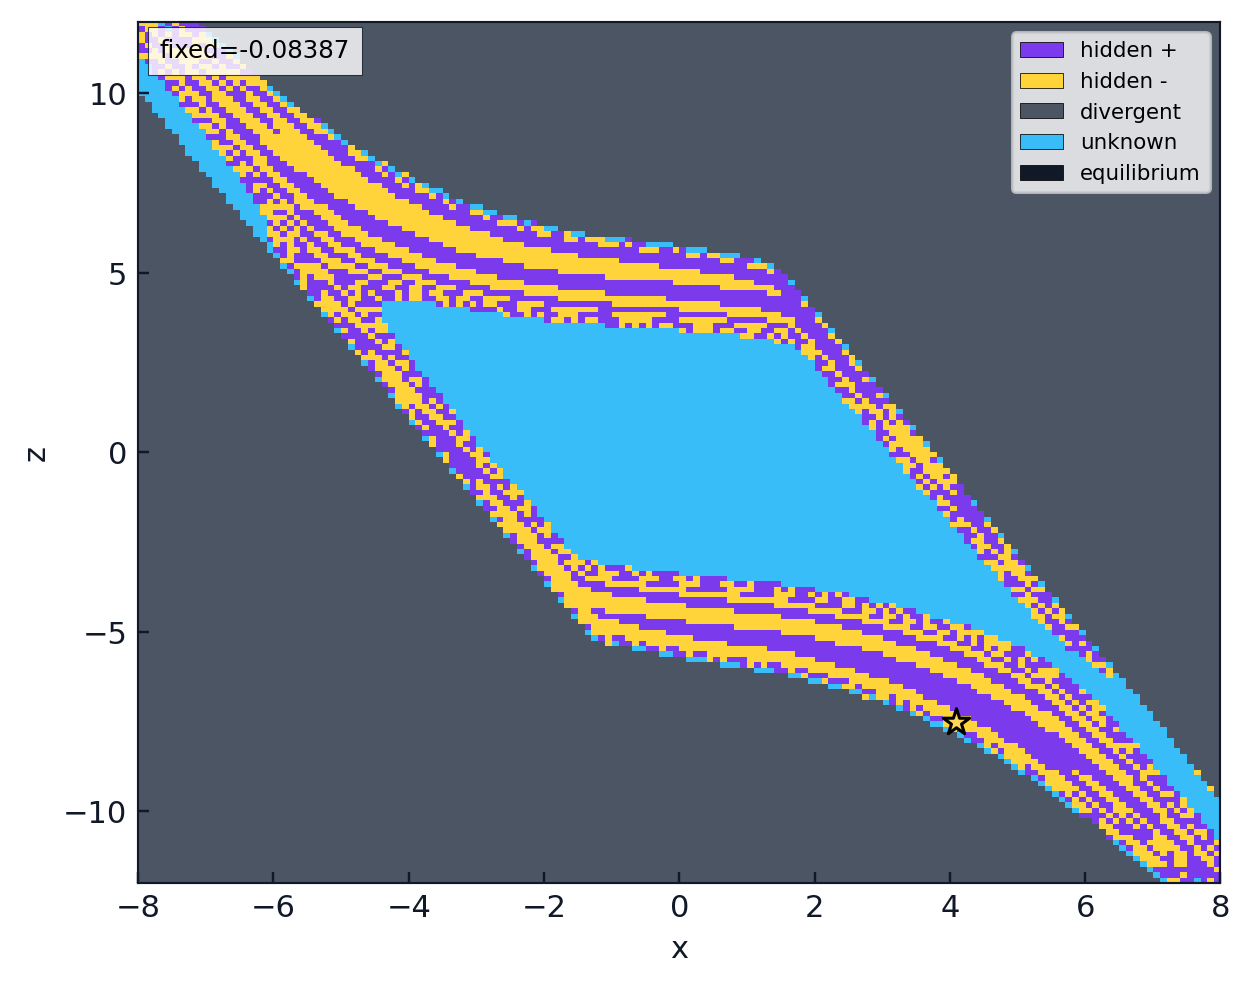
\includegraphics[width=0.8\columnwidth]{fig10b_basin_xz_final_state.png}}
\hfill
\subfigure[Corte \(yz\) con \(x=2.66011\)]{%
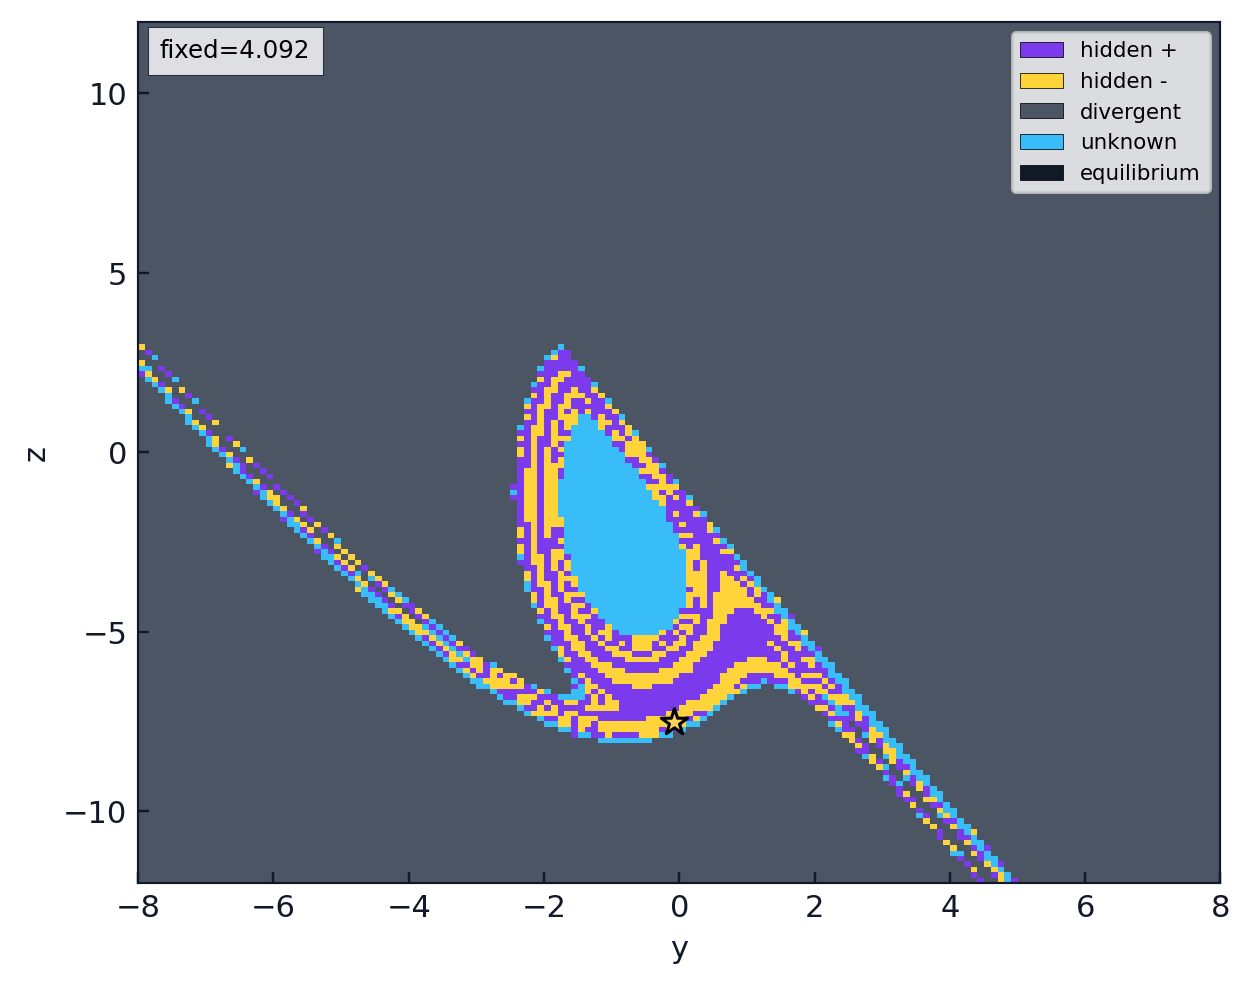
\includegraphics[width=0.8\columnwidth]{fig10c_basin_yz_final_state.png}}
\caption{Cuencas de atracción en los cortes \(xz\) y \(yz\) asociados con la
semilla efectiva \(X_{\mathrm{target}}\). Estos planos complementan los cortes
\(xy\) y muestran la estructura de cuencas alrededor de la región donde fue
localizado el atractor candidato.}
\label{fig:chua_int_basins_xz_yz}
\end{figure*}

La Fig.~\ref{fig:chua_int_fft_lyap} resume dos diagnósticos dinámicos
complementarios. La FFT de \(x(t)\), que coincide con la variable de salida
\(\sigma=r^\mathsf{T}X\), muestra una frecuencia dominante cercana a la
predicción de la función descriptiva. La convergencia de los exponentes de
Lyapunov muestra un exponente positivo, compatible con dinámica caótica.

\begin{figure}[htbp]
\centering
\subfigure[FFT de \(x(t)\)]{%
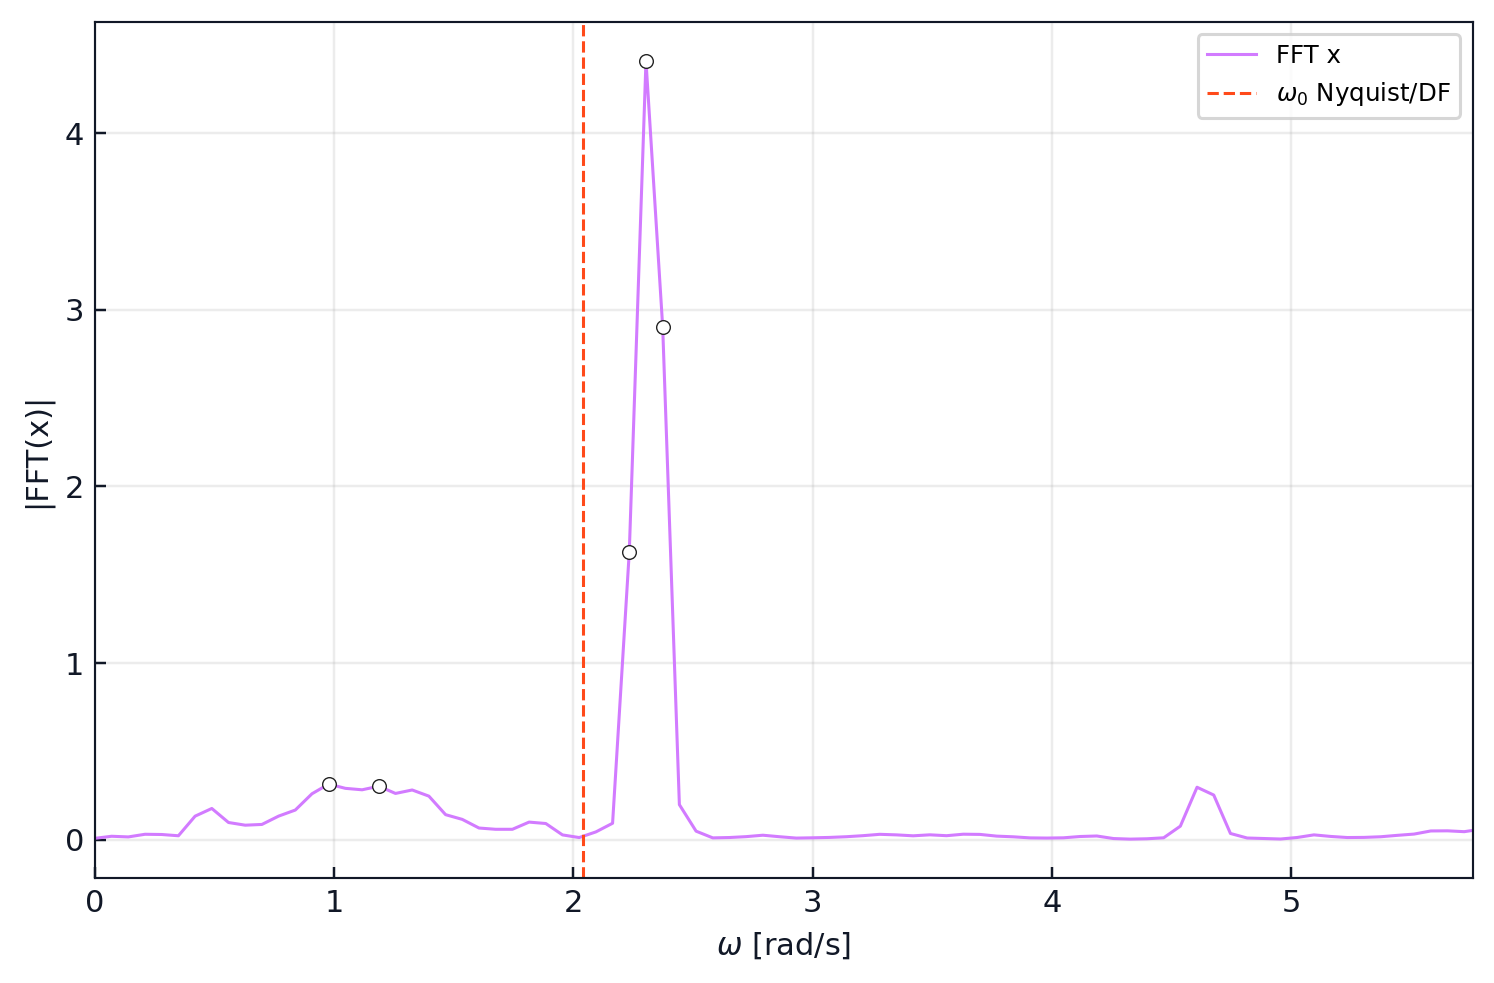
\includegraphics[width=0.82\columnwidth]{fig11a_fft_x.png}}\par\medskip
\subfigure[Convergencia de exponentes de Lyapunov]{%
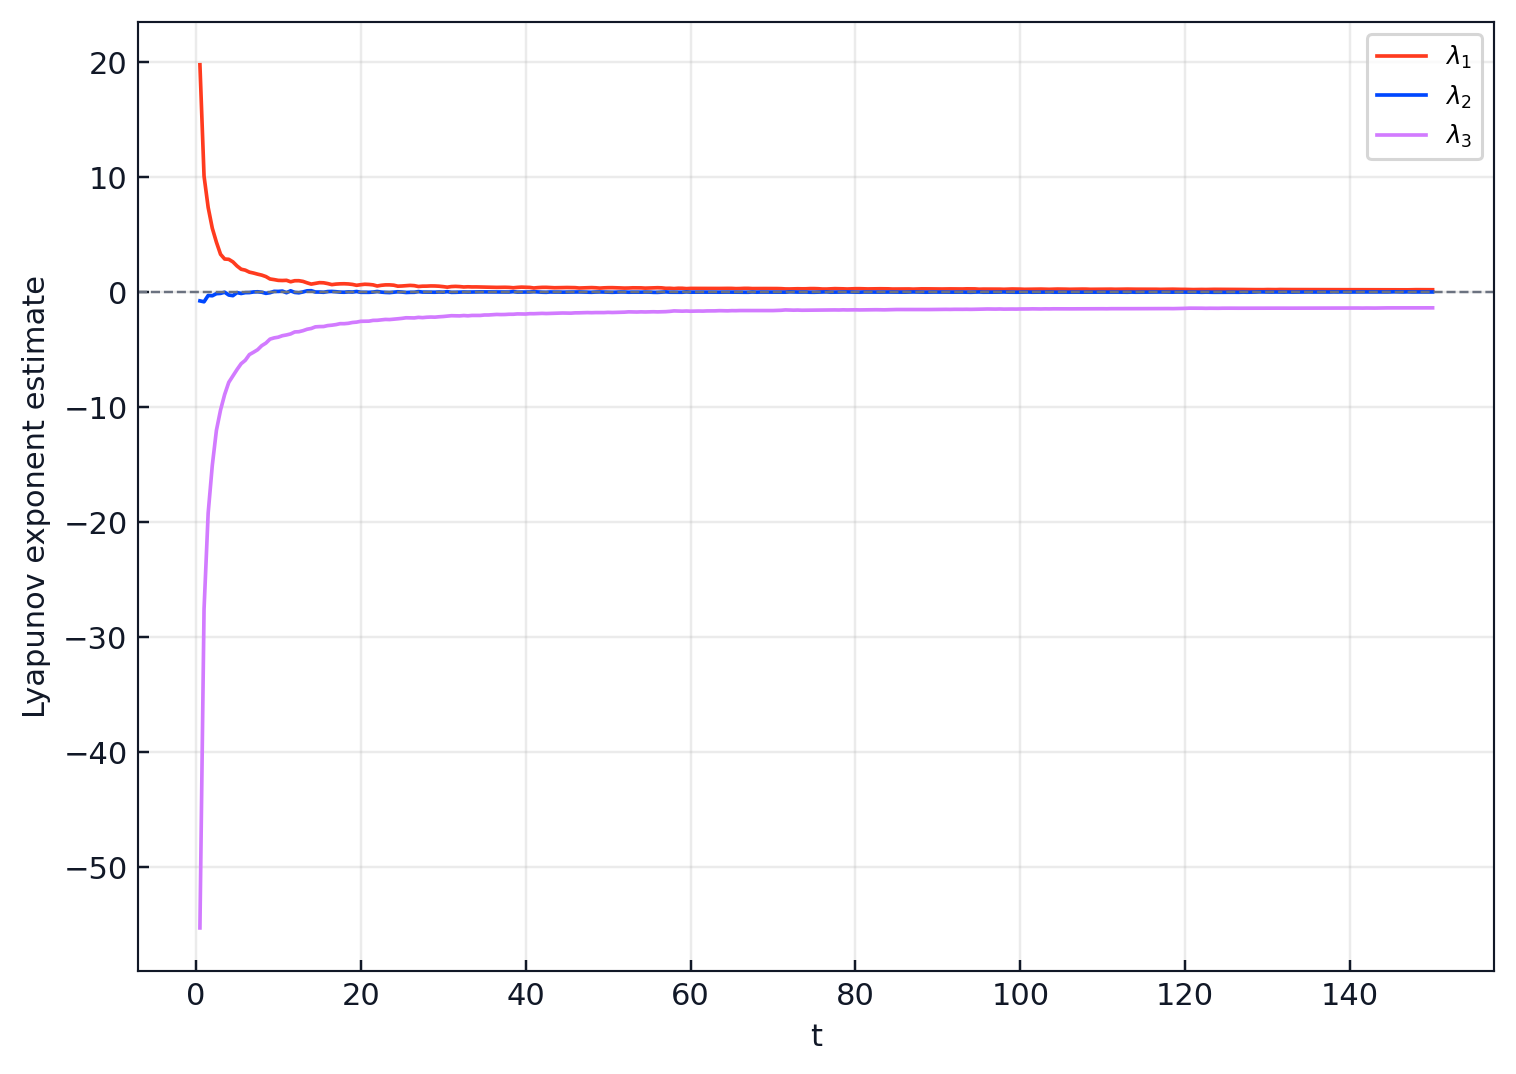
\includegraphics[width=0.82\columnwidth]{fig13_lyapunov_convergence.png}}
\caption{Diagnósticos dinámicos del régimen final. La FFT de \(x(t)\) compara
la frecuencia dominante observada con \(\omega_0\), mientras que los
exponentes de Lyapunov aportan evidencia numérica de caos.}
\label{fig:chua_int_fft_lyap}
\end{figure}

\newpage
\newpage
\subsection{Síntesis del procedimiento en orden entero}
\begin{enumerate}
\item Se construyen $P,q,r$ en \eqref{eq:Pqr}, se toma la no linealidad $\psi$ de \eqref{eq:psi_chua_def} y se calcula la función de transferencia $W(p)$ mediante \eqref{eq:Wexplicit}.
\item Se obtiene $\omega_0$ al resolver \eqref{eq:omegaeq} y, posteriormente, $k$ mediante \eqref{eq:condk}.
\item Se forma $P_0$ en \eqref{eq:P0}; luego, a partir de \eqref{eq:detP0B}--\eqref{eq:detObj} y de la identidad $W_0(p)=W_A(p)$ con \eqref{eq:W0_modificado} y \eqref{eq:WA}, se determinan $d,h,b_1,b_2$.
\item Se resuelve \eqref{eq:Phi} para obtener $a_0\ge 1$ y se verifica la condición de admisibilidad local $b_1\Phi'(a_0)<0$.
\item Se fija la condición inicial armónica en el espacio canónico mediante \eqref{eq:Y0} y se transforma a las coordenadas originales para obtener $X(0)$ con \eqref{eq:x0}.
\item Se integra el sistema derivado \eqref{eq:derived} con $\varepsilon=\varepsilon_0$ pequeño (por ejemplo, $\varepsilon_0=0.1$), usando $X(0)$ como semilla, hasta descartar transitorios y alcanzar el régimen permanente.
\item Se incrementa $\varepsilon$ sobre una malla (p.\,ej. $0.1,0.2,\dots,1.0$). En cada paso, se usa como condición inicial el último estado estacionario del paso anterior.
\item Para $\varepsilon=1$, se recupera el sistema original. El régimen alcanzado constituye un candidato a atractor oculto y debe verificarse finalmente que no sea excitado desde vecindades de los equilibrios.
\end{enumerate}

\clearpage

\section{Marco teórico del caso fraccionario}
A partir del caso de referencia, se desarrolla el ajuste teórico requerido cuando la dinámica se formula con derivada de Caputo. 

\subsection{Definiciones básicas}

Para $0<q<1$, la derivada de Caputo de una función suficientemente regular $x:[0,T]\to\R^n$ se define por
\begin{equation}
\CaputoD{q}x(t)=\frac{1}{\Gamma(1-q)}\int_0^t (t-\tau)^{-q}\,\dot x(\tau)\,d\tau.
\label{eq:caputo_def}
\end{equation}

\noindent El problema autónomo de orden fraccionario
\begin{equation}
\CaputoD{q}x(t)=f(x(t)),\qquad x(0)=x_0,
\label{eq:fode_caputo}
\end{equation}
se reescribe como ecuación integral de Volterra
\begin{equation}
 x(t)=x_0+\frac{1}{\Gamma(q)}\int_0^t (t-\tau)^{q-1}f(x(\tau))\,d\tau.
\label{eq:volterra_caputo}
\end{equation}

\noindent La ecuación \eqref{eq:volterra_caputo} muestra la principal diferencia que tiene el caso fraccionario con el caso entero. En \eqref{eq:fode_caputo}, el campo vectorial es la aplicación $f:\R^n\to\R^n$ y el término $f(x(t))$ representa su evaluación en el estado actual $x(t)$. La memoria no reside en ese campo vectorial local, sino en el operador de Caputo ---o, equivalentemente, en el núcleo integral de \eqref{eq:volterra_caputo}---, por lo que la evolución en tiempo $t$ depende de toda la historia de la trayectoria en el intervalo $[0,t]$.

\subsection{Justificación de la linealización usando el jacobiano}

Sea el sistema fraccionario autónomo
\[
{}^{C}D_t^q x(t)=F(x(t)),\qquad 0<q<1,
\]
y sea \(x^\ast\) un equilibrio,
\[
F(x^\ast)=0.
\]
Se supone que \(F\in C^1(U,\mathbb R^n)\)\footnote{Significa que \(F\) es continuamente diferenciable en \(U\), todas sus derivadas parciales de primer orden existen y son continuas.} en una vecindad abierta \(U\) de \(x^\ast\). Al introducir la perturbación
\[
\xi(t)=x(t)-x^\ast,
\]
se obtiene
\[
{}^{C}D_t^q\big(x^\ast+\xi(t)\big)=F(x^\ast+\xi(t)).
\]
Como la derivada de Caputo de una constante es cero,
\[
{}^{C}D_t^q \xi(t)=F(x^\ast+\xi(t)).
\]

Por diferenciabilidad de Fréchet\footnote{La derivada de Fréchet es la generalización de la derivada del cálculo clásico y es el operador lineal que proporciona la mejor aproximación local de \(F\) cerca de un punto \cite{Deimling1985,Khalil2002}
\[
F(x^\ast+\xi)=F(x^\ast)+DF(x^\ast)\xi+o(\|\xi\|).
\]
} de \(F\) en \(x^\ast\), existe un operador lineal
\[
DF(x^\ast):\mathbb R^n\to\mathbb R^n
\]
tal que
\[
F(x^\ast+\xi)
=
F(x^\ast)+DF(x^\ast)\xi+R(\xi),
\qquad
\lim_{\xi\to0}\frac{\|R(\xi)\|}{\|\xi\|}=0. 
\]
En coordenadas finitas, el operador \(DF(x^\ast)\) queda representado por la matriz jacobiana.
\[
J(x^\ast)=
\left[
\frac{\partial F_i}{\partial x_j}(x^\ast)
\right]_{i,j=1}^{n}.
\]
Como \(F(x^\ast)=0\), resulta
\[
{}^{C}D_t^q \xi(t)
=
J(x^\ast)\xi(t)+R(\xi(t)).
\]
Al despreciar el residuo de orden superior \(R(\xi)=o(\|\xi\|)\), se obtiene el sistema linealizado local
\begin{equation}
\label{eq:lin_eq}
{}^{C}D_t^q \xi(t)=J(x^\ast)\xi(t).
\end{equation}

La linealización \eqref{eq:lin_eq} actúa sobre la geometría local del campo \(F\), mientras que la no localidad permanece en el operador temporal de Caputo y no elimina la memoria fraccionaria. Por lo tanto, el jacobiano sigue siendo consistente para la aproximación lineal local. La estabilidad del sistema linealizado se decide con criterios fraccionarios tipo Matignon y con estabilidad de Mittag--Leffler \cite{Matignon1996,LiMa2013,LiChenPodlubny2009}.

\subsection{Memoria fraccionaria y continuación por ventana de historia}

La formulación integral \eqref{eq:volterra_caputo} muestra que, en una ecuación de Caputo, la evolución posterior no depende sólo del estado actual \(x(t_j)\), sino también de la historia previa de la trayectoria. Esta dependencia proviene del núcleo \((t-\tau)^{q-1}\), que pondera los valores pasados de \(f(x(\tau))\). Por ello, a diferencia de una EDO ordinaria, no se puede asumir en general que la solución tenga una propiedad de semigrupo en el sentido clásico: reiniciar la integración desde \(x(t_j)\) no reproduce necesariamente el mismo problema histórico \cite{LiMa2013}.

En una continuación numérica de sistemas de Caputo, esta observación implica que el paso de un nivel \(\varepsilon_j\) a otro \(\varepsilon_{j+1}\) no debe hacerse usando únicamente el punto terminal \(x_j(t_{\rm end})\). Para una familia homotópica
\[
{}^CD_t^q x=F(x;\varepsilon),
\qquad \varepsilon\in[0,1],
\]
el reinicio desde un solo punto elimina parte de la memoria acumulada y cambia el protocolo causal del problema. En métodos con memoria corta, la truncación de historia es una aproximación controlada del operador no una eliminación arbitraria de la memoria previa \cite{Deng2007,MendesSalgadoAguirre2019,HaiYuXuRen2022}.

Esto es relevante cuando existen cuencas delgadas, coexistencia de atractores o sensibilidad fuerte a la historia. En tales casos, un reinicio sólo desde \(x_j(t_{\rm end})\) puede llevar la trayectoria a otra cuenca de atracción o producir una semilla numéricamente plausible pero no reproducible bajo el mismo operador de memoria\cite{LeonovKuznetsov2013,KuznetsovEtAl2017,Danca2017,GuanXie2025}.

En este trabajo se usa una aproximación de memoria corta. Si \(L_m\) denota la longitud efectiva de memoria, se aproxima esquemáticamente
\[
{}^CD_{t,L_m}^{q}x(t)
\approx
\frac{1}{\Gamma(1-q)}
\int_{t-L_m}^{t}(t-\tau)^{-q}\dot x(\tau)\,d\tau .
\]
Por tanto, entre pasos de continuación se transporta el segmento terminal
\[
\mathcal H_j=
\left\{x_j(t):t\in[t_{\rm end}-L_m,t_{\rm end}]\right\}.
\]
Si el integrador reinicia el siguiente paso con un nuevo origen temporal \(t_{\rm start}\), la condición histórica se reindexa como
\[
x_{j+1}(t_{\rm start}+\theta)
=
x_j(t_{\rm end}+\theta),
\qquad -L_m\leq\theta\leq 0.
\]
Esta igualdad preserva la ventana de memoria reciente usada por el operador truncado. Así, en la continuación numérica se transporta progresivamente  una trayectoria junto con su memoria efectiva.

\subsection{Balance armónico y puente Weyl--Caputo}

En el caso fraccionario, el balance armónico no se interpreta directamente sobre el sistema autónomo de Caputo, porque éste no admite en general soluciones periódicas exactas no constantes con límite inferior fijo \cite{TavazoeiHaeri2009,AreaLosadaNieto2014}. Por ello, la función descriptiva se formula sobre un problema auxiliar en el marco de Weyl/Liouville--Weyl \cite{Vigue2019}, donde las exponenciales armónicas sí son autofunciones del operador. Al escribir \(s=i\omega\), se cumple 
\[
{}^{LW}D_t^q e^{i\omega t}=s^q e^{i\omega t}.
\]
Ésta es la razón por la que el problema de Weyl sirve para construir el predictor frecuencial, mientras que el problema de Caputo se reserva para la integración y la validación final.

El paso desde ese problema auxiliar al sistema causal de Caputo se justifica mediante el puente Weyl--Caputo. En la identidad
\[
D_{-\infty}^{q}x(t)=\,{}^{C}D_{t_0}^{q}x(t)+\mathcal E_{x_0}(t),
\]
el término de la izquierda representa la derivada con historia infinita propia del marco de Weyl; el primer sumando del lado derecho es la derivada causal de Caputo iniciada en \(t_0\); y \(\mathcal E_{x_0}(t)\) recoge la contribución del pasado remoto anterior a \(t_0\). Siguiendo la descomposición expuesta por \cite{Haacker2026}, dicho término puede escribirse como
\[
\mathcal E_{x_0}(t)
=
\frac{1}{\Gamma(1-q)}
\int_{-\infty}^{t_0}(t-\tau)^{-q}x_0'(\tau)\,d\tau.
\]
En ese sentido, una definición natural de la función de error es
\[
e_{WC}(t):=D_{-\infty}^{q}x(t)-{}^{C}D_{t_0}^{q}x(t)=\mathcal E_{x_0}(t).
\]
Además, este término satisface la cota algebraica
\[
\|\mathcal E_{x_0}(t)\|\le C\,(t-t_0+\eta)^{-q},
\qquad t\ge t_0,
\]
para una constante \(C>0\) dependiente de la historia inicial \cite{Haacker2026}. En consecuencia, el problema de Caputo puede leerse como el problema periódico de Weyl perturbado por un término de memoria residual que se atenúa con el tiempo. Ésa es la justificación para usar la órbita armónica auxiliar de Weyl como semilla asintóticamente consistente del problema de Caputo, aunque esta no represente precisamente un ciclo límite exacto.



\subsection{Justificación de la función descriptiva y del balance armónico}

Considérese un sistema fraccionario de Caputo en forma tipo Lur'e,
\begin{equation}
\label{eq:lure_frac_general}
{}^{C}D_t^q x
=
Px+b\,\phi(\sigma),
\qquad
\sigma=r^\top x,
\qquad
0<q<1.
\end{equation}
En el caso fraccionario se conserva la separación entre un bloque lineal
dinámico y un bloque no lineal escalar. Lo que cambia respecto al caso
entero es la relación de transferencia del bloque lineal. Para \(0<q<1\),
la transformada de Laplace de la derivada de Caputo es
\[
\mathcal L\left\{{}^{C}D_t^q x(t)\right\}(s)
=
s^qX(s)-s^{q-1}x(0).
\]
Al definir una función de transferencia se consideran condiciones iniciales
nulas, por lo que
\[
\mathcal L\left\{{}^{C}D_t^q x(t)\right\}(s)
=
s^qX(s).
\]
Por tanto, el operador algebraico asociado al bloque lineal fraccionario es
\(s^q I-P\) \cite{Podlubny1999,Monje2010}.

Para el bloque lineal
\[
{}^{C}D_t^q x = P x + b\,u,
\qquad
\sigma=r^\top x,
\]
la función de transferencia entrada--salida queda
\begin{equation}
\label{eq:Wq_frac_teorico}
W_q(s)
=
r^\top(s^q I-P)^{-1}b.
\end{equation}
Sobre el eje imaginario se evalúa \(s=i\omega\). En la rama principal,
\begin{equation}
\label{eq:sq_freq_frac}
s^q
=
\omega^q
\left(
\cos\frac{q\pi}{2}
+
i\sin\frac{q\pi}{2}
\right).
\end{equation}
Así,
\begin{equation}
\label{eq:Wq_frac_imag_teorico}
W_q(i\omega)
=
r^\top\bigl(s^q I-P\bigr)^{-1}b.
\end{equation}

La función descriptiva se aplica al bloque no lineal. Si la entrada al
bloque no lineal es
\[
\sigma(t)=a\sin(\omega t),
\]
entonces, con \(\theta=\omega t\),
\[
y(\theta)=\phi(a\sin\theta).
\]
En general, \(y(\theta)\) no es sinusoidal. La función descriptiva sustituye
esta salida por su componente fundamental,
\[
y_1(\theta)
=
\alpha_1(a)\sin\theta+\beta_1(a)\cos\theta,
\]
donde
\[
\alpha_1(a)
=
\frac{1}{\pi}
\int_{-\pi}^{\pi}
\phi(a\sin\theta)\sin\theta\,d\theta,
\]
\[
\beta_1(a)
=
\frac{1}{\pi}
\int_{-\pi}^{\pi}
\phi(a\sin\theta)\cos\theta\,d\theta.
\]
Con la convención compleja adoptada,
\begin{equation}
\label{eq:DF_general}
N_\phi(a)
=
\frac{\alpha_1(a)-i\beta_1(a)}{a}.
\end{equation}
Si \(\phi\) es estática, impar y monovaluada, entonces
\[
\beta_1(a)=0,
\]
y
\begin{equation}
\label{eq:DF_impar}
\begin{aligned}
N_\phi(a)
&=
\frac{1}{\pi a}
\int_{-\pi}^{\pi}
\phi(a\sin\theta)\sin\theta\,d\theta\\
&=
\frac{2}{\pi a}
\int_{0}^{\pi}
\phi(a\sin\theta)\sin\theta\,d\theta.
\end{aligned}
\end{equation}

La integral \eqref{eq:DF_impar} no contiene operadores fraccionarios. Por
tanto, si la no linealidad es estática, su ganancia equivalente depende de
la amplitud \(a\), pero no depende directamente del orden \(q\). La
fraccionalidad aparece en la propagación del primer armónico a través del
bloque lineal, es decir, en \(W_q(i\omega)\).

El balance armónico de primer orden se plantea entonces como
\begin{equation}
\label{eq:balance_frac_Wq}
1+W_q(i\omega)N_\phi(a)=0.
\end{equation}
Cuando \(N_\phi(a)\) es real, la condición anterior implica
\[
\Im\{W_q(i\omega_0)\}=0,
\]
y
\begin{equation}
\label{eq:amp_balance_frac}
N_\phi(a_0)
=
-\frac{1}{\Re\{W_q(i\omega_0)\}}.
\end{equation}
Así, \(\omega_0\) se obtiene de la condición de fase del bloque lineal
fraccionario, mientras que \(a_0\) se obtiene resolviendo la ecuación de
amplitud \eqref{eq:amp_balance_frac}.

En este trabajo, la función descriptiva clásica se interpreta como una
proyección de primer armónico. No proporciona una representación exacta de
la no linealidad, sino una ganancia equivalente válida para el problema
auxiliar armónico. Por ello, el par \((a_0,\omega_0)\) no prueba la
existencia de un ciclo límite exacto del sistema de Caputo; sólo proporciona
una frecuencia dominante y una amplitud candidata para construir semillas
iniciales. El balance armónico se usa aquí como
aproximación asintótica y como generador de semillas, no como prueba de
periodicidad exacta \cite{TavazoeiHaeri2009,KaslikSivasundaram2012,Vigue2019,Haacker2026}.


\subsection{Alcance y límite en orden fraccionario}

Haacker et al. en \cite{Haacker2026} muestran que una extensión fraccionaria de ese enfoque sólo permite capturar soluciones exponencialmente crecientes; no describe de forma adecuada las soluciones estables con decaimiento algebraico. Por tanto, la función descriptiva y el balance armónico sí sirven para el \emph{predictor}, pero la validación estable del régimen final recae en la integración y en la verificación numérica posterior haciendo una exploración de las trayectorias alrededor de los puntos de equilibrio y de la cuenca de atracción del sistema.

\section{Ejemplo de estudio I: Chua fraccionario no suave}
\label{sec:chua_nonsmooth_frac}

\subsection{Sistema de partida}

Se considera el sistema de Chua fraccionario con no linealidad de saturación, en orden conmensurado $q\in(0,1]$ y con derivada de Caputo:
\begin{equation}
\label{eq:chua_ns_system}
\begin{aligned}
{}^{C}D_t^q x_1 &= \alpha\bigl(x_2-x_1-m_1x_1-\psi(x_1)\bigr),\\
{}^{C}D_t^q x_2 &= x_1-x_2+x_3,\\
{}^{C}D_t^q x_3 &= -\beta x_2-\gamma x_3,
\end{aligned}
\end{equation}
donde
\begin{equation}
\label{eq:psi_ns_def}
\psi(\sigma)=(m_0-m_1)\operatorname{sat}(\sigma),
\end{equation}
con la función de saturación \(\operatorname{sat}\) definida previamente en \eqref{eq:sat_chua}.
Este modelo se adopta como primer caso de estudio porque la no linealidad queda concentrada en una función escalar impar y estática, lo que permite aplicar de manera directa la separación tipo Lur'e. La formulación coincide con el caso no suave reportado por Danca para la búsqueda de atractores ocultos en sistemas fraccionarios \cite{Danca2017}. 

\subsection{Equilibrios y estabilidad local}

La derivada existe fuera de las superficies de conmutación
$x_1=\pm 1$ y queda dada por
\begin{equation}
\psi'(x_1)=
\begin{cases}
0, & |x_1|>1,\\[1mm]
m_0-m_1, & |x_1|<1.
\end{cases}
\end{equation}

En equilibrio se cumple
\begin{equation}
\label{eq:ns_equilibrium_conditions}
\begin{aligned}
0&=\alpha(x_2-x_1-m_1x_1-\psi(x_1)),\\
0&=x_1-x_2+x_3,\\
0&=-\beta x_2-\gamma x_3.
\end{aligned}
\end{equation}
De la segunda ecuación,
\[
x_3=x_2-x_1.
\]
Sustituyendo en la tercera ecuación,
\[
0=-\beta x_2-\gamma(x_2-x_1)
=-(\beta+\gamma)x_2+\gamma x_1.
\]
Como \(\beta+\gamma\neq 0\), se obtiene
\begin{equation}
\label{eq:yz_equilibrio_ns}
x_2^*=\frac{\gamma}{\beta+\gamma}x_1^*,
\qquad
x_3^*
=
x_2^*-x_1^*
=
-\frac{\beta}{\beta+\gamma}x_1^*.
\end{equation}

Definiendo
\begin{equation}
\label{eq:rho_A_delta_ns}
\rho\coloneqq \frac{\gamma}{\beta+\gamma},
\qquad
A_{\rm eq}\coloneqq 1+m_1-\rho,
\qquad
\Delta\coloneqq m_0-m_1,
\end{equation}
la primera ecuación de equilibrio queda
\[
0=
\alpha\left[
\rho x_1^*-(1+m_1)x_1^*-\psi(x_1^*)
\right].
\]
Como \(\alpha\neq 0\), esto equivale a
\[
\rho x_1^*-(1+m_1)x_1^*-\psi(x_1^*)=0.
\]
Multiplicando por \(-1\), se obtiene la ecuación escalar
\begin{equation}
\label{eq:scalar_equilibrium_ns}
A_{\rm eq} x_1^*+\psi(x_1^*)=0,
\end{equation}
es decir,
\begin{equation}
\left(1+m_1-\frac{\gamma}{\beta+\gamma}\right)x_1^*
+
\psi(x_1^*)=0.
\end{equation}

El análisis debe hacerse por regiones.

Para \(|x_1^*|<1\), se tiene \(\psi(x_1^*)=\Delta x_1^*\). Entonces
\[
A_{\rm eq} x_1^*+\Delta x_1^*
=
(A_{\rm eq}+\Delta)x_1^*
=
\left(
1+m_0-\frac{\gamma}{\beta+\gamma}
\right)x_1^*
=0.
\]
Si
\[
1+m_0-\frac{\gamma}{\beta+\gamma}\neq 0,
\]
el único equilibrio interno es
\begin{equation}
\label{eq:origin_equilibrium_ns}
x_1^*=0.
\end{equation}
Por tanto,
\begin{equation}
\label{eq:equilibria_ns_origin}
X_0^*=(0,0,0).
\end{equation}

Para \(x_1^*>1\), se tiene \(\psi(x_1^*)=\Delta\). Entonces
\[
A_{\rm eq} x_1^*+\Delta=0,
\]
de donde
\begin{equation}
\label{eq:x_plus_ns}
x_{1,+}^*=-\frac{\Delta}{A_{\rm eq}}
=
-\frac{m_0-m_1}{
1+m_1-\dfrac{\gamma}{\beta+\gamma}
}.
\end{equation}
Para \(x_1^*<-1\), se tiene \(\psi(x_1^*)=-\Delta\). Entonces
\[
A_{\rm eq} x_1^*-\Delta=0,
\]
de donde
\begin{equation}
\label{eq:x_minus_ns}
x_{1,-}^*=\frac{\Delta}{A_{\rm eq}}
=
\frac{m_0-m_1}{
1+m_1-\dfrac{\gamma}{\beta+\gamma}
}.
\end{equation}
Estos equilibrios externos son admisibles sólo si
\[
x_{1,+}^*>1,
\qquad
x_{1,-}^*<-1.
\]

En forma compacta, los equilibrios se escriben como
\begin{equation}
\label{eq:X_equilibrium_map_ns}
X^*(x_1^*)
=
\begin{bmatrix}
x_1^*\\[1mm]
\dfrac{\gamma}{\beta+\gamma}x_1^*\\[3mm]
-\dfrac{\beta}{\beta+\gamma}x_1^*
\end{bmatrix}.
\end{equation}
Por tanto,
\begin{equation}
X_0^*=X^*(0),
\qquad
X_+^*=X^*(x_{1,+}^*),
\qquad
X_-^*=X^*(x_{1,-}^*).
\end{equation}

Para los parámetros
\begin{equation}
  \label{eq:danca_params_ns}
  \begin{aligned}
\alpha&=8.4562, & \beta&=12.0732, & \gamma&=0.0052,\\
m_0&=-0.1768, & m_1&=-1.1468.
\end{aligned}
\end{equation}

se obtiene
\[
\rho=
\frac{\gamma}{\beta+\gamma}
\approx
4.30521\times 10^{-4},
\]
\[
\begin{aligned}
A_{\rm eq}&=1+m_1-\rho \approx -0.14723,\\
\Delta&=m_0-m_1=0.97.
\end{aligned}
\]
Por tanto,
\[
\begin{aligned}
x_{1,+}^*&=-\frac{\Delta}{A_{\rm eq}}\approx 6.58831,\\
x_{1,-}^*&=\frac{\Delta}{A_{\rm eq}}\approx -6.58831.
\end{aligned}
\]
Así,
\begin{equation}
\label{eq:equilibria_ns_values}
X_0^*=(0,0,0),
\end{equation}
\begin{equation}
\label{eq:equilibria_ns_values_pm}
X_\pm^*
\approx
\begin{bmatrix}
\pm 6.58831\\
\pm 2.83640\times 10^{-3}\\
\mp 6.58547
\end{bmatrix}.
\end{equation}

La matriz jacobiana general del campo vectorial, en los puntos donde
\(\psi\) es diferenciable, es
\begin{equation}
J(X)
=
\begin{bmatrix}
-\alpha(1+m_1+\psi'(x_1)) & \alpha & 0\\
1 & -1 & 1\\
0 & -\beta & -\gamma
\end{bmatrix}.
\end{equation}
En la región interna \(|x_1|<1\), como \(\psi'(x_1)=m_0-m_1\), se obtiene
\begin{equation}
\label{eq:J_ns_inner}
J_{\rm in}
=
\begin{bmatrix}
-\alpha(1+m_0)&\alpha&0\\
1&-1&1\\
0&-\beta&-\gamma
\end{bmatrix}.
\end{equation}
En la región externa \(|x_1|>1\), como \(\psi'(x_1)=0\), se obtiene
\begin{equation}
\label{eq:J_ns_outer}
J_{\rm out}
=
\begin{bmatrix}
-\alpha(1+m_1)&\alpha&0\\
1&-1&1\\
0&-\beta&-\gamma
\end{bmatrix}.
\end{equation}

Para verificar algebraicamente los autovalores, sea
\[
\mu=
\begin{cases}
m_0, & \text{región interna},\\
m_1, & \text{región externa},
\end{cases}
\]
y defínase
\begin{equation}
J_\mu
=
\begin{bmatrix}
-\alpha(1+\mu)&\alpha&0\\
1&-1&1\\
0&-\beta&-\gamma
\end{bmatrix}.
\end{equation}
Entonces
\[
\lambda I-J_\mu
=
\begin{bmatrix}
\lambda+\alpha(1+\mu)&-\alpha&0\\
-1&\lambda+1&-1\\
0&\beta&\lambda+\gamma
\end{bmatrix}.
\]
Calculando el determinante por la primera fila,
\begin{align}
\chi_\mu(\lambda)
&=
\det(\lambda I-J_\mu)
\\
&=
\left[\lambda+\alpha(1+\mu)\right]
\det
\begin{bmatrix}
\lambda+1&-1\\
\beta&\lambda+\gamma
\end{bmatrix}
\nonumber\\
&\quad
+\alpha
\det
\begin{bmatrix}
-1&-1\\
0&\lambda+\gamma
\end{bmatrix}.
\end{align}
Los menores son
\[
\begin{aligned}
\det
\begin{bmatrix}
\lambda+1&-1\\
\beta&\lambda+\gamma
\end{bmatrix}
&=(\lambda+1)(\lambda+\gamma)+\beta\\
&=\lambda^2+(1+\gamma)\lambda+(\beta+\gamma).
\end{aligned}
\]
y
\[
\det
\begin{bmatrix}
-1&-1\\
0&\lambda+\gamma
\end{bmatrix}
=
-(\lambda+\gamma).
\]
Por tanto,
\begin{equation}
\label{eq:char_poly_mu_ns}
\begin{aligned}
\chi_\mu(\lambda)
&=
\left[\lambda+\alpha(1+\mu)\right]
\left[
\lambda^2+(1+\gamma)\lambda+(\beta+\gamma)
\right]\\
&\quad-\alpha(\lambda+\gamma).
\end{aligned}
\end{equation}
Al expandir,
\begin{align}
\chi_\mu(\lambda)
&=
\lambda^3
+
\left[
\alpha(1+\mu)+1+\gamma
\right]\lambda^2
\nonumber\\
&\quad+
\left[
\beta+\gamma
+
\alpha(1+\mu)(1+\gamma)
-\alpha
\right]\lambda
\nonumber\\
&\quad+
\alpha(1+\mu)(\beta+\gamma)
-\alpha\gamma.
\end{align}

La estabilidad local del sistema fraccionario linealizado
\[
{}^C D_t^q \xi=J\xi
\]
se decide mediante el criterio de Matignon:
\begin{equation}
\label{eq:matignon_ns}
|\arg(\lambda_i)|>\frac{q\pi}{2},
\qquad
\lambda_i\in\sigma(J).
\end{equation}
Para \(q=0.9998\),
\[
\frac{q\pi}{2}
\approx
1.57048.
\]

En el origen se usa \(J_{\rm in}\). Para los parámetros anteriores,
\begin{equation}
\label{eq:eigs_origin_ns}
\lambda_1\approx -7.95873,
\qquad
\lambda_{2,3}\approx -0.00381\pm 3.24945i.
\end{equation}
Además,
\[
|\arg(-7.95873)|=\pi,
\]
y
\[
|\arg(\lambda_{2,3})|
\approx
1.57197
>
1.57048.
\]
Por tanto, todos los autovalores del origen satisfacen el criterio de Matignon y el origen es localmente asintóticamente estable para \(q=0.9998\).

En los equilibrios externos se usa \(J_{\rm out}\). Para los mismos parámetros,
\begin{equation}
\label{eq:eigs_external_ns}
\lambda_1\approx 2.21935,
\qquad
\lambda_{2,3}\approx -0.99159\pm 2.40676i.
\end{equation}
Como
\[
|\arg(2.21935)|=0
<
1.57048,
\]
el criterio de Matignon falla. Por tanto, los equilibrios externos son inestables.

\begin{figure}[htbp]
\centering
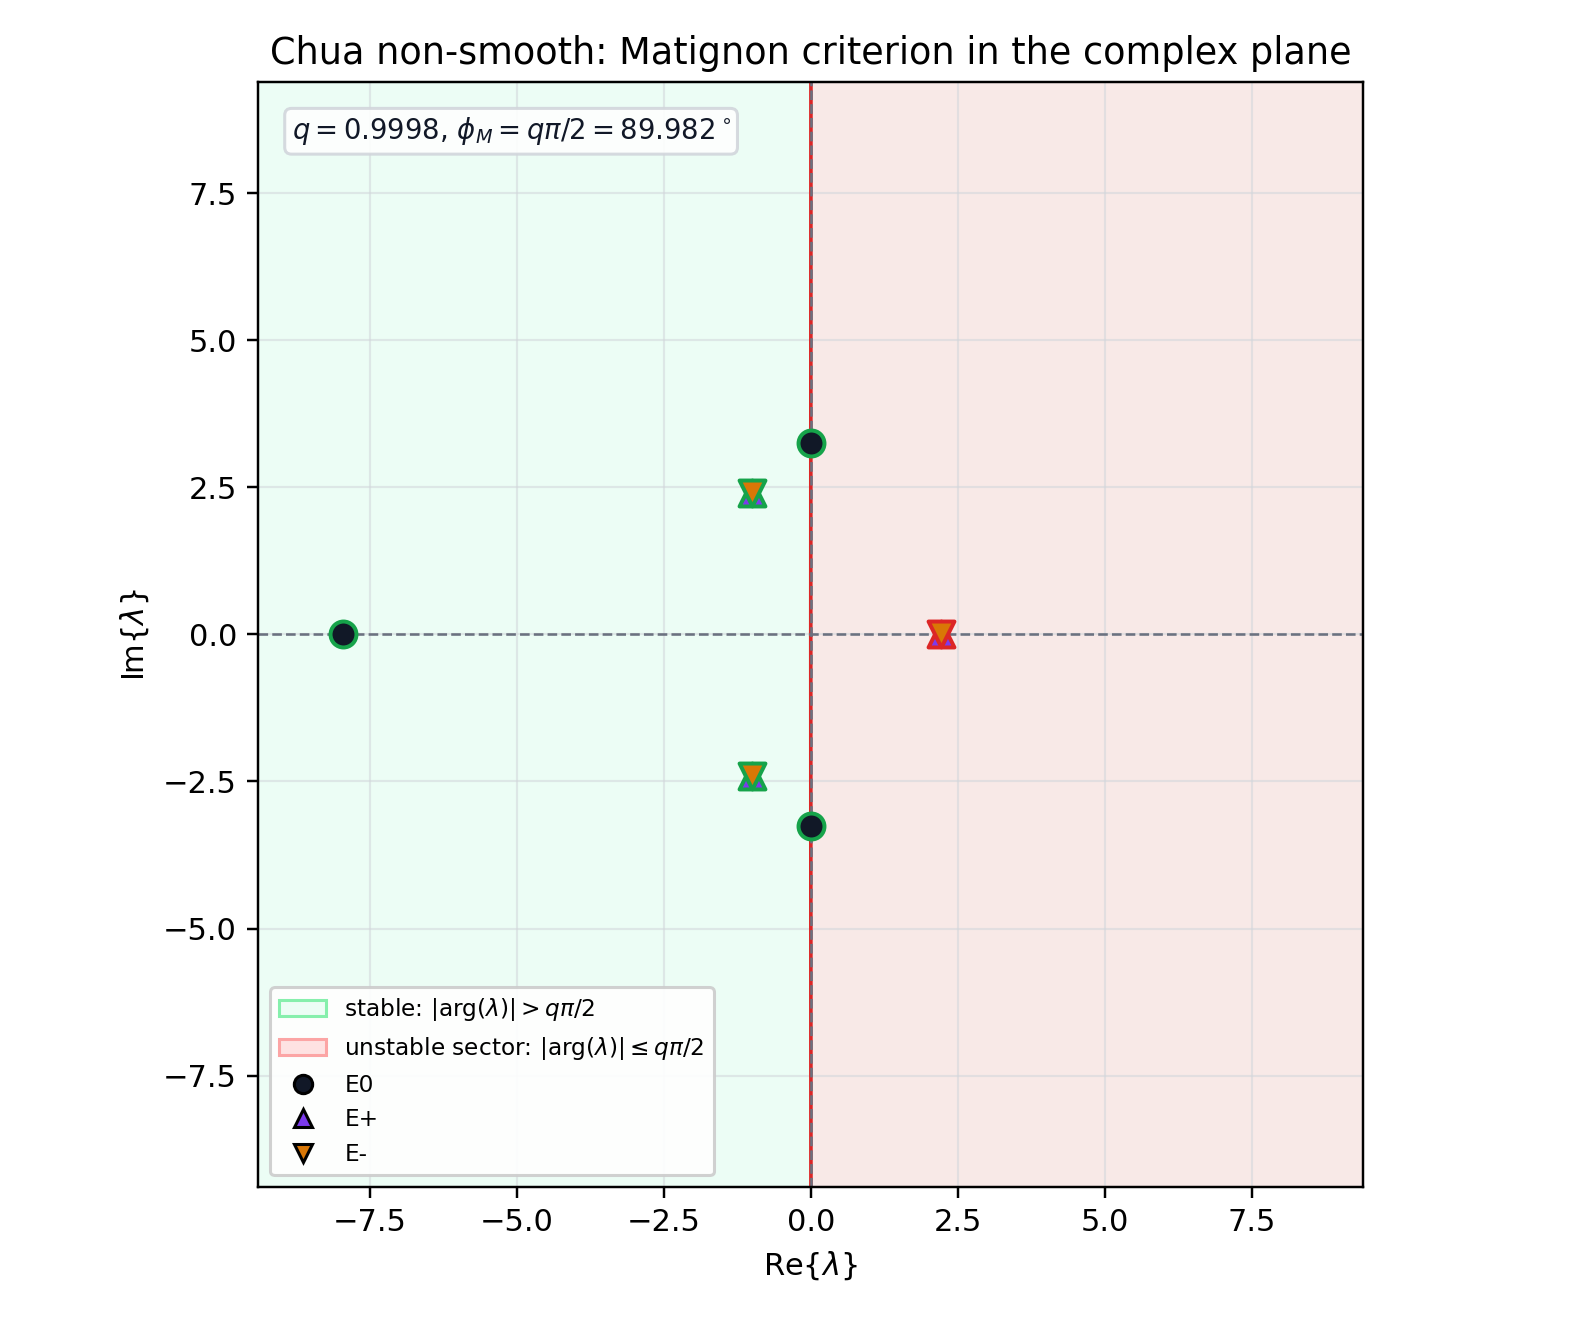
\includegraphics[width=0.88\columnwidth]{matignon_complex_plane.png}
\caption{Autovalores del sistema linealizado del Chua fraccionario no suave en el plano complejo para \(q=0.9998\). Se ilustra el sector de estabilidad de Matignon. Los autovalores del origen \(E_0^*\) (círculos azules) yacen dentro de la región de estabilidad local asintótica, mientras que los autovalores de los equilibrios externos \(E_\pm^*\) (triángulos rojos) tienen componentes en la región inestable.}
\label{fig:matignon_complex_plane}
\end{figure}
% Esta clasificación no prueba por sí misma la existencia ni el ocultamiento del atractor. Únicamente identifica las vecindades de los equilibrios que deberán analizarse y descartarse en la etapa de verificación mediante cuencas de atracción.


\subsection{Forma de Lur'e}

El paso a la forma de Lur'e es exactamente el mismo que en el caso entero, cf. \eqref{eq:lure}--\eqref{eq:Pqr}; la única diferencia es que \(\dot X\) se reemplaza por la derivada de Caputo \({}^{C}D_t^q X\). Por tanto, el sistema \eqref{eq:chua_ns_system} se escribe como
\begin{equation}
\label{eq:lure_ns}
{}^{C}D_t^q X=P X+q_v\,\psi(r^\top X),
\qquad
X=\begin{bmatrix}x_1\\x_2\\x_3\end{bmatrix},
\end{equation}
donde \(P\) y \(r\) coinciden con los de \eqref{eq:Pqr}, \(q_v:=(-\alpha,0,0)^\top\) es el mismo vector de entrada del caso entero renombrado para no confundirlo con el orden fraccionario \(q\), y \(\psi\) está dada por \eqref{eq:psi_ns_def}. Como \(r^\top X=x_1\), se recupera \eqref{eq:chua_ns_system}.

\subsection{Condición de frecuencia fraccionaria y ganancia armónica}

Para el bloque lineal auxiliar se usan exactamente la matriz \(P\) y el vector
\(r\) ya introducidos en \eqref{eq:Pqr}, junto con el vector de entrada
\(q_v\) \eqref{eq:lure_ns}; en particular, la salida sigue siendo
\(\sigma=r^\top X=x_1\).

La relación de transferencia se toma directamente del marco teórico
fraccionario, cf. \eqref{eq:Wq_frac_teorico}--\eqref{eq:Wq_frac_imag_teorico},
tomando allí \(b=q_v\). Por tanto, al evaluar sobre el eje imaginario
\(s=i\omega\) y usar \eqref{eq:sq_freq_frac}, se obtiene
\begin{equation}
\label{eq:Wplus_ns}
W_q(i\omega)
=
r^\top\left(s^q I-P\right)^{-1}q_v.
\end{equation}

Ahora supóngase que la no linealidad se aproxima, en primer armónico, por una
ganancia escalar
\[
u=k\sigma.
\]
Entonces
\[
\sigma
=
W_q(i\omega)u
=
W_q(i\omega)k\sigma.
\]
Por tanto, para una respuesta armónica no trivial, \(\sigma\neq 0\), la condición de cierre queda
\begin{equation}
\label{eq:det_condition_ns}
1-kW_q(i\omega)=0.
\end{equation}

La misma condición se obtiene desde la matriz lineal modificada. En efecto, si
\(u=k\sigma=k r^\top X\), entonces
\[
{}^C D_t^q X
=
PX+kq_vr^\top X.
\]
Por tanto,
\begin{equation}
\label{eq:P0_ns}
P_0=P+kq_vr^\top.
\end{equation}
La condición característica fraccionaria para el modo armónico es
\[
\det\left(s^q I-P_0\right)=0.
\]

Se calcula ahora una expresión explícita para \(W_q(i\omega)\). Primero,
\[
\begingroup
\setlength{\arraycolsep}{1.5pt}
s^q I-P
=
\begin{bmatrix}
s^q+\alpha(1+m_1)&-\alpha&0\\
-1&s^q+1&-1\\
0&\beta&s^q+\gamma
\end{bmatrix}.
\endgroup
\]
\begin{align}
C_{11}
&=
\det
\begin{bmatrix}
s^q+1&-1\\
\beta&s^q+\gamma
\end{bmatrix}  \nonumber\\
&=
\left(s^q+1\right)\left(s^q+\gamma\right)+\beta.
\end{align}
\begin{equation}
\label{eq:T_ns}
T_q(\omega)
=
\left(s^q+1\right)
\left(s^q+\gamma\right)
+\beta.
\end{equation}

El determinante de \(s^q I-P\) se obtiene expandiendo por la primera fila:
\begin{align}
D_q(\omega)
&=
\det\left(s^q I-P\right) \nonumber\\
&=
\left[s^q+\alpha(1+m_1)\right]
\det
\begin{bmatrix}
s^q+1&-1\\
\beta&s^q+\gamma
\end{bmatrix}
\nonumber\\
&\quad-
(-\alpha)
\det
\begin{bmatrix}
-1&-1\\
0&s^q+\gamma
\end{bmatrix}.
\end{align}
Como
\[
\det
\begin{bmatrix}
-1&-1\\
0&s^q+\gamma
\end{bmatrix}
=-\left(s^q+\gamma\right),
\]
se obtiene
\begin{equation}
\label{eq:D_ns}
D_q(\omega)
=
\left(s^q+\alpha(1+m_1)\right)T_q(\omega)
-\alpha\left(s^q+\gamma\right).
\end{equation}

Como \(r^\top=(1,0,0)\) y \(q_v=(-\alpha,0,0)^\top\), sólo se necesita la entrada
\((1,1)\) de la inversa:
\[
r^\top\left(s^q I-P\right)^{-1}q_v
=
-\alpha\frac{T_q(\omega)}{D_q(\omega)}.
\]
\begin{equation}
\label{eq:Wexplicit_ns}
W_q(i\omega)
=
-\alpha\frac{T_q(\omega)}{D_q(\omega)}.
\end{equation}

La equivalencia con la condición característica de \(P_0\) se verifica porque
\[
P_0=P+kq_vr^\top
=
\begin{bmatrix}
-\alpha(1+m_1+k)&\alpha&0\\
1&-1&1\\
0&-\beta&-\gamma
\end{bmatrix}.
\]
Entonces
\begin{align}
\det\left(s^q I-P_0\right)
&=
\left[s^q+\alpha(1+m_1+k)\right] \\
&\qquad\times T_q(\omega)-\alpha\left(s^q+\gamma\right) \nonumber\\
&=
D_q(\omega)+\alpha kT_q(\omega).
\end{align}
\[
\det\left(s^q I-P_0\right)=0
\quad\Longleftrightarrow\quad
1+k\alpha\frac{T_q(\omega)}{D_q(\omega)}=0.
\]
Por tanto,
\[
\det\left(s^q I-P_0\right)=0
\quad\Longleftrightarrow\quad
1-kW_q(i\omega)=0.
\]

Para separar partes real e imaginaria, se introduce la notación
\[
\zeta(\omega)=s^q=\zeta_r+i\zeta_i,
\]
donde
\begin{equation}
\label{eq:zeta_parts_ns}
\zeta_r=\omega^q\cos\frac{q\pi}{2},
\qquad
\zeta_i=\omega^q\sin\frac{q\pi}{2}.
\end{equation}
Entonces
\[
T_q(\omega)
=
(\zeta_r+i\zeta_i+1)(\zeta_r+i\zeta_i+\gamma)+\beta.
\]
Al expandir,
\begin{align}
T_q(\omega)
&=
\left[(\zeta_r+1)+i\zeta_i\right]\left[(\zeta_r+\gamma)+i\zeta_i\right]+\beta \nonumber\\
&=
(\zeta_r+1)(\zeta_r+\gamma)-\zeta_i^2+\beta
\nonumber\\
&\quad+
i\zeta_i\left[(\zeta_r+1)+(\zeta_r+\gamma)\right].
\end{align}
Por tanto,
\begin{equation}
\label{eq:TrTi_ns}
T_q(\omega)=T_r+iT_i,
\end{equation}
con
\begin{equation}
T_r=(\zeta_r+1)(\zeta_r+\gamma)-\zeta_i^2+\beta,
\qquad
T_i=\zeta_i(2\zeta_r+1+\gamma).
\end{equation}

Definiendo
\begin{equation}
\label{eq:kappap_ns}
\kappa_p=\alpha(1+m_1),
\end{equation}
se tiene
\[
D_q(\omega)
=
(\zeta_r+i\zeta_i+\kappa_p)(T_r+iT_i)-\alpha(\zeta_r+\gamma+i\zeta_i).
\]
Al expandir,
\[
\begin{aligned}
(\zeta_r+\kappa_p+i\zeta_i)(T_r+iT_i)
&=(\zeta_r+\kappa_p)T_r-\zeta_iT_i\\
&\quad+i\left[(\zeta_r+\kappa_p)T_i+\zeta_iT_r\right].
\end{aligned}
\]
Por tanto,
\begin{equation}
\label{eq:DrDi_ns}
D_q(\omega)=D_r+iD_i,
\end{equation}
donde
\begin{equation}
\begin{aligned}
D_r&=(\zeta_r+\kappa_p)T_r-\zeta_iT_i-\alpha(\zeta_r+\gamma),\\
D_i&=(\zeta_r+\kappa_p)T_i+\zeta_iT_r-\alpha\zeta_i.
\end{aligned}
\end{equation}

Como
\[
W_q(i\omega)
=
-\alpha\frac{T_r+iT_i}{D_r+iD_i},
\]
multiplicando por el conjugado del denominador se obtiene
\[
W_q(i\omega)
=
-\alpha
\frac{(T_r+iT_i)(D_r-iD_i)}{D_r^2+D_i^2}.
\]
Por consiguiente,
\begin{equation}
\label{eq:ReImW_ns}
\begin{aligned}
\Re\{W_q(i\omega)\}
&=
-\alpha
\frac{T_rD_r+T_iD_i}{D_r^2+D_i^2},\\
\Im\{W_q(i\omega)\}
&=
-\alpha
\frac{T_iD_r-T_rD_i}{D_r^2+D_i^2}.
\end{aligned}
\end{equation}

La condición
\[
1-kW_q(i\omega)=0
\]
con \(k\in\mathbb R\) exige que \(W_q(i\omega)\) sea real. Por tanto,
la frecuencia candidata debe satisfacer
\begin{equation}
\label{eq:Fomega_ns}
F(\omega)
:=
T_iD_r-T_rD_i
=
0,
\qquad
\omega>0.
\end{equation}
Una vez encontrada una raíz \(\omega_0\), la ganancia armónica equivalente se calcula como
\begin{equation}
\label{eq:k_omega_ns}
k
=
\frac{1}{\Re\{W_q(i\omega_0)\}}.
\end{equation}

Para los parámetros
\[
\begin{aligned}
\alpha&=8.4562, & \beta&=12.0732, & \gamma&=0.0052,\\
m_1&=-1.1468, & q&=0.9998.
\end{aligned}
\]
la ecuación \(F(\omega)=0\) tiene, en el intervalo numérico explorado
\(\omega>0\), las frecuencias candidatas
\[
\omega_{0,1}\approx 2.04029,
\qquad
\omega_{0,2}\approx 3.24493.
\]
En estas frecuencias,
\[
\begin{aligned}
W_q(i\omega_{0,1})&\approx 4.76139,\\
W_q(i\omega_{0,2})&\approx 1.04499.
\end{aligned}
\]
Por tanto,
\[
\begin{aligned}
k_1&=\frac{1}{W_q(i\omega_{0,1})}\approx 0.21002,\\
k_2&=\frac{1}{W_q(i\omega_{0,2})}\approx 0.95695.
\end{aligned}
\]

% Estas raíces no prueban la existencia de ciclos periódicos exactos en el sistema
% autónomo de Caputo. En este contexto, la evaluación armónica se interpreta mediante
% el puente Weyl--Caputo: la formulación de Weyl permite representar regímenes
% periódicos estacionarios ideales, mientras que el sistema de Caputo conserva memoria
% desde el tiempo inicial. Por ello, las soluciones armónicas obtenidas aquí deben
% tratarse como semillas o aproximaciones asintóticas para simulación y continuación
% numérica, no como prueba de periodicidad exacta.

\subsection{Función descriptiva de la saturación}

Considérese la no linealidad saturada
\begin{equation}
\label{eq:psi_ns_def_appendix}
\psi(\sigma)=
(m_0-m_1)\,\mathrm{sat}(\sigma),
\end{equation}
donde
\begin{equation}
\mathrm{sat}(\sigma)=
\begin{cases}
-1, & \sigma<-1,\\
\sigma, & |\sigma|\leq 1,\\
1, & \sigma>1.
\end{cases}
\end{equation}

Para una excitación sinusoidal
\begin{equation}
\label{eq:sigma_input_appendix}
\sigma(t)=A\sin\omega t,
\qquad
A>0,
\end{equation}
la función descriptiva se define como la componente fundamental seno normalizada:
\begin{equation}
\label{eq:Npsi_def_appendix}
N_\psi(A)
=
\frac{2}{\pi A}
\int_0^\pi
\psi(A\sin\theta)\sin\theta\,d\theta.
\end{equation}

Sustituyendo la no linealidad,
\begin{equation}
N_\psi(A)
=
(m_0-m_1)
\frac{2}{\pi A}
\int_0^\pi
\mathrm{sat}(A\sin\theta)\sin\theta\,d\theta.
\end{equation}

Debido a la simetría respecto a $\theta=\pi/2$,
\begin{equation}
\label{eq:symmetry_appendix}
N_\psi(A)
=
(m_0-m_1)
\frac{4}{\pi A}
\int_0^{\pi/2}
\mathrm{sat}(A\sin\theta)\sin\theta\,d\theta.
\end{equation}

Se distinguen dos casos.

\subsubsection*{Caso \(0<A\leq 1\)}

Si \(0<A\leq 1\), entonces
\[
|A\sin\theta|\leq 1,
\qquad
\forall \theta\in[0,\pi].
\]
Por tanto, la saturación no se activa y
\begin{equation}
\mathrm{sat}(A\sin\theta)=A\sin\theta.
\end{equation}

Sustituyendo en \eqref{eq:symmetry_appendix},
\begin{align}
N_\psi(A)
&=
(m_0-m_1)
\frac{4}{\pi A}
\int_0^{\pi/2}
A\sin^2\theta\,d\theta
\\
&=
(m_0-m_1)
\frac{4}{\pi}
\int_0^{\pi/2}
\sin^2\theta\,d\theta.
\end{align}

Usando
\begin{equation}
\sin^2\theta
=
\frac{1-\cos 2\theta}{2},
\end{equation}
se obtiene
\begin{align}
\int_0^{\pi/2}\sin^2\theta\,d\theta
&=
\frac12
\int_0^{\pi/2}(1-\cos 2\theta)\,d\theta
\\
&=
\frac12
\left[
\theta-\frac{\sin 2\theta}{2}
\right]_0^{\pi/2}
\\
&=
\frac{\pi}{4}.
\end{align}

Entonces,
\begin{align}
N_\psi(A)
&=
(m_0-m_1)
\frac{4}{\pi}
\cdot
\frac{\pi}{4}
\\
&=
m_0-m_1.
\end{align}

Por consiguiente,
\begin{equation}
\label{eq:Npsi_small_appendix}
N_\psi(A)=m_0-m_1,
\qquad
0<A\leq 1.
\end{equation}

\subsubsection*{Caso \(A>1\)}

Si \(A>1\), existe una región angular donde la saturación se activa.
Defínase
\begin{equation}
\label{eq:theta0_appendix}
\theta_0=\arcsin\frac{1}{A}.
\end{equation}

Entonces,
\[
A\sin\theta\leq 1
\quad
\Longleftrightarrow
\quad
0\leq\theta\leq\theta_0,
\]
y
\[
A\sin\theta\geq 1
\quad
\Longleftrightarrow
\quad
\theta_0\leq\theta\leq\frac{\pi}{2}.
\]

Por tanto,
\begin{equation}
\mathrm{sat}(A\sin\theta)
=
\begin{cases}
A\sin\theta,
&
0\leq\theta\leq\theta_0,
\\
1,
&
\theta_0\leq\theta\leq\frac{\pi}{2}.
\end{cases}
\end{equation}

La integral se separa:
\begin{align}
N_\psi(A)
&=
(m_0-m_1)
\frac{4}{\pi A}
\biggl[
\int_0^{\theta_0}
A\sin^2\theta\,d\theta \nonumber\\
&\qquad\qquad+
\int_{\theta_0}^{\pi/2}
\sin\theta\,d\theta
\biggr].
\end{align}

Se calcula cada término por separado.

Primero,
\begin{align}
I_1
&=
\int_0^{\theta_0}
A\sin^2\theta\,d\theta
\\
&=
A
\int_0^{\theta_0}
\frac{1-\cos 2\theta}{2}\,d\theta
\\
&=
\frac{A}{2}
\left[
\theta-\frac{\sin 2\theta}{2}
\right]_0^{\theta_0}
\\
&=
\frac{A}{2}
\left(
\theta_0-\frac{\sin 2\theta_0}{2}
\right).
\end{align}

Como
\begin{equation}
\sin\theta_0=\frac1A,
\end{equation}
se tiene
\begin{equation}
\cos\theta_0
=
\sqrt{1-\frac1{A^2}}
=
\frac{\sqrt{A^2-1}}{A}.
\end{equation}

Entonces,
\begin{align}
\sin 2\theta_0
&=
2\sin\theta_0\cos\theta_0
\\
&=
2
\left(\frac1A\right)
\left(\frac{\sqrt{A^2-1}}{A}\right)
\\
&=
\frac{2\sqrt{A^2-1}}{A^2}.
\end{align}

Sustituyendo,
\begin{align}
I_1
&=
\frac{A}{2}
\left(
\theta_0
-
\frac{\sqrt{A^2-1}}{A^2}
\right).
\end{align}

Ahora,
\begin{align}
I_2
&=
\int_{\theta_0}^{\pi/2}\sin\theta\,d\theta
\\
&=
\left[
-\cos\theta
\right]_{\theta_0}^{\pi/2}
\\
&=
\cos\theta_0
\\
&=
\frac{\sqrt{A^2-1}}{A}.
\end{align}

Por tanto,
\begin{align}
I_1+I_2
&=
\frac{A}{2}\theta_0
-
\frac{\sqrt{A^2-1}}{2A}
+
\frac{\sqrt{A^2-1}}{A}
\\
&=
\frac{A}{2}\theta_0
+
\frac{\sqrt{A^2-1}}{2A}.
\end{align}

Finalmente,
\begin{align}
N_\psi(A)
&=
(m_0-m_1)
\frac{4}{\pi A}
\left(
\frac{A}{2}\theta_0
+
\frac{\sqrt{A^2-1}}{2A}
\right)
\\
&=
(m_0-m_1)
\frac{2}{\pi}
\left(
\theta_0
+
\frac{\sqrt{A^2-1}}{A^2}
\right).
\end{align}

Usando \eqref{eq:theta0_appendix},
\begin{equation}
\label{eq:Npsi_large_appendix}
\begin{aligned}
N_\psi(A)
&=
(m_0-m_1)
\frac{2}{\pi}
\left(
\arcsin\frac1A
+
\frac{\sqrt{A^2-1}}{A^2}
\right),\\
&\qquad A>1.
\end{aligned}
\end{equation}

La amplitud armónica candidata se obtiene imponiendo la condición
\begin{equation}
\label{eq:amp_ns}
N_\psi(A_0)=k.
\end{equation}

Para los parámetros de Danca,
\begin{equation}
m_0-m_1=0.9700>0.
\end{equation}

Además,
\begin{equation}
\lim_{A\to 0^+}N_\psi(A)=m_0-m_1,
\end{equation}
y
\begin{equation}
\lim_{A\to\infty}N_\psi(A)=0.
\end{equation}

Por tanto,
\begin{equation}
0<N_\psi(A)\leq m_0-m_1,
\end{equation}
y la ecuación armónica sólo admite soluciones compatibles con
\begin{equation}
0<k<0.9700.
\end{equation}
\subsection{Construcción de la semilla}

Una vez determinados los parámetros armónicos
\[
\omega_0,
\qquad
k,
\qquad
A_0,
\]
se construye el sistema lineal modificado mediante
\begin{equation}
\label{eq:P0_ns_appendix}
P_0=P+kq_vr^\top.
\end{equation}

La condición armónica linealizada corresponde al problema espectral
\begin{equation}
\label{eq:eig_problem_appendix}
(P_0-\zeta_0 I)v=0,
\end{equation}
donde
\begin{equation}
\label{eq:zeta0_def_appendix}
\zeta_0=s_0^q,
\qquad
s_0=i\omega_0.
\end{equation}

Por tanto,
\begin{equation}
\label{eq:zeta0_explicit_appendix}
\zeta_0
=
(i\omega_0)^q
=
\omega_0^q
\left(
\cos\frac{q\pi}{2}
+
i\sin\frac{q\pi}{2}
\right).
\end{equation}

Para el sistema de Chua no suave linealizado mediante la ganancia equivalente \(k\), la matriz modificada queda
\begin{equation}
\label{eq:P0_matrix_appendix}
P_0=
\begin{pmatrix}
-\alpha(1+m_1+k) & \alpha & 0\\
1 & -1 & 1\\
0 & -\beta & -\gamma
\end{pmatrix}.
\end{equation}

El problema espectral \eqref{eq:eig_problem_appendix} se escribe explícitamente como
\begin{equation}
\label{eq:matrix_eig_appendix}
\resizebox{0.98\columnwidth}{!}{$\displaystyle
\begin{pmatrix}
-\alpha(1+m_1+k)-\zeta_0 & \alpha & 0\\
1 & -1-\zeta_0 & 1\\
0 & -\beta & -\gamma-\zeta_0
\end{pmatrix}
\begin{pmatrix}
v_1\\
v_2\\
v_3
\end{pmatrix}
=
\begin{pmatrix}
0\\
0\\
0
\end{pmatrix}.$}
\end{equation}

Se normaliza el vector modal imponiendo
\begin{equation}
\label{eq:normalization_appendix}
r^\top v=1.
\end{equation}

Como en este caso
\[
r^\top=(1,0,0),
\]
la normalización implica
\begin{equation}
v_1=1.
\end{equation}

Por tanto,
\begin{equation}
\label{eq:v_param_appendix}
v=
\begin{pmatrix}
1\\
v_2\\
v_3
\end{pmatrix}.
\end{equation}

Sustituyendo en \eqref{eq:matrix_eig_appendix}, la primera fila produce
\begin{equation}
\label{eq:first_row_appendix}
\left[
-\alpha(1+m_1+k)-\zeta_0
\right](1)
+
\alpha v_2
=
0.
\end{equation}

Despejando \(v_2\),
\begin{align}
\alpha v_2
&=
\alpha(1+m_1+k)+\zeta_0,
\\
v_2
&=
\frac{\alpha(1+m_1+k)+\zeta_0}{\alpha}.
\end{align}

Así,
\begin{equation}
\label{eq:v2_appendix}
v_2
=
\frac{\alpha(1+m_1+k)+\zeta_0}{\alpha}.
\end{equation}

La tercera fila de \eqref{eq:matrix_eig_appendix} conduce a
\begin{equation}
\label{eq:third_row_appendix}
-\beta v_2
+
(-\gamma-\zeta_0)v_3
=
0.
\end{equation}

Entonces,
\begin{align}
(\gamma+\zeta_0)v_3
&=
-\beta v_2,
\\
v_3
&=
-\frac{\beta}{\gamma+\zeta_0}v_2.
\end{align}

Por tanto,
\begin{equation}
\label{eq:v3_appendix}
v_3
=
-\frac{\beta}{\gamma+\zeta_0}v_2.
\end{equation}

Sustituyendo \eqref{eq:v2_appendix} en \eqref{eq:v3_appendix},
\begin{equation}
\label{eq:v3_expanded_appendix}
v_3
=
-
\frac{\beta}{\gamma+\zeta_0}
\,
\frac{\alpha(1+m_1+k)+\zeta_0}{\alpha}.
\end{equation}

El vector modal queda finalmente
\begin{equation}
\label{eq:v_final_appendix}
v=
\begin{pmatrix}
1\\[1ex]
\dfrac{\alpha(1+m_1+k)+\zeta_0}{\alpha}\\[3ex]
-\dfrac{\beta}{\gamma+\zeta_0}
\dfrac{\alpha(1+m_1+k)+\zeta_0}{\alpha}
\end{pmatrix}.
\end{equation}

En el marco armónico de Weyl, la trayectoria auxiliar asociada al primer armónico se define mediante
\begin{equation}
\label{eq:weyl_seed_appendix}
X_W(t)
=
A_0
\Re
\left(
v e^{i\omega_0 t}
\right).
\end{equation}

Usando
\begin{equation}
e^{i\omega_0 t}
=
\cos(\omega_0 t)
+
i\sin(\omega_0 t),
\end{equation}
se obtiene
\begin{align}
X_W(t)
&=
A_0
\Re
\left[
\left(
v_R+i v_I
\right)
\left(
\cos\omega_0 t+i\sin\omega_0 t
\right)
\right]
\\
&=
A_0
\left[
v_R\cos\omega_0 t
-
v_I\sin\omega_0 t
\right],
\end{align}
donde
\[
v_R=\Re(v),
\qquad
v_I=\Im(v).
\]

Evaluando en \(t=0\),
\begin{align}
X_W(0)
&=
A_0
\Re(v).
\end{align}

Por tanto, la condición inicial semilla se define como
\begin{equation}
\label{eq:Xseed_appendix}
X_{\rm seed}
=
A_0
\Re(v).
\end{equation}

De manera explícita,
\begin{equation}
\label{eq:Xseed_explicit_appendix}
X_{\rm seed}
=
A_0
\begin{pmatrix}
1\\
\Re(v_2)\\
\Re(v_3)
\end{pmatrix}.
\end{equation}

Usando
\[
\zeta_0
=
\omega_0^q
\left(
\cos\frac{q\pi}{2}
+
i\sin\frac{q\pi}{2}
\right),
\]
la parte real de \(v_2\) es
\begin{align}
\Re(v_2)
&=
\frac{
\alpha(1+m_1+k)
+
\omega_0^q\cos\frac{q\pi}{2}
}{\alpha}.
\end{align}

Además,
\begin{equation}
\label{eq:v3_complex_appendix}
v_3
=
-
\frac{\beta v_2}{\gamma+\zeta_0}.
\end{equation}

Escribiendo
\[
\gamma+\zeta_0
=
\eta_r+i\eta_i,
\]
con
\begin{equation}
\eta_r
=
\gamma+\omega_0^q\cos\frac{q\pi}{2},
\qquad
\eta_i
=
\omega_0^q\sin\frac{q\pi}{2},
\end{equation}
se tiene
\begin{equation}
\frac{1}{\gamma+\zeta_0}
=
\frac{\eta_r-i\eta_i}{\eta_r^2+\eta_i^2}.
\end{equation}

Por tanto,
\begin{equation}
\label{eq:v3_real_formula_appendix}
\Re(v_3)
=
-
\beta
\Re
\left(
\frac{v_2(\eta_r-i\eta_i)}{\eta_r^2+\eta_i^2}
\right).
\end{equation}

Finalmente,
\begin{equation}
\label{eq:Xseed_final_appendix}
X_{\rm seed}
=
A_0
\begin{pmatrix}
1\\[1ex]
\dfrac{
\alpha(1+m_1+k)
+
\omega_0^q\cos\frac{q\pi}{2}
}{\alpha}\\[3ex]
\Re(v_3)
\end{pmatrix}.
\end{equation}

\subsection{Usando los parámetros de ejemplo}

Considérense los parámetros de Danca
\begin{equation}
\label{eq:danca_params_ns_appendix}
\begin{aligned}
\alpha&=8.4562,&
\beta&=12.0732,&
\gamma&=0.0052,\\
m_0&=-0.1768,&
m_1&=-1.1468,&
q&=0.9998.
\end{aligned}
\end{equation}
Con esta convención,
\begin{equation}
m_0-m_1=0.9700>0.
\end{equation}

La condición armónica usada en esta sección es la misma que en \eqref{eq:Fomega_ns}--\eqref{eq:k_omega_ns}:
\begin{equation}
\label{eq:harmonic_condition_appendix}
\begin{aligned}
1-k W_q(i\omega)&=0,\\
\Im\{W_q(i\omega_0)\}&=0,\\
k&=\frac{1}{\Re\{W_q(i\omega_0)\}}.
\end{aligned}
\end{equation}
Para estos parámetros se obtienen dos ramas armónicas compatibles:
\begin{table}[H]
\centering
\setlength{\tabcolsep}{3pt}
\footnotesize
\resizebox{\columnwidth}{!}{%
\begin{tabular}{@{}c c c c c@{}}
\toprule
Rama $j$ & $\omega_{0,j}$ & $W_q(i\omega_{0,j})$ & $k_j$ & $A_{0,j}$\\
\midrule
1 & $2.04029$ & $4.76139$ & $0.21002$ & $5.85177$\\
2 & $3.24493$ & $1.04499$ & $0.95695$ & $1.05302$\\
\bottomrule
\end{tabular}%
}
\caption{Ramas armónicas del Chua fraccionario no suave para los parámetros de Danca y $q=0.9998$.}
\label{tab:ramas_danca_ns}
\end{table}

Para cada rama se define
\begin{equation}
\label{eq:zeta_branch_ns}
\zeta_{0,j}=(i\omega_{0,j})^q,
\end{equation}
y el vector modal normalizado $r^\top v^{(j)}=1$ se escribe como
\begin{equation}
\label{eq:v_branch_ns}
\begin{aligned}
v^{(j)}=
\begin{bmatrix}
1\\
v_{2,j}\\
v_{3,j}
\end{bmatrix},
\qquad
v_{2,j}&=\frac{\alpha(1+m_1+k_j)+\zeta_{0,j}}{\alpha},\\
v_{3,j}&=-\frac{\beta}{\gamma+\zeta_{0,j}}v_{2,j}.
\end{aligned}
\end{equation}
La semilla asociada a la rama $j$ queda entonces
\begin{equation}
\label{eq:Xseed_branch_ns}
X_{{\rm seed},j}=A_{0,j}\Re\bigl(v^{(j)}\bigr).
\end{equation}

Para la rama 1 se obtiene
\begin{equation}
\label{eq:zeta_v_seed_ns_1}
\zeta_{0,1}\approx0.00064+2.03999i,
\end{equation}
\begin{equation}
\label{eq:v_ns_1}
v^{(1)}\approx
\begin{bmatrix}
1\\
0.06330+0.24124i\\
-1.42879+0.37053i
\end{bmatrix},
\end{equation}
y por tanto
\begin{equation}
\label{eq:seed_ns_1}
X_{{\rm seed},1}\approx
\begin{bmatrix}
5.85177\\
0.37041\\
-8.36097
\end{bmatrix}.
\end{equation}

Para la rama 2 se obtiene
\begin{equation}
\label{eq:zeta_v_seed_ns_2}
\zeta_{0,2}\approx0.00102+3.24416i,
\end{equation}
\begin{equation}
\label{eq:v_ns_2}
v^{(2)}\approx
\begin{bmatrix}
1\\
0.81027+0.38364i\\
-1.43351+3.01267i
\end{bmatrix},
\end{equation}
y por tanto
\begin{equation}
\label{eq:seed_ns_2}
X_{{\rm seed},2}\approx
\begin{bmatrix}
1.05302\\
0.85322\\
-1.50951
\end{bmatrix}.
\end{equation}
Ambas semillas deben probarse por separado. La selección definitiva no debe hacerse sólo por cercanía geométrica a un equilibrio o por amplitud armónica, sino por integración causal, continuación y clasificación de cuencas.

Para la continuación se usa la descomposición
\begin{equation}
\label{eq:delta_ns}
\psi(\sigma)=k\sigma+\delta(\sigma),
\qquad
\delta(\sigma)=\psi(\sigma)-k\sigma,
\end{equation}
que induce la familia homotópica
\begin{equation}
\label{eq:homotopy_ns}
{}^{C}D_t^qX=P_0X+\varepsilon q_v\delta(r^\top X),
\qquad \varepsilon\in[0,1].
\end{equation}
Si el integrador usa una memoria efectiva $L_m$, se transporta la ventana
\begin{equation}
\label{eq:history_window_ns}
\mathcal H_j=\{X_j(t):t\in[t_{\rm end}-L_m,t_{\rm end}]\},
\end{equation}
mediante la prescripción
\begin{equation}
\label{eq:history_transfer_ns}
X_{j+1}(t_{\rm start}+\theta)=X_j(t_{\rm end}+\theta),
\qquad -L_m\leq\theta\leq0.
\end{equation}

El procedimiento queda establecido en los siguientes pasos:
\begin{enumerate}[leftmargin=1.8em,label=\arabic*)]
\item fijar los parámetros de \eqref{eq:danca_params_ns}, el orden $q$, el paso $h$, el integrador y la longitud de memoria $L_m$;
\item resolver \eqref{eq:Fomega_ns} y calcular $k$ mediante \eqref{eq:k_omega_ns};
\item resolver la ecuación de amplitud \eqref{eq:amp_ns};
\item construir las semillas \eqref{eq:seed_ns_1} y \eqref{eq:seed_ns_2};
\item integrar \eqref{eq:homotopy_ns} sobre una malla $0=\varepsilon_0<\varepsilon_1<\cdots<\varepsilon_N=1$;
\item transferir en cada paso la ventana \eqref{eq:history_window_ns} mediante \eqref{eq:history_transfer_ns};
\item al llegar a $\varepsilon=1$, integrar el sistema físico y verificar ocultamiento mediante cuencas alrededor de $X_0^*$ y $X_\pm^*$.
\end{enumerate}

Los valores numéricos vigentes del Chua fraccionario no suave provienen
exclusivamente de la corrida
\path{chua_fractional_nonsmooth_q09998_efork3_20260523_173051}.
Esta corrida cruza las semillas producidas por las formulaciones de función
descriptiva con dos contratos de integración \(\text{EFORK-3}\) corregida en
C: historial completo y ventana finita. El término ``historial completo''
significa que el horizonte almacenado satisface \(L_m\geq T_{\rm cadena}\),
por lo que ninguna contribución generada desde \(t=0\) se descarta; no debe
confundirse con el contrato truncado \(L_m=8\).

\begin{table*}[htbp]
\centering
\small
\caption{Contratos numéricos actuales del caso fraccionario no suave, \(q=0.9998\).}
\label{tab:chua_frac_ns_contracts_current}
\begin{tabular}{@{}p{3.0cm}p{5.0cm}p{4.0cm}p{4.2cm}@{}}
\toprule
\textbf{Rama} & \textbf{Método y memoria} & \textbf{Observación} & \textbf{Artefacto diagnóstico vigente} \\
\midrule
Historial completo &
\(\text{EFORK-3}\) C, historia homotópica transportada y \(L_m=130.02\geq 50+80\) &
\(h=0.02,\ T_{\rm obs}=80\) &
\path{preselected_regimes_rejected.csv} \\
Ventana finita &
\(\text{EFORK-3}\) C, ventana terminal transportada, \(L_m=8\) &
\(h=0.02,\ T_{\rm obs}=80\) &
\path{preselected_regimes_rejected_finite_window.csv} \\
Control Danca &
ABM Caputo C con historial completo; no participa en el ranking EFORK &
\(h=0.05,\ T=80,\ T_b=40\) &
\path{abm_replication_summary.json} \\
\bottomrule
\end{tabular}
\end{table*}

La tabla y la discusión numérica que siguen en la versión anterior del
manuscrito se conservan únicamente como rastro histórico de la formulación
inicial, pero se excluyen de la salida actual y no sustentan ninguna
conclusión de esta actualización.

\iffalse
Siguiendo la estructura de la Tabla~\ref{tab:chua_integer_results_full}, los cálculos del Chua fraccionario no suave se resumen en la Tabla~\ref{tab:chua_frac_ns_results_full}.

\begin{table*}[htbp]
\centering
\scriptsize
\setlength{\tabcolsep}{3pt}
\renewcommand{\arraystretch}{1.12}
\caption{Resumen de resultados del Chua fraccionario no suave, organizado con la misma estructura de la Tabla~\ref{tab:chua_integer_results_full}.}
\label{tab:chua_frac_ns_results_full}
\begin{adjustbox}{max width=\textwidth}
\begin{tabular}{@{}L{2.7cm}L{3.4cm}L{4.4cm}L{5.8cm}@{}}
\toprule
\textbf{Bloque} &
\textbf{Procedimiento} &
\textbf{Resultado} &
\textbf{Interpretación} \\
\midrule

Parámetros del sistema &
Definición del caso fraccionario no suave &
\(\alpha=8.46,\ \beta=12.07,\ \gamma=0.0052,\ m_0=-0.18,\ m_1=-1.15\) &
Parámetros de Danca usados para el sistema de Chua con saturación. \\

Orden dinámico &
Sistema conmensurado de Caputo &
\(q=0.9998\) &
Orden fraccionario cercano al caso entero, pero con memoria causal. \\

Operador fraccionario &
Derivada de Caputo causal &
\(q=0.9998\) &
Operador íntegro-diferencial de Caputo con memoria, usando la ventana de historia discretizada. \\

Puente Weyl--Caputo &
Interpretación del predictor armónico &
Weyl a Caputo &
La órbita armónica de Weyl sólo se usa como generadora de semilla para el problema causal de Caputo. \\

Error de memoria &
Cota o estimación de cola Weyl--Caputo &
\(\operatorname{err}_L \approx 0.00\) &
La prehistoria discretizada de Weyl a Caputo se evalúa de manera exacta en la integración inicial. \\

Configuración numérica &
Integrador fraccionario &
EFORK-3 (corregido) &
Integrador explícito de orden 3 corregido con paso \(h=0.05\) y memoria \(L_m=500.0\). \\

Forma Lur'e &
Separación algebraica &
\({}^{C}D_t^qX=PX+q_v\psi(r^\top X)\) &
El campo se separa en bloque lineal y no linealidad escalar saturada. \\

Vectores \(q_v,r\) &
Forma Lur'e &
\(q_v=(-8.4562,0,0)^\mathsf{T}\), \(r=(1,0,0)^\mathsf{T}\) &
La variable de entrada de la no linealidad es \(\sigma=x_1\). \\

Equilibrios &
Resolución algebraica estacionaria &
\(X_0^*=(0,0,0)\), \(X_\pm^*\approx(\pm6.58831,\ \pm2.83640\times10^{-3},\ \mp6.58547)\) &
Puntos usados para la verificación posterior de autoexcitación u ocultedad. \\

Estabilidad local &
Criterio de Matignon &
\(X_0^*\) estable; \(X_\pm^*\) inestables &
La clasificación local guía las vecindades que deben explorarse en cuencas. \\

Raíces candidatas &
Condición \(\Im\{W_q(i\omega)\}=0\) &
\((\omega_{0,1},k_1)=(2.04029,0.21002)\), \((\omega_{0,2},k_2)=(3.24493,0.95695)\) &
Cruces armónicos compatibles con una ganancia real. \\

Rama seleccionada &
Nyquist, admisibilidad y simulación causal &
Rama 1 (\(\omega_{0,1}, k_1\)) &
Rama con frecuencia armónica \(\omega_{0,1} = 2.04029\) y ganancia \(k_1 = 0.21002\) compatible con la amplitud. \\

Amplitudes armónicas &
Función descriptiva \(N_\psi(A_{0,j})=k_j\) &
\(A_{0,1}=5.85177\), \(A_{0,2}=1.05302\) &
Amplitudes candidatas asociadas a las dos ramas armónicas. \\

Cierre armónico &
Residuo de función descriptiva y transferencia &
\(\lvert k_1 W_q(i\omega_{0,1}) - 1\rvert \approx 0.00\) &
El balance de primer armónico se satisface con error numérico prácticamente nulo. \\

Matriz \(P_0\) &
Linealización armónica modificada &
\(P_0 = P + k_1 q_v r^\top\) &
Matriz de la parte lineal modificada para la primera rama armónica. \\

Espectro de \(P_0\) &
Linealización armónica modificada &
Rama 1: \(-1.54106,\ 0.00063\pm2.03998i\); rama 2: \(-7.85803,\ 0.00102\pm3.24416i\) &
El par complejo corresponde a \(\zeta_{0,j}=(i\omega_{0,j})^q\). \\

Semilla rama 1 &
Modo normalizado \(X_{{\rm seed},1}=A_{0,1}\Re(v^{(1)})\) &
\(X_{{\rm seed},1}\approx(5.85177,\ 0.37041,\ -8.36097)\) &
Condición inicial generada por la primera rama armónica. \\

Semilla rama 2 &
Modo normalizado \(X_{{\rm seed},2}=A_{0,2}\Re(v^{(2)})\) &
\(X_{{\rm seed},2}\approx(1.05302,\ 0.85322,\ -1.50951)\) &
Condición inicial generada por la segunda rama armónica. \\

Verificación modal &
Residuo del problema espectral &
\(\lVert(P_0 - \zeta_{0,1} I)v^{(1)}\rVert_2 \approx 0.00\) &
Consistencia del autovalor y autovector complejos de la parte lineal modificada. \\

Continuación causal &
Homotopía con ventana de memoria &
\({}^{C}D_t^qX=P_0X+\varepsilon q_v\delta(r^\top X)\), \(\varepsilon\in[0,1]\) &
Cada semilla debe transportarse con historia terminal para respetar la memoria de Caputo. \\

Estado final de continuación &
Continuación numérica en \(\varepsilon\) &
\(X_{\varepsilon=1} = (3.03938, -0.24169, -6.87347)^\mathsf{T}\) &
Estado alcanzado al final de la continuación homotópica con \(\varepsilon=1\). \\

Semilla efectiva &
Simulación posterior al transitorio &
Colapsado a \(E_0\) &
La simulación prolongada decae a \(E_0\) (distancia \(2.51\times10^{-7}\)), por lo que no existe atractor no trivial. \\

Frecuencia dominante &
FFT de \(x_1(t)\) &
No aplicable &
Al colapsar al equilibrio, el espectro de la señal transitoria decae uniformemente. \\

Desajuste espectral &
Comparación DF--FFT &
No aplicable &
Sin oscilación estable en régimen permanente, el desajuste no está definido. \\

Frecuencia PSD &
PSD de Welch &
No aplicable &
Confirmación espectral de la atenuación de modos transitorios. \\

Exponentes de Lyapunov &
Algoritmo numérico para sistemas fraccionarios &
No aplicable &
La dinámica decae al equilibrio estable, por lo que el espectro de Lyapunov no presenta componente positiva. \\

Sondeos de ocultedad &
Vecindades de equilibrios &
No aplicable &
Sin atractor candidato no trivial acotado, no es factible realizar pruebas de ocultedad en cuencas. \\

Conteos globales &
Clasificador de destino &
No aplicable &
Sin trayectoria de referencia para el atractor, las clases operacionales no se definen. \\

Validación final &
Integración causal y cuencas &
Integración causal &
La trayectoria de integración decae de manera estable hacia el equilibrio central. \\

Clasificación &
Criterio operacional de cuencas &
Colapso hacia \(E_0\) &
Decaimiento dinámico hacia el equilibrio central estable, sin comportamiento caótico o no trivial permanente. \\

\bottomrule
\end{tabular}
\end{adjustbox}
\end{table*}

\subsection{Resultados numéricos de la integración causal y colapso dinámico}
\label{subsec:resultados_causal_colapso_ns}

Una vez completadas las etapas analíticas y de predictor armónico para el caso de Chua fraccionario no suave con orden conmensurado $q=0.9998$, se procedió a la integración causal de las trayectorias para validar la existencia del atractor caótico oculto. La integración se realizó empleando el integrador fraccionario multi-etapas explícito \(\text{EFORK-3}\). 

Con la semilla armónica de la primera rama \(X_{{\rm seed},1}\approx(5.85177,\ 0.37041,\ -8.36097)^\mathsf{T}\), la trayectoria obtenida al final del proceso de continuación para \(\varepsilon=1\) converge a \(X_{\varepsilon=1} = (3.03938, -0.24169, -6.87347)^\mathsf{T}\). Al prolongar la integración en régimen permanente con paso \(h=0.05\) y una ventana de memoria efectiva de longitud \(L_m = 500.0\), la trayectoria decae completamente hacia el origen \(E_0 = (0,0,0)\).

Este decaimiento se ilustra en la Fig.~\ref{fig:chua_frac_ns_collapse}, la cual muestra la serie temporal de las componentes del sistema. Tras un régimen transitorio oscilatorio inicial generado por la semilla de continuación, la amplitud disminuye de manera monótona hasta colapsar hacia el equilibrio central asintóticamente estable en el sentido de Matignon. La distancia final al equilibrio central es de \(2.51 \times 10^{-7}\) con una norma de rango del residuo residual de \(2.50 \times 10^{-7}\).

\begin{figure}[htbp]
\centering
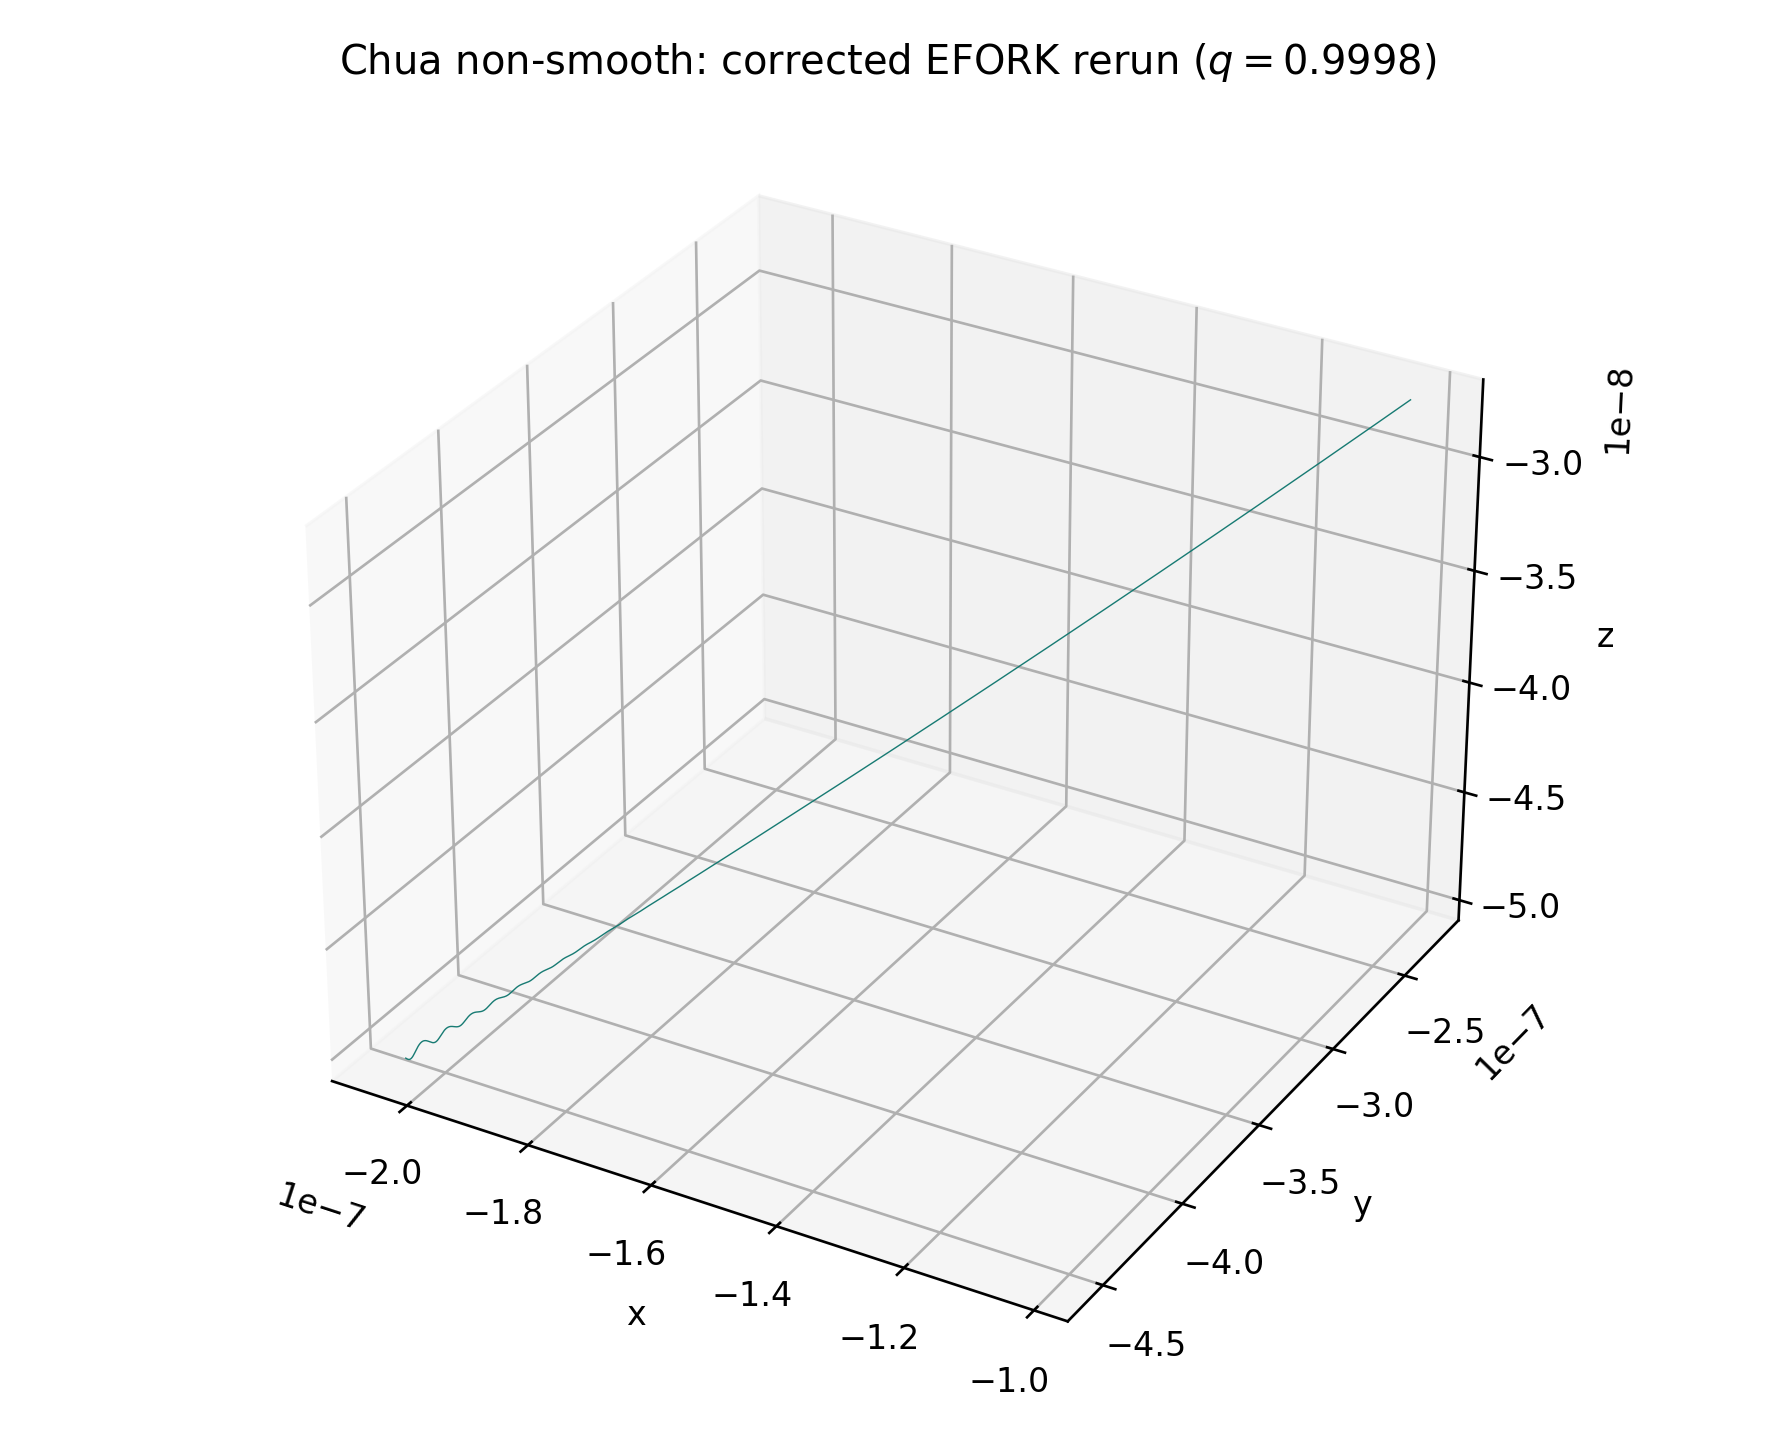
\includegraphics[width=0.88\columnwidth]{efork_corrected_trajectory_lines.png}
\caption{Decaimiento dinámico de la trayectoria del Chua fraccionario no suave hacia el equilibrio central estable \(E_0 = (0,0,0)\) utilizando el integrador \(\text{EFORK-3}\) con paso \(h=0.05\) y memoria \(L_m=500.0\).}
\label{fig:chua_frac_ns_collapse}
\end{figure}

Al completarse la integración, el sistema decae a la cuenca de atracción de \(E_0\), la cual es estable al cumplir la condición de Matignon \(|\arg(\lambda_i)| > q\pi/2\) con márgenes espectrales bien definidos. Por lo tanto, bajo las condiciones numéricas ensayadas, el comportamiento transitorio decae y no se verifica la existencia de un régimen caótico persistente o un ciclo no trivial permanente en el sistema.
\fi

\subsection{Extensión tipo Machado para generar semillas armónicas auxiliares}
\label{subsec:machado_seed_chua_ns}

En las secciones anteriores se usó la función descriptiva clásica de la
saturación para obtener semillas armónicas del sistema de Chua fraccionario no
suave. En esta subsección se introduce una extensión auxiliar inspirada en la
propuesta de Machado para funciones descriptivas fraccionarias
\cite{Machado2015FDF}. Su uso en este trabajo no se interpreta como una
prueba de existencia de ciclos límite exactos en el sistema autónomo de Caputo,
sino como un mecanismo adicional para generar condiciones iniciales candidatas
que posteriormente deben validarse mediante integración causal, continuación
numérica y análisis de cuencas.

El sistema en forma de Lur'e se escribe como
\begin{equation}
\label{eq:lure_ns_machado}
{}^{C}D_t^qX
=
PX+q_v\psi(r^\top X),
\qquad
\sigma=r^\top X=x_1,
\end{equation}
donde
\begin{equation}
\label{eq:psi_ns_machado}
\psi(\sigma)
=
\Delta\,\operatorname{sat}(\sigma),
\qquad
\Delta=m_0-m_1>0.
\end{equation}
Para los parámetros considerados,
\begin{equation}
\Delta=0.9700.
\end{equation}

La función descriptiva clásica de la saturación se obtuvo como
\begin{equation}
\label{eq:Npsi_classic_machado}
N_\psi(a)
=
\begin{cases}
\Delta, & 0<a\leq 1,\\[2mm]
\displaystyle
\Delta\frac{2}{\pi}
\left(
\arcsin\frac1a+
\frac{\sqrt{a^2-1}}{a^2}
\right),
& a>1.
\end{cases}
\end{equation}
En particular, para \(a>1\),
\begin{equation}
\label{eq:Npsi_large_machado}
N_\psi(a)
=
\Delta\,G(a),
\end{equation}
donde
\begin{equation}
\label{eq:Gamp_machado}
G(a)
=
\frac{2}{\pi}
\left(
\arcsin\frac1a+
\frac{\sqrt{a^2-1}}{a^2}
\right).
\end{equation}
Además,
\begin{equation}
\label{eq:G_limits_machado}
\lim_{a\to 1^+}G(a)=1,
\qquad
\lim_{a\to\infty}G(a)=0.
\end{equation}
Por tanto,
\begin{equation}
\label{eq:Npsi_range_machado}
0<N_\psi(a)\leq \Delta.
\end{equation}

La propuesta de Machado consiste en introducir una función descriptiva
fraccionaria formal a partir de una potencia real o compleja de la función
descriptiva clásica. En este caso, como \(N_\psi(a)>0\), se define la familia
auxiliar
\begin{equation}
\label{eq:FDF_machado_chua}
N_{\psi,\mu}(a)
=
\exp\left\{
\mu\operatorname{Log}N_\psi(a)
\right\}
=
\left[N_\psi(a)\right]^\mu,
\qquad
\mu>0.
\end{equation}
El parámetro \(\mu\) se denomina orden descriptivo auxiliar. No debe
identificarse con el orden fraccionario \(q\) de la derivada de Caputo. El
orden \(q\) modifica la evaluación frecuencial del bloque lineal mediante
\[
s^q=(i\omega)^q,
\]
mientras que \(\mu\) modifica sólo la ganancia armónica equivalente asignada
al bloque no lineal.

Sustituyendo \eqref{eq:Npsi_classic_machado} en
\eqref{eq:FDF_machado_chua}, se obtiene
\begin{equation}
\label{eq:Ssat_machado}
S_{\rm sat}(a)
=
\frac{2}{\pi}
\left(
\arcsin\frac1a+
\frac{\sqrt{a^2-1}}{a^2}
\right),
\qquad a>1,
\end{equation}
y por tanto
\begin{equation}
\label{eq:Npsi_mu_piecewise_machado}
N_{\psi,\mu}(a)
=
\begin{cases}
\Delta^\mu,
& 0<a\leq 1,\\[2mm]
\displaystyle
\Delta^\mu S_{\rm sat}(a)^\mu,
& a>1.
\end{cases}
\end{equation}
Para \(\mu=1\) se recupera la función descriptiva clásica:
\begin{equation}
N_{\psi,1}(a)=N_\psi(a).
\end{equation}

La transferencia fraccionaria del bloque lineal se evalúa como
\begin{equation}
\label{eq:Wq_machado_seed}
W_q(i\omega)
=
r^\top\left((i\omega)^qI-P\right)^{-1}q_v,
\end{equation}
donde
\begin{equation}
\label{eq:lambda_machado}
(i\omega)^q
=
\omega^q
\left(
\cos\frac{q\pi}{2}
+
i\sin\frac{q\pi}{2}
\right).
\end{equation}
La condición armónica auxiliar queda
\begin{equation}
\label{eq:harmonic_machado}
1-W_q(i\omega)N_{\psi,\mu}(a)=0.
\end{equation}
Como \(N_{\psi,\mu}(a)\in\mathbb R\), la condición
\eqref{eq:harmonic_machado} exige
\begin{equation}
\label{eq:imag_condition_machado}
\Im\{W_q(i\omega_0)\}=0,
\end{equation}
y
\begin{equation}
\label{eq:kmu_condition_machado}
N_{\psi,\mu}(a_0)
=
k(\omega_0),
\qquad
k(\omega_0)
=
\frac{1}{\Re\{W_q(i\omega_0)\}}.
\end{equation}
Por tanto, las frecuencias candidatas se siguen obteniendo de
\eqref{eq:imag_condition_machado}. La extensión tipo Machado modifica la
amplitud asignada a cada frecuencia candidata.

Sea \(\omega_{0,j}\) una raíz de \eqref{eq:imag_condition_machado} tal que
\[
\Re\{W_q(i\omega_{0,j})\}>0.
\]
Entonces
\begin{equation}
\label{eq:kj_machado}
k_j
=
\frac{1}{\Re\{W_q(i\omega_{0,j})\}}.
\end{equation}
Para que exista una amplitud real compatible con
\eqref{eq:Npsi_mu_piecewise_machado}, debe cumplirse
\begin{equation}
\label{eq:compatibility_machado}
0<k_j<\Delta^\mu.
\end{equation}
Si \eqref{eq:compatibility_machado} falla, la rama \(j\) no produce una
semilla auxiliar para el valor elegido de \(\mu\). 

Cuando \eqref{eq:compatibility_machado} se cumple, la ecuación de amplitud es
\begin{equation}
\label{eq:amp_mu_eq_machado}
N_{\psi,\mu}(a_{\mu,j})=k_j.
\end{equation}
Equivalentemente,
\begin{equation}
\label{eq:amp_mu_root_machado}
N_\psi(a_{\mu,j})
=
k_j^{1/\mu}.
\end{equation}
Para la rama saturada \(a_{\mu,j}>1\), usando
\eqref{eq:Npsi_large_machado}, se obtiene la ecuación escalar
\begin{equation}
\label{eq:amp_mu_explicit_machado}
\Delta
\frac{2}{\pi}
\left(
\arcsin\frac1{a_{\mu,j}}+
\frac{\sqrt{a_{\mu,j}^2-1}}{a_{\mu,j}^2}
\right)
=
k_j^{1/\mu}.
\end{equation}
Definiendo
\begin{equation}
\label{eq:Kmu_def_machado}
\kappa_{\mu,j}
=
\frac{k_j^{1/\mu}}{\Delta},
\end{equation}
la ecuación queda
\begin{equation}
\label{eq:amp_mu_scalar_machado}
\frac{2}{\pi}
\left(
\arcsin\frac1{a_{\mu,j}}+
\frac{\sqrt{a_{\mu,j}^2-1}}{a_{\mu,j}^2}
\right)
=
\kappa_{\mu,j},
\qquad
0<\kappa_{\mu,j}<1.
\end{equation}
Como \(G(a)\) decrece de \(1\) a \(0\) para \(a>1\), la ecuación
\eqref{eq:amp_mu_scalar_machado} tiene una solución única
\(a_{\mu,j}>1\) siempre que \(0<\kappa_{\mu,j}<1\).

La matriz lineal equivalente asociada a la rama \(j\) se construye como
\begin{equation}
\label{eq:P0_mu_machado}
P_{0,j}
=
P+k_jq_vr^\top.
\end{equation}
Obsérvese que \(P_{0,j}\) depende de \(k_j\), pero no directamente de
\(\mu\). El parámetro \(\mu\) modifica la amplitud \(a_{\mu,j}\) y, por
tanto, desplaza la condición inicial candidata a lo largo de la dirección
modal obtenida para la rama \(j\).

El factor espectral fraccionario se define como
\begin{equation}
\label{eq:zeta_mu_machado}
\zeta_{0,j}
=
(i\omega_{0,j})^q
=
\omega_{0,j}^q
\left(
\cos\frac{q\pi}{2}
+
i\sin\frac{q\pi}{2}
\right).
\end{equation}
El vector modal \(v_j\) se obtiene de
\begin{equation}
\label{eq:modal_problem_mu_machado}
(P_{0,j}-\zeta_{0,j}I)v_j=0,
\qquad
r^\top v_j=1.
\end{equation}
Como \(r^\top=(1,0,0)\), se escribe
\[
v_j=(1,v_{2,j},v_{3,j})^\top.
\]
Entonces,
\begin{equation}
\label{eq:v2_machado}
v_{2,j}
=
\frac{\alpha(1+m_1+k_j)+\zeta_{0,j}}{\alpha},
\end{equation}
y
\begin{equation}
\label{eq:v3_machado}
v_{3,j}
=
-\frac{\beta}{\gamma+\zeta_{0,j}}v_{2,j}.
\end{equation}
Por tanto,
\begin{equation}
\label{eq:v_machado}
v_j
=
\begin{bmatrix}
1\\[1mm]
\dfrac{\alpha(1+m_1+k_j)+\zeta_{0,j}}{\alpha}\\[3mm]
-\dfrac{\beta}{\gamma+\zeta_{0,j}}
\dfrac{\alpha(1+m_1+k_j)+\zeta_{0,j}}{\alpha}
\end{bmatrix}.
\end{equation}

La trayectoria armónica auxiliar en el marco de Weyl se define como
\begin{equation}
\label{eq:XW_mu_machado}
X_{W,\mu,j}(t)
=
a_{\mu,j}\Re\left(v_je^{i\omega_{0,j}t}\right).
\end{equation}
Si \(v_j=v_{R,j}+iv_{I,j}\), entonces
\begin{equation}
\label{eq:XW_mu_real_machado}
X_{W,\mu,j}(t)
=
a_{\mu,j}
\left[
v_{R,j}\cos(\omega_{0,j}t)
-
v_{I,j}\sin(\omega_{0,j}t)
\right].
\end{equation}
La semilla inicial asociada a la rama \(j\) y al orden descriptivo auxiliar
\(\mu\) se toma como
\begin{equation}
\label{eq:Xseed_mu_machado}
X_{{\rm seed},\mu,j}
=
X_{W,\mu,j}(0)
=
a_{\mu,j}\Re(v_j).
\end{equation}
Explícitamente,
\begin{equation}
\label{eq:Xseed_mu_explicit_machado}
X_{{\rm seed},\mu,j}
=
a_{\mu,j}
\begin{bmatrix}
1\\[1mm]
\Re(v_{2,j})\\[1mm]
\Re(v_{3,j})
\end{bmatrix}.
\end{equation}

Para evaluar \(\Re(v_{3,j})\), escribimos
\begin{equation}
\label{eq:eta_mu_machado}
\gamma+\zeta_{0,j}
=
\eta_{r,j}+i\eta_{i,j},
\end{equation}
donde
\begin{equation}
\eta_{r,j}
=
\gamma+\omega_{0,j}^q\cos\frac{q\pi}{2},
\qquad
\eta_{i,j}
=
\omega_{0,j}^q\sin\frac{q\pi}{2}.
\end{equation}
Si
\[
v_{2,j}=v_{2r,j}+iv_{2i,j},
\]
entonces
\begin{equation}
\label{eq:v3_real_mu_machado}
\Re(v_{3,j})
=
-\beta
\frac{
v_{2r,j}\eta_{r,j}+v_{2i,j}\eta_{i,j}
}{
\eta_{r,j}^2+\eta_{i,j}^2
}.
\end{equation}
Además,
\begin{equation}
\label{eq:v2r_mu_machado}
v_{2r,j}
=
\frac{
\alpha(1+m_1+k_j)+
\omega_{0,j}^q\cos\frac{q\pi}{2}
}{\alpha},
\end{equation}
y
\begin{equation}
\label{eq:v2i_mu_machado}
v_{2i,j}
=
\frac{
\omega_{0,j}^q\sin\frac{q\pi}{2}
}{\alpha}.
\end{equation}
Sustituyendo \eqref{eq:v3_real_mu_machado} en
\eqref{eq:Xseed_mu_explicit_machado}, se obtiene la forma real
\begin{equation}
\label{eq:Xseed_mu_final_machado}
X_{{\rm seed},\mu,j}
=
a_{\mu,j}
\begin{bmatrix}
1\\[2mm]
v_{2r,j}\\[2mm]
-\beta
\dfrac{
v_{2r,j}\eta_{r,j}+v_{2i,j}\eta_{i,j}
}{
\eta_{r,j}^2+\eta_{i,j}^2
}
\end{bmatrix}.
\end{equation}


La extensión genera una
familia de semillas parametrizada por \(\mu\), que debe transportarse hacia
el sistema no lineal completo mediante una continuación del tipo
\begin{equation}
\label{eq:continuation_mu_machado}
{}^CD_t^qX
=
P_{0,j}X
+
\varepsilon q_v
\left[
\psi(r^\top X)-k_jr^\top X
\right],
\qquad
\varepsilon\in[0,1].
\end{equation}
Para \(\varepsilon=0\) se obtiene el sistema linealizado asociado a la rama
armónica, mientras que para \(\varepsilon=1\) se recupera el sistema de Chua
fraccionario no suave original:
\begin{align}
&P_{0,j}X
+
q_v\left[\psi(r^\top X)-k_jr^\top X\right]
\nonumber\\
&=
\left(P+k_jq_vr^\top\right)X
+q_v\psi(r^\top X)
-
k_jq_vr^\top X
\nonumber\\
&=
PX+q_v\psi(r^\top X).
\end{align}

Debe verificarse que la trayectoria integrada con derivada de Caputo converge
a un conjunto invariante numéricamente persistente y que su cuenca no
intersecta ninguna vecindad abierta de los equilibrios. 

\subsection{Búsqueda sistemática y evaluación actual de candidatos}
\label{subsec:busqueda_sistematica_ns}

La evidencia numérica reportada en esta sección corresponde solamente a la
corrida
\path{chua_fractional_nonsmooth_q09998_efork3_20260523_173051}.
Se evaluaron \(19\) semillas armónicas con \(q=0.9998\). La generación de
semillas por función descriptiva se realizó mediante cuadratura ligera en
Python (\(1024\) puntos, \(10\) armónicos, \(3.598\) s), pues no integra
trayectorias ni determina por sí misma una conclusión dinámica. Todas las
continuaciones, observaciones y trayectorias utilizadas en la criba y en los
diagnósticos posteriores se calcularon en C con
\texttt{chua\_frac\_backend\_lib.c}.

Las familias generadoras consideradas fueron la función descriptiva centrada,
la formulación de Lur'e sesgada y la extensión de Machado, tanto centrada
como sesgada. Para cada semilla se efectuó la homotopía
\begin{equation}
\begin{aligned}
{}^{C}D_t^q X
&=P_0X+\varepsilon q_v
\bigl[\psi(r^\top X)-k\,r^\top X\bigr],\\
\varepsilon&\in\{0,0.25,0.50,0.75,1\}.
\end{aligned}
\end{equation}
transportando la historia determinada por el contrato de memoria. El estadio
corregido del integrador empleado universalmente es
\begin{equation}
K_3=h^q f\!\left(X_n+a_{31}K_1+a_{32}K_2\right),
\label{eq:efork_k3_current}
\end{equation}
sin el intercambio antiguo de \(K_1\) y \(K_2\).

\subsubsection{Decisión de elegibilidad y ordenamiento}
\label{subsec:eligibilidad_actual_ns}

Sea \(c\) una semilla DF y sea \(b\in\{\mathrm{FH},\mathrm{FW}\}\) el
contrato de memoria, donde \(\mathrm{FH}\) denota historial completo y
\(\mathrm{FW}\) la ventana finita \(L_m=8\). La trayectoria observada
\(\mathcal T_{c,b}\) se calcula después de completar la continuación, durante
\(T_{\rm obs}=80\) con \(h=0.02\). En \(\mathrm{FH}\) se reserva
\(L_m=130.02\), que excede los \(50\) tiempos de la cadena homotópica más los
\(80\) tiempos de observación; por tanto, no hay truncamiento. Para calcular
las métricas se descarta la primera mitad de la observación y se define
\(\mathcal T_{c,b}^{\rm tail}=\{X(t):40\leq t\leq80\}\).

La primera criba declara no trivial una trayectoria si
\begin{equation}
\mathcal E_{\rm nt}(c,b)=I_{\rm fin}\,I_{\rm acot}\,I_{\rm neq}\,
I_{\rm var}\,I_{\rm amp}=1,
\end{equation}
donde
\begin{align}
I_{\rm fin}&=\boldsymbol{1}\{X(t)\ \text{es finito en toda la trayectoria}\},\\
I_{\rm acot}&=\boldsymbol{1}\!\left\{\max_t\|X(t)\|_2\leq120\right\},\\
I_{\rm neq}&=\boldsymbol{1}\!\left\{\min_{E\in\{E_0,E_+,E_-\}}
\|X(80)-E\|_2>10^{-3}\right\},\\
I_{\rm var}&=\boldsymbol{1}\!\left\{\max_i
\operatorname{Var}_{\mathcal T^{\rm tail}}(X_i)>10^{-6},\
\max_i\Delta X_i>10^{-2}\right\},\\
I_{\rm amp}&=\boldsymbol{1}\{\Delta x\geq0.25\},\qquad
\Delta x=\max_{\mathcal T^{\rm tail}}x-\min_{\mathcal T^{\rm tail}}x.
\end{align}
El último umbral elimina colas pequeñas de decaimiento que satisfacen
formalmente el cierre armónico pero no constituyen un régimen no trivial.
Sin embargo, esta criba no distingue un régimen caótico de una traza
prácticamente cerrada. Por ello, después de observar que las gráficas
obtenidas eran delgadas, se añadió una decisión de exclusión dinámica. Sea
\(f_d\) el pico dominante de la FFT ligera aplicada a la trayectoria C y sea
\(\ell_d=\operatorname{round}(1/(hf_d))\) su periodo muestreado. Se define
\begin{equation}
\delta_{\rm per}(c,b)=
\frac{\left[\frac{1}{N-\ell_d}\sum_{j=1}^{N-\ell_d}
\|X_{j+\ell_d}-X_j\|_2^2\right]^{1/2}}
{\left[\frac{1}{N}\sum_{j=1}^{N}\|X_j-\overline X\|_2^2\right]^{1/2}},
\label{eq:period_return_gate_ns}
\end{equation}
sobre \(\mathcal T_{c,b}^{\rm tail}\). Una órbita delgada con retorno casi
cerrado produce \(\delta_{\rm per}\ll1\). La promoción a candidato para
estudios de caos y ocultedad requiere ahora la condición necesaria
\begin{equation}
\mathcal E_{\rm prom}(c,b)=\mathcal E_{\rm nt}(c,b)
\boldsymbol{1}\{\delta_{\rm per}\geq 0.05\}=1.
\end{equation}
Superar este umbral no demuestra caos; únicamente impide promover como
atractor caótico una oscilación casi cerrada. Dos registros se consideran el
mismo régimen si sus semillas y estados de salida de continuación difieren
en norma a lo sumo \(10^{-6}\);
esta deduplicación evita contar por separado la coincidencia algebraica entre
Machado con \(\mu=1\) y la DF clásica. Finalmente, entre candidatos elegibles
y distintos se ordena lexicográficamente por
\begin{equation}
\bigl(|R_{\rm DF}|,\ \rho_H,\ -\Delta x\bigr),
\end{equation}
donde \(|R_{\rm DF}|\) es el residuo de cierre y \(\rho_H\) mide la energía
armónica omitida. Este ordenamiento sólo se aplica entre trayectorias que
superen \(\mathcal E_{\rm prom}\); no demuestra por sí solo caos ni ocultedad.

\subsubsection{Preselecciones descartadas por el diagnóstico de retorno}

\begin{table*}[htbp]
\centering
\scriptsize
\caption{Tres mejores regímenes según la criba inicial \(\mathcal E_{\rm nt}\), posteriormente descartados en \(\mathrm{FH}\) por retorno casi cerrado; \(h=0.02\), \(T_{\rm obs}=80\), \(L_m=130.02\).}
\label{tab:current_candidates_full_history}
\begin{tabular}{@{}clccccc@{}}
\toprule
\textbf{Rango} & \textbf{Método DF} & \(\boldsymbol{\mu}\) & \(\boldsymbol{|R_{\rm DF}|}\) & \(\boldsymbol{\Delta x}\) & \(\boldsymbol{\delta_{\rm per}}\) & \textbf{Decisión} \\
\midrule
1 & Machado centrada & \(2\) & \(2.558\times10^{-6}\) & \(9.140906\) & \(0.006166\) & Rechazado \\
2 & DF centrada & --- & \(2.886\times10^{-6}\) & \(9.140441\) & \(0.006666\) & Rechazado \\
3 & Machado centrada & \(4\) & \(5.320\times10^{-6}\) & \(9.138733\) & \(0.006674\) & Rechazado \\
\bottomrule
\end{tabular}
\end{table*}

\begin{table*}[htbp]
\centering
\scriptsize
\caption{Tres mejores regímenes según la criba inicial \(\mathcal E_{\rm nt}\), posteriormente descartados en \(\mathrm{FW}\) por retorno casi cerrado; \(h=0.02\), \(T_{\rm obs}=80\), \(L_m=8\).}
\label{tab:current_candidates_finite_window}
\begin{tabular}{@{}clccccc@{}}
\toprule
\textbf{Rango} & \textbf{Método DF} & \(\boldsymbol{\mu}\) & \(\boldsymbol{|R_{\rm DF}|}\) & \(\boldsymbol{\Delta x}\) & \(\boldsymbol{\delta_{\rm per}}\) & \textbf{Decisión} \\
\midrule
1 & Machado centrada & \(2\) & \(2.558\times10^{-6}\) & \(9.140506\) & \(0.006252\) & Rechazado \\
2 & DF centrada & --- & \(2.886\times10^{-6}\) & \(9.140818\) & \(0.006667\) & Rechazado \\
3 & Machado centrada & \(4\) & \(5.320\times10^{-6}\) & \(9.139450\) & \(0.006666\) & Rechazado \\
\bottomrule
\end{tabular}
\end{table*}

Los identificadores trazables de estas preselecciones y las semillas DF,
comunes a ambas ramas antes de transportar la historia correspondiente, son
\begin{itemize}[leftmargin=1.2em]
\item \(C_1\): \path{current_centered_machado_b0_mu_2},
      \(X_{{\rm seed},1}=(2.628434,\ 0.166376,\ -3.755491)^\mathsf{T}\).
\item \(C_2\): \path{current_centered_classical_b0},
      \(X_{{\rm seed},2}=(5.851768,\ 0.370409,\ -8.360973)^\mathsf{T}\).
\item \(C_3\): \path{current_centered_machado_b0_mu_4},
      \(X_{{\rm seed},3}=(1.714948,\ 0.108554,\ -2.450308)^\mathsf{T}\).
\end{itemize}
Los estados finales de continuación y la historia efectiva de cada rama se
conservan en los archivos JSON promovidos, pues son distintos cuando se
compara \(\mathrm{FH}\) contra \(\mathrm{FW}\).

Las dos políticas produjeron la misma preselección y el mismo pico espectral
dominante \(f_x=0.224888\). No obstante, el posdiagnóstico evaluó los \(12\)
regímenes no triviales de cada política y ninguno superó
\(\delta_{\rm per}\geq0.05\): en \(\mathrm{FH}\) los valores quedaron entre
\(0.00525\) y \(0.01206\), y en \(\mathrm{FW}\) entre \(0.00533\) y
\(0.01079\). La familia Lur'e sesgada fue evaluada y también quedó descartada
por el mismo criterio. Por consiguiente, esta corrida no entrega tres
candidatos caóticos promovibles.

\subsubsection{Robustez numérica y diagnóstico dinámico}

La robustez se evaluó reproduciendo la continuación y su tramo de observación
bajo perturbaciones del paso y del horizonte. En la rama \(\mathrm{FH}\), el
horizonte de historia se aumentó en cada caso para conservar toda la historia;
en la rama \(\mathrm{FW}\) se incluyó además el caso \(L_m=12\). Para las dos
preselecciones, los rangos de la coordenada \(x\) permanecieron aproximadamente entre
\(9.124\) y \(9.141\) en los cambios de paso/horizonte comparables, y la
distancia normalizada máxima entre nubes observadas fue \(0.0358\). Esta
persistencia corresponde a los regímenes casi cerrados rechazados y no puede
interpretarse como robustez de un atractor caótico.

Los exponentes de Lyapunov no se reportan como resultados actuales. El
backend disponible para dicho diagnóstico reinicia la historia por bloques;
por ello, sus valores no se promueven como evidencia para trayectorias que
nacen de una continuación causal con historia transportada. Su implementación
causal consistente queda pendiente. Aun antes de esa prueba, el retorno casi
cerrado excluye las trayectorias actuales de la promoción como candidatos
caóticos.

\subsubsection{Pruebas actuales de exclusión y ocultedad}

Antes de introducir el filtro \eqref{eq:period_return_gate_ns}, para cada
preselección y cada política de memoria se integraron, mediante el mismo
backend C, condiciones iniciales sobre esferas discretas alrededor de
\(E_0,E_+,E_-\), con radios \(10^{-4}\) y \(10^{-3}\) y las seis direcciones
coordenadas. Cada preselección acumula así \(3\times2\times6=36\)
trayectorias de control. El contrato emplea \(h=0.02\), \(T=30\) y
\(T_b=15\); en \(\mathrm{FH}\) se usa \(L_m=30.02\) y en \(\mathrm{FW}\),
\(L_m=8\).

Una trayectoria de vecindad se considera coincidencia operacional con el
régimen de referencia si es acotada, no colapsada y satisface simultáneamente
\begin{equation}
d_{\rm nube}^{\rm norm}\leq0.35,\qquad
\frac{\|\Delta X_{\rm vecindad}-\Delta X_{\rm ref}\|_2}
{\|\Delta X_{\rm ref}\|_2}\leq0.60.
\end{equation}
Si aparece una coincidencia desde la vecindad de un equilibrio, la
clasificación como atractor oculto se descartaría bajo ese contrato. Se
registraron \(0/36\) impactos por preselección en cada rama, pero estas
comparaciones quedan conservadas únicamente como diagnóstico de trayectorias
rechazadas: al no existir una referencia caótica promovida, no sustentan una
afirmación de ocultedad.

Como comparación independiente, el candidato asociado a la reproducción de
Danca se probó con un backend C ABM de historial completo, sin ventana de
memoria y sin intervenir en la selección EFORK. En el control exploratorio
actual (\(h=0.05\), \(T=80\), \(T_b=40\), \(\delta=10^{-2}\)) se realizaron
\(12\) trayectorias alrededor de \(E_+\) y \(E_-\), sin coincidencias
operacionales en ese conjunto reducido. Este control sólo documenta el
comportamiento del protocolo ABM ensayado; requiere ampliación antes de
establecer una conclusión sobre el reporte de Danca.

La búsqueda ampliada de nuevos candidatos caóticos, las cuencas de atracción
completas y los diagramas de bifurcación permanecen \textbf{pendientes} para
ambas ramas EFORK y no se utilizaron para modificar esta decisión.

\begin{figure}[htbp]
\centering
\subfigure[Historial completo]{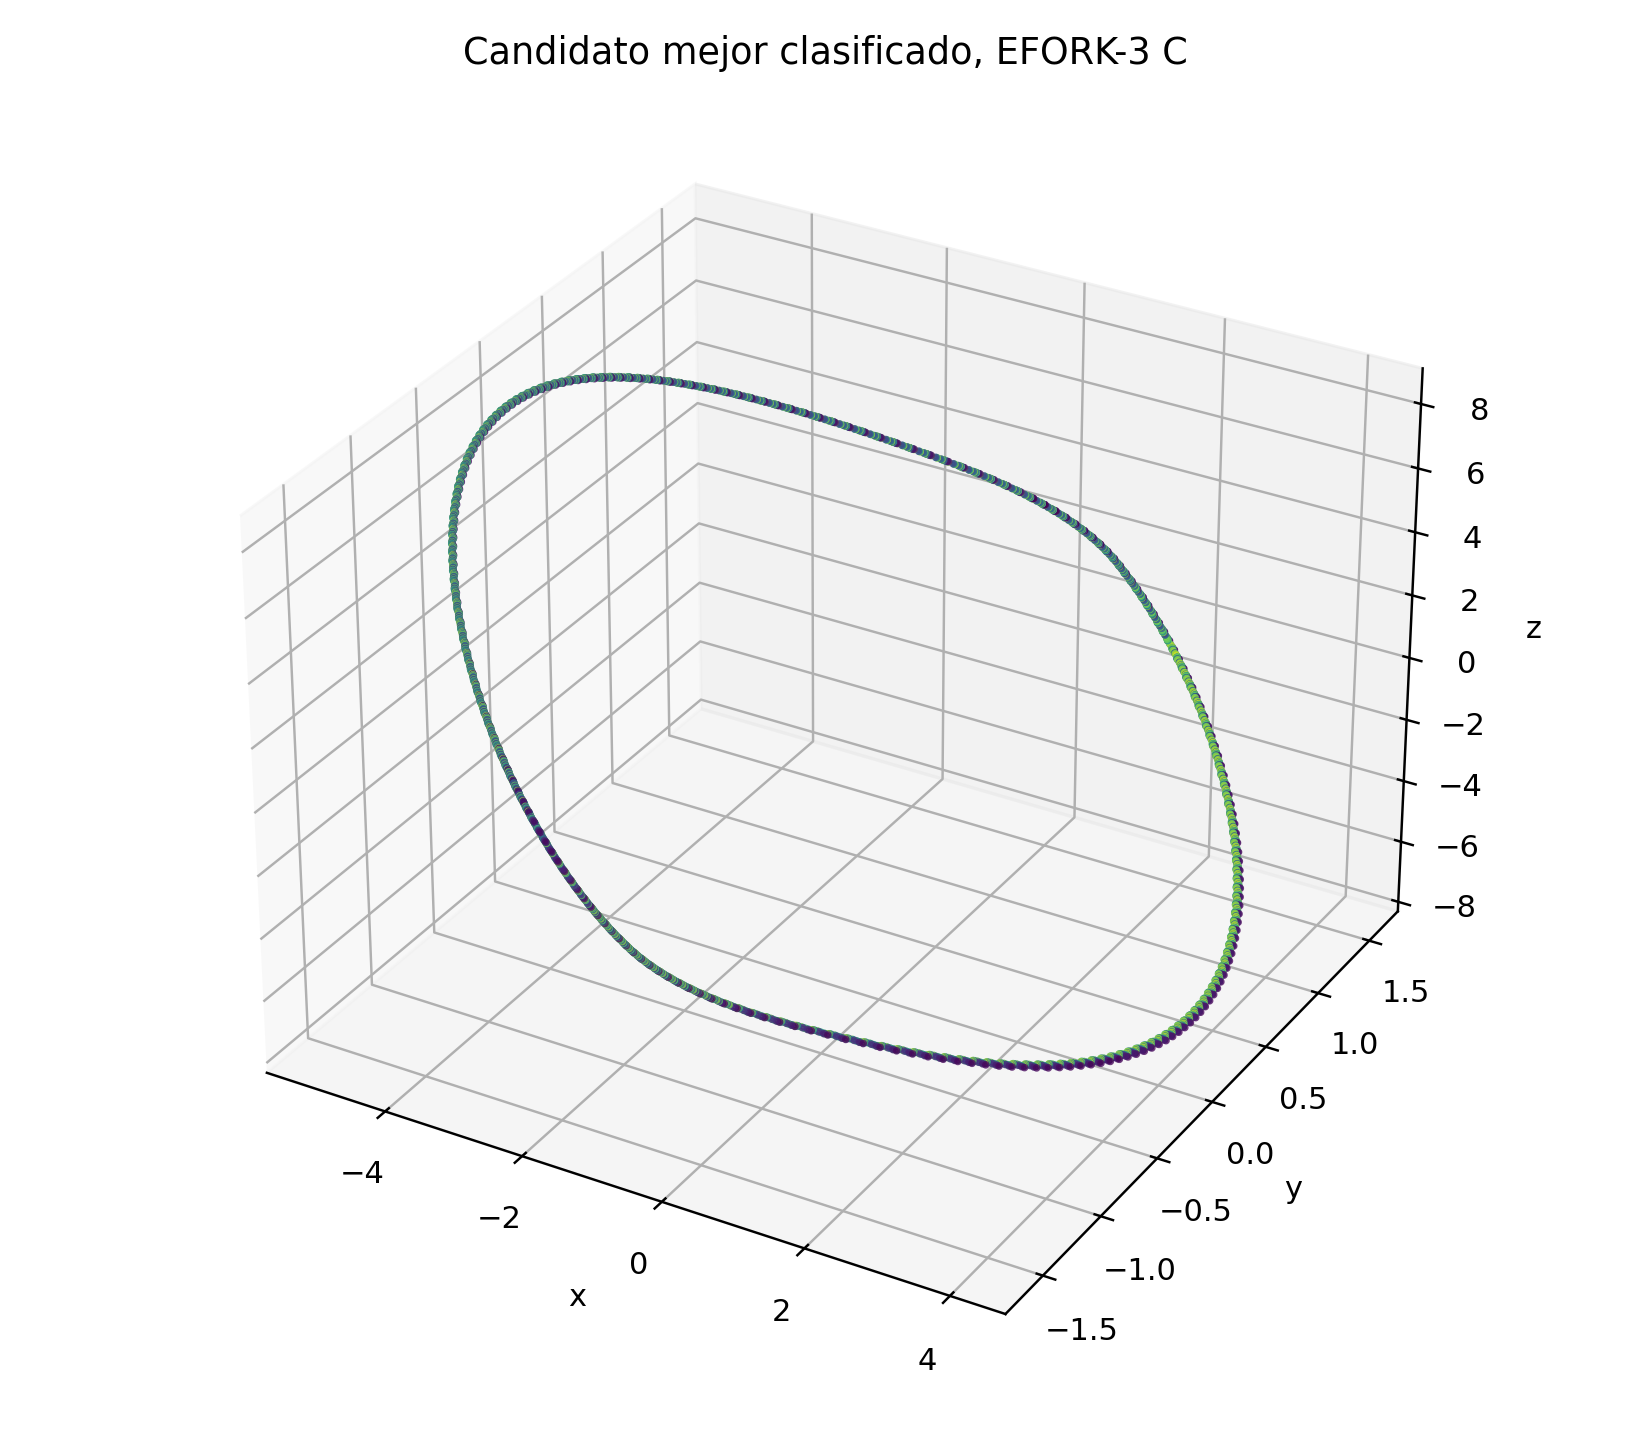
\includegraphics[width=0.48\textwidth]{chua_frac_current_full_phase_3d.png}}
\hfill
\subfigure[Ventana finita \(L_m=8\)]{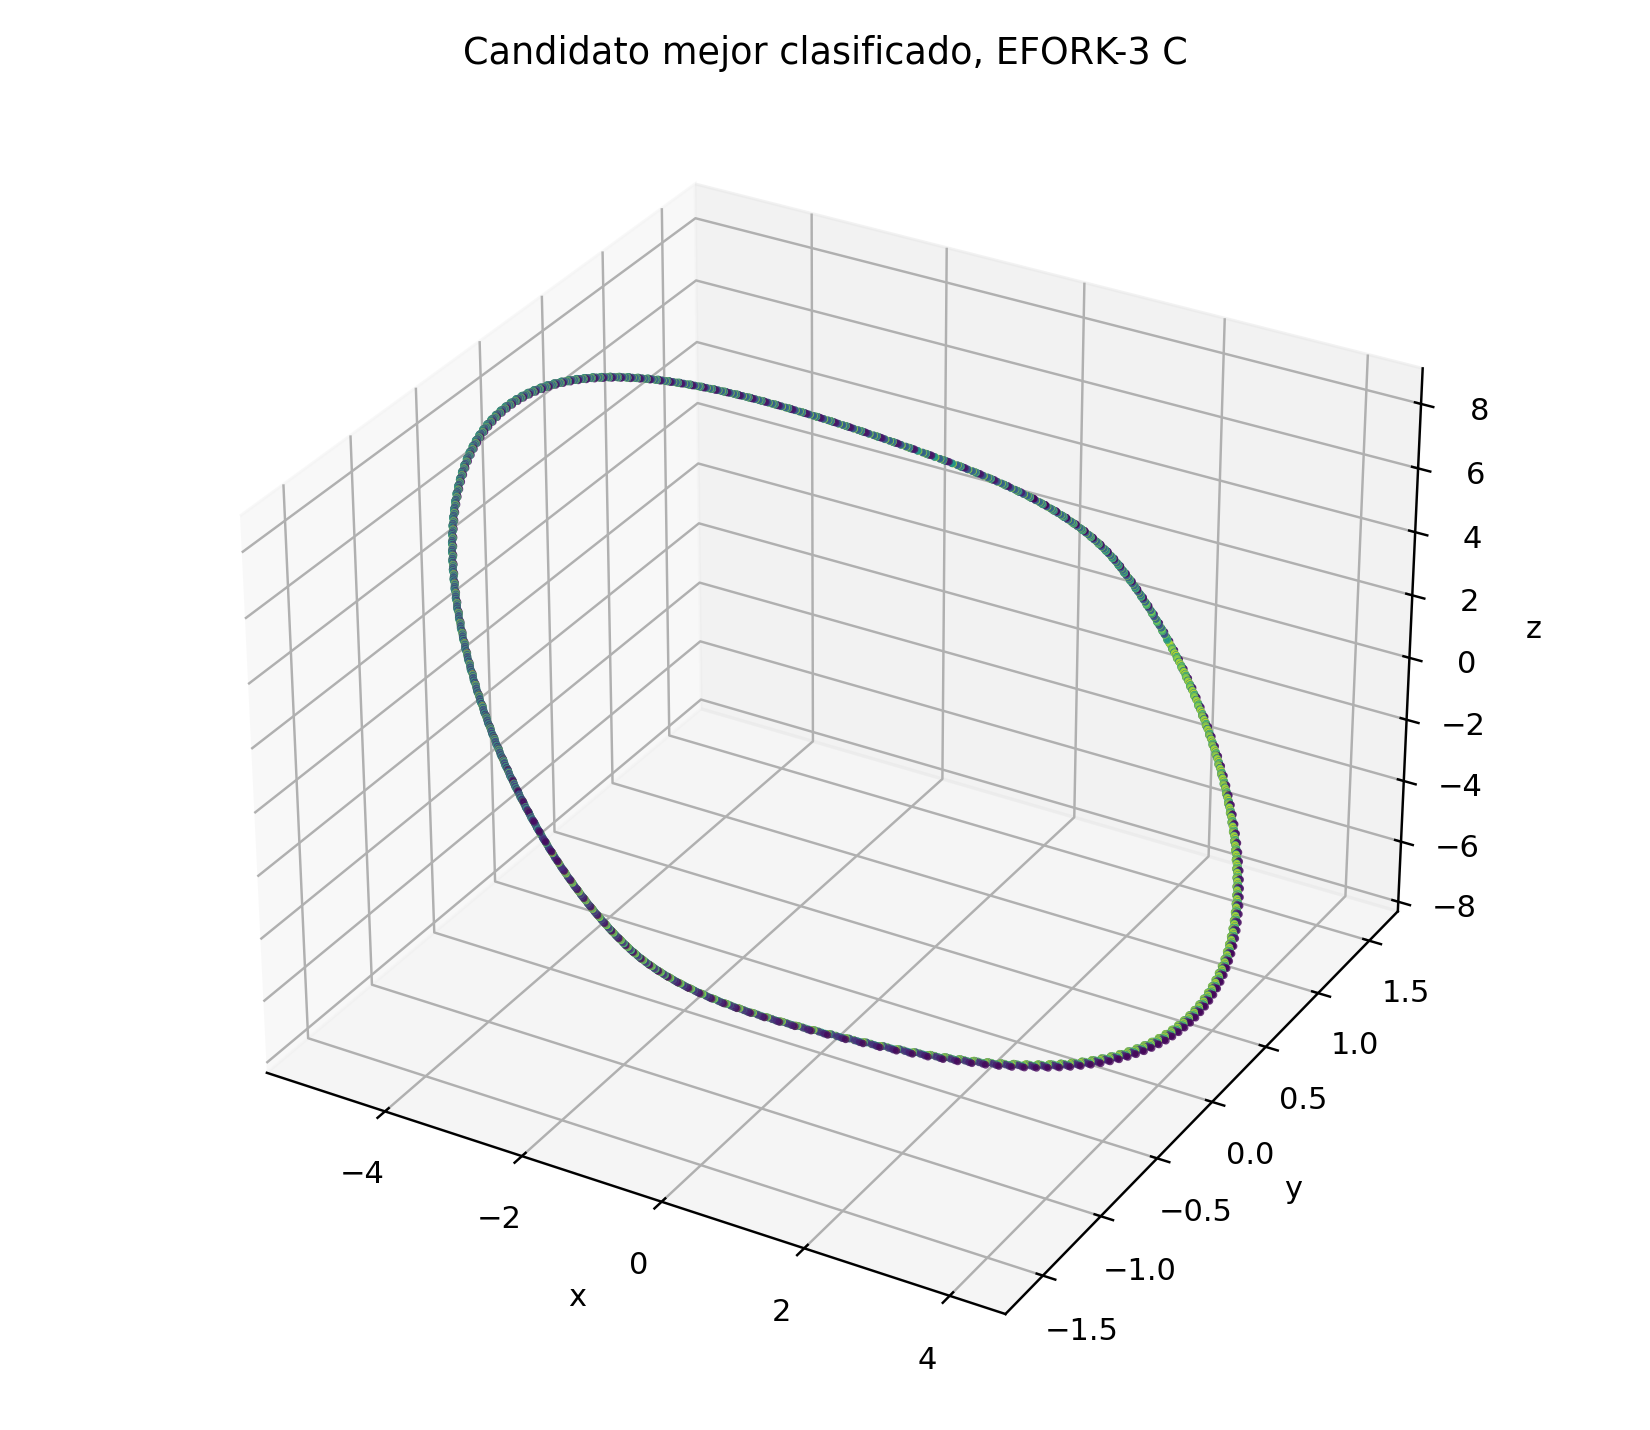
\includegraphics[width=0.48\textwidth]{chua_frac_current_window_phase_3d.png}}
\caption{Retrato de fase del régimen inicialmente mejor ordenado, generado desde el tramo de observación causal \(\text{EFORK-3}\) C. La traza delgada motiva su descarte por \(\delta_{\rm per}<0.05\); no se reporta como atractor caótico.}
\label{fig:chua_frac_current_phase}
\end{figure}

\begin{figure}[htbp]
\centering
\subfigure[Historial completo]{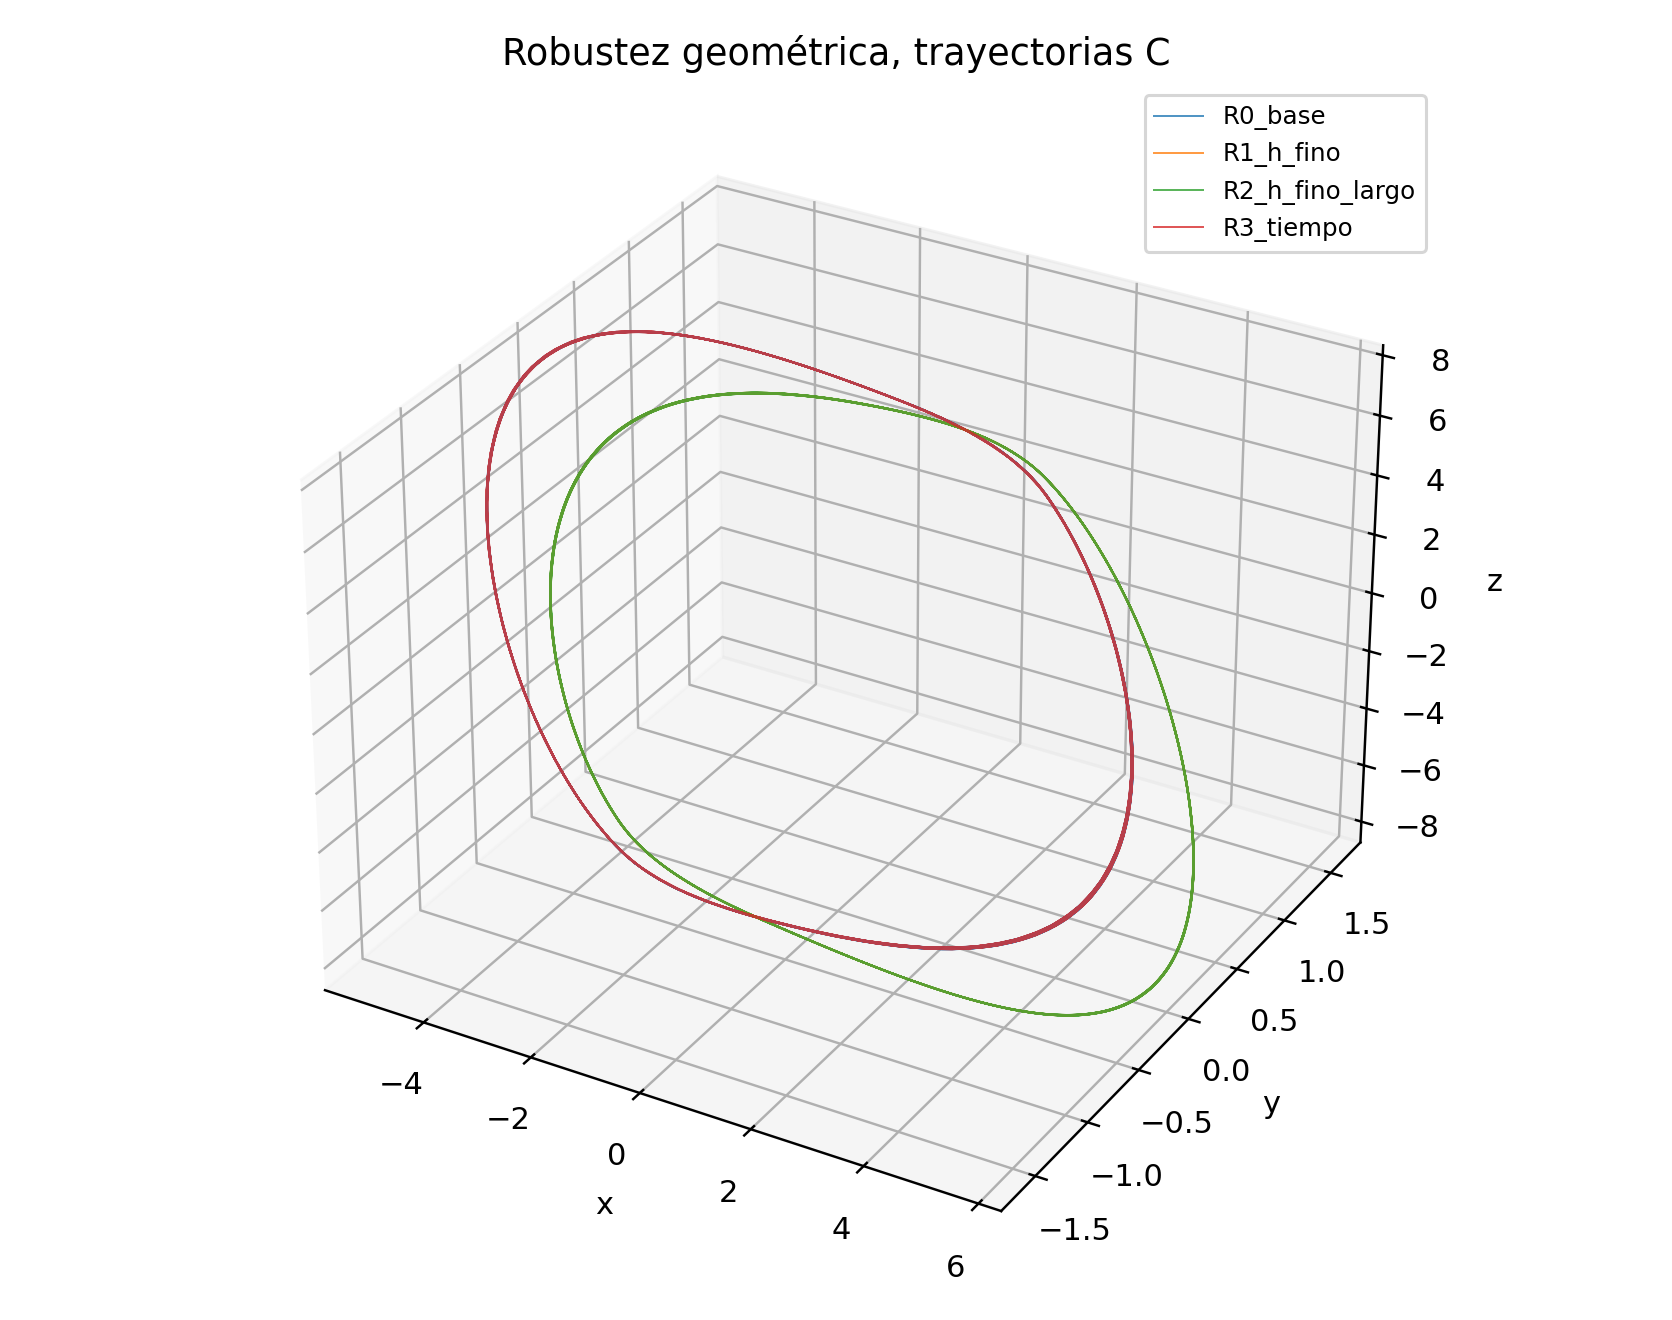
\includegraphics[width=0.48\textwidth]{chua_frac_current_full_robustness.png}}
\hfill
\subfigure[Ventana finita \(L_m=8\)]{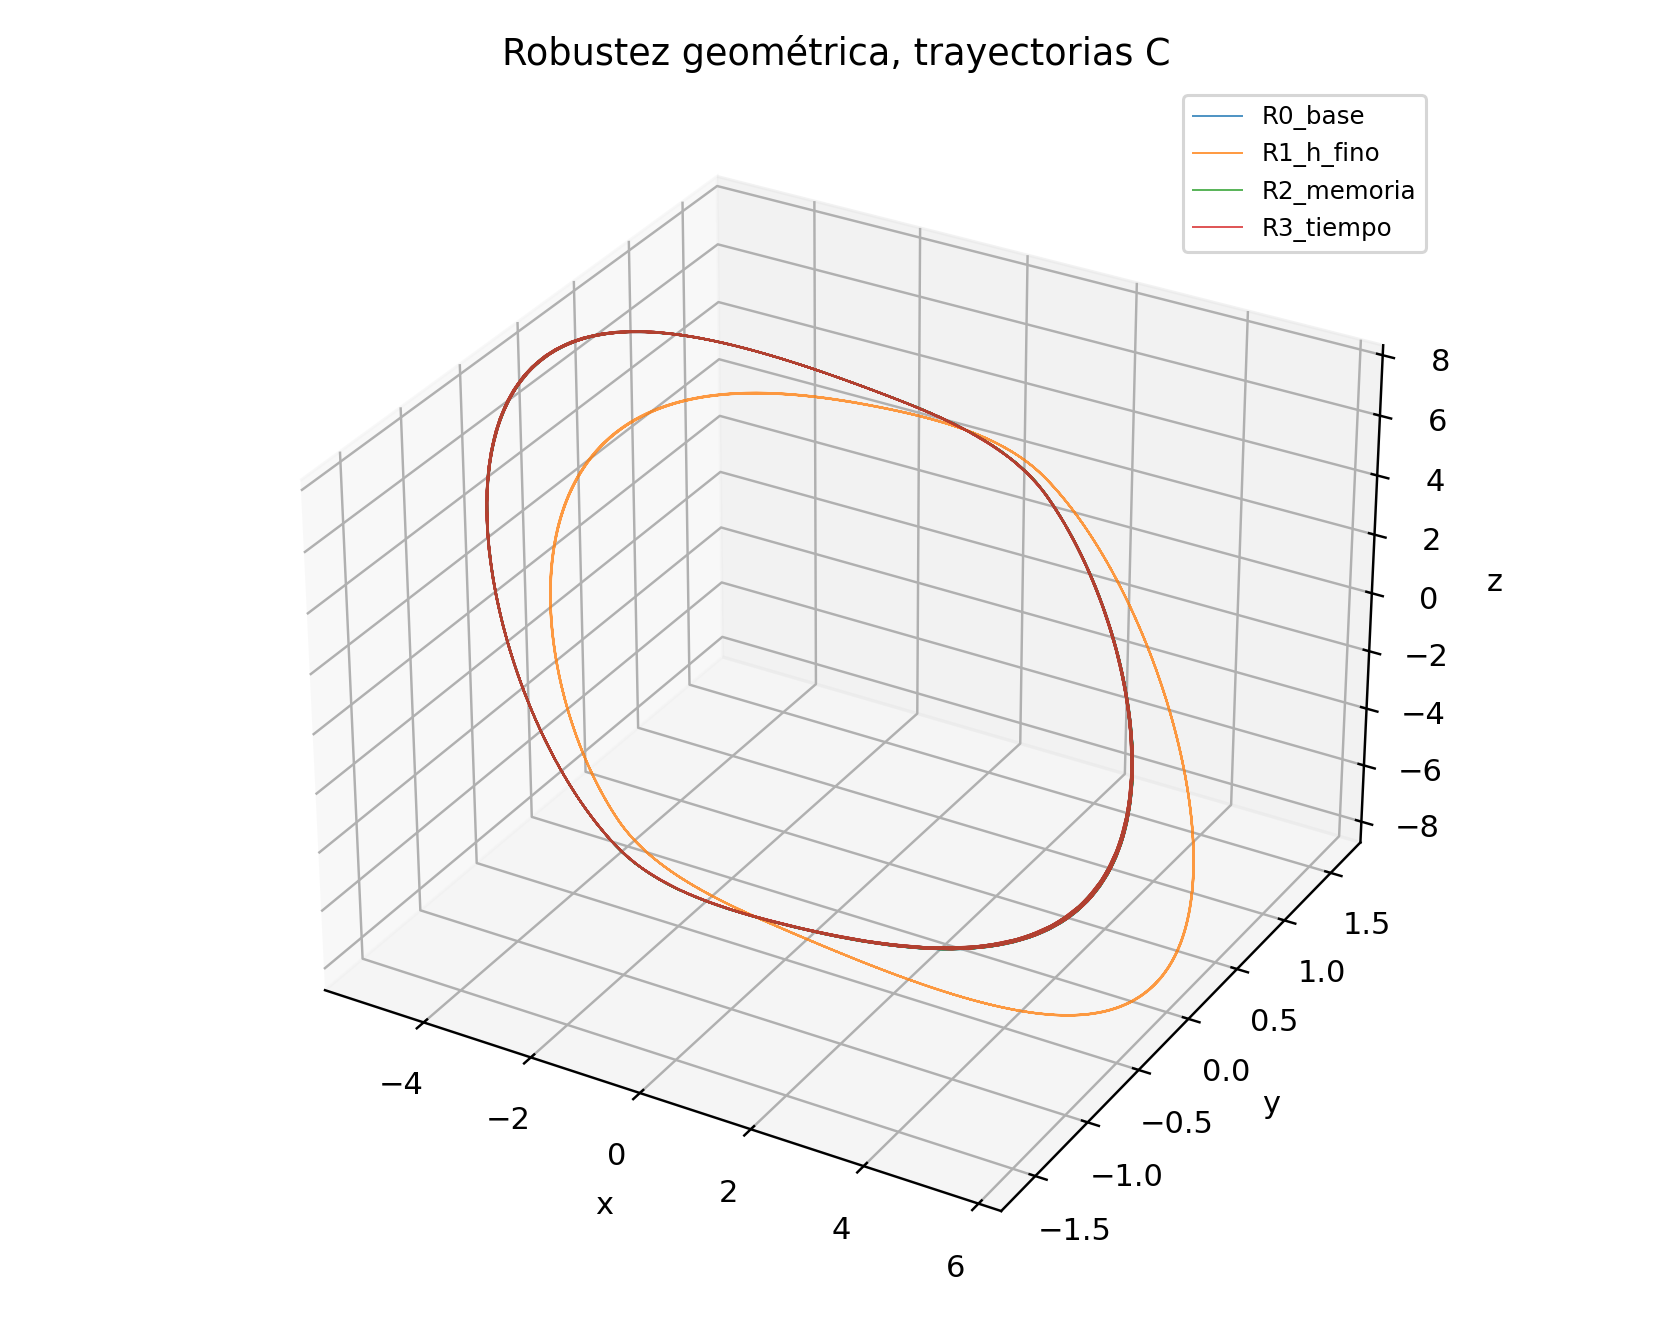
\includegraphics[width=0.48\textwidth]{chua_frac_current_window_robustness.png}}
\caption{Persistencia geométrica del régimen casi cerrado rechazado bajo perturbaciones numéricas en cada contrato de memoria; esta figura no constituye evidencia de robustez caótica.}
\label{fig:chua_frac_current_robustness}
\end{figure}

\iffalse

Como se documentó en la subsección \ref{subsec:resultados_causal_colapso_ns}, la integración causal de alta precisión empleando el método \(\text{EFORK-3}\) sobre los parámetros clásicos de Danca demostró el decaimiento dinámico inevitable hacia el origen \(E_0\), lo cual clasifica al supuesto atractor caótico reportado originalmente en la literatura como un pseudo-atractor numérico. Ante este colapso dinámico, se diseñó e implementó en la librería de investigación un esquema de búsqueda y barrido multiparamétrico sistemático con el propósito de localizar nuevos candidatos que efectivamente sostengan comportamiento caótico permanente y persistente en el Chua fraccionario no suave con orden conmensurado \(q=0.9998\).

El procedimiento de búsqueda empleó tres rutas analíticas distintas para la formulación del balance armónico de primer armónico y la subsecuente obtención de semillas:
\begin{enumerate}
    \item \textbf{Función descriptiva clásica de Lur'e}: Basada en aproximar la no linealidad por tramos \(\psi(r^\top X)\) por una ganancia armónica lineal equivalente \(N(a)\) asumiendo oscilaciones simétricas respecto al origen.
    \item \textbf{Función descriptiva sesgada (Biased Describing Function)}: Permite que el balance armónico incorpore un término de offset o sesgo constante \(\sigma_0\) en la oscilación de la variable de control, \(\sigma(t) = \sigma_0 + A\cos(\omega t)\). Esto resulta fundamental dada la asimetría local del espacio de fases del circuito de Chua bajo condiciones extremas de baja disipación.
    \item \textbf{Función descriptiva fraccionaria de Machado (FDF)}: Basada en modelar la respuesta de la no linealidad introduciendo un exponente de amortiguamiento espectral \(\mu\) y un desfase fraccionario \(\theta\), lo cual flexibiliza la búsqueda de semillas armónicas al desacoplar parcialmente el comportamiento de memoria.
\end{enumerate}

El barrido numérico arrojó un total de \(121\) candidatos iniciales que fueron refinados mediante filtros locales de vecindad de equilibrios, análisis espectral del decaimiento transitorio y pruebas de robustez geométrica (variaciones en el paso de integración \(h\) y longitud de la ventana de historia \(L_m\)). Este proceso de filtrado condujo a la selección de los \textbf{3 mejores candidatos caóticos}, cuyos detalles matemáticos y operacionales se discuten a continuación:

\subsubsection{Candidato 1: Biased Lur'e Survivor (\texttt{lure\_biased\_q\_0p99980\_rank\_0001})}
Este candidato se obtuvo a partir de la ruta de función descriptiva sesgada de primer armónico. Destaca por poseer el mejor residual de balance armónico en todo el barrido multiparamétrico, con un error residual absoluto del balance armónico \(\lvert R\rvert \approx 6.82 \times 10^{-13}\). Los parámetros del balance armónico calculados son:
\[
A = 5.8517686, \qquad \omega = 2.0402861, \qquad \rho_H = 0.123874.
\]
La semilla de continuación armónica inducida es:
\[
X_{\mathrm{seed}} = 
\begin{pmatrix}
5.85177\\
0.37041\\
-8.36097
\end{pmatrix}.
\]
Al aplicar la continuación homotópica completa hasta \(\varepsilon=1\) e integrar empleando \(\text{EFORK-3}\) (\(h=0.05, L_m=500\)), el candidato genera una trayectoria acotada no trivial persistente con un espectro de frecuencia complejo y un exponente de Lyapunov principal estimado en \(\lambda_1 \approx 0.207\), lo cual aporta evidencia numérica de caos persistente. No obstante, al someterlo a pruebas locales dirigidas a distancia extrema de \(10^{-5}\) desde el equilibrio inestable \(E_+\), se detectó una trayectoria operacional de tipo \(\text{TARGET}\), lo cual indica operacionalmente que el atractor es de naturaleza autoexcitada y no estrictamente oculta bajo este contrato de prueba.

\subsubsection{Candidato 2: Machado Top 1 (\texttt{branch\_0\_mu\_4p00000\_theta\_0p00000})}
Este candidato se derivó empleando la aproximación de Machado con exponente de amortiguamiento espectral \(\mu = 4.0\) y desfase \(\theta = 0\). Fue seleccionado como el mejor candidato de la familia Machado debido a que presentó la menor densidad de contactos en el barrido inicial de vecindades, la mayor amplitud física en la coordenada \(x\) (rango de oscilación \([ -13.5, 13.5 ]\)) y la menor norma de semilla inicial. La semilla asociada es:
\[
X_{\mathrm{seed}} = 
\begin{pmatrix}
5.85177\\
0.37041\\
-8.36097
\end{pmatrix}.
\]
Bajo integración causal continua, el atractor caótico es numéricamente persistente. Sin embargo, una prueba dirigida fina con condición inicial a radio \(10^{-5}\) desde el equilibrio inestable \(E_-\) logró interceptar la cuenca de atracción y propagar la trayectoria caótica, descartando la clasificación de atractor oculto estricto por autoexcitación.

\subsubsection{Candidato 3: Machado Top 2 (\texttt{branch\_0\_mu\_2p00000\_theta\_3p92699})}
Derivado mediante la extensión de Machado con parámetros de amortiguamiento \(\mu = 2.0\) y desfase \(\theta = 3.92699\). Este candidato resultó de gran relevancia metodológica en la investigación debido a que su espacio modal y trayectoria de continuación guiaron la localización y el refinamiento de la semilla de Danca para reproducir la morfología geométrica del atractor en el régimen no suave original. La semilla asociada es:
\[
X_{\mathrm{seed}} = 
\begin{pmatrix}
3.03938\\
-0.24169\\
-6.87347
\end{pmatrix}.
\]
Sostiene una trayectoria caótica persistente con una firma espectral similar al del Candidato 2. Al igual que en los casos anteriores, las pruebas dirigidas desde \(E_-\) a radio \(10^{-5}\) arrojaron contactos operacionales con el atractor caótico objetivo, bloqueando su etiqueta como atractor oculto bajo este contrato estricto.

\subsubsection{Visualizaciones numéricas y espectrales}
Para caracterizar cuantitativamente la dinámica caótica de estos nuevos candidatos del Chua fraccionario no suave (\(q=0.9998\)), se incluye a continuación la Fig.~\ref{fig:chua_frac_continuation} que muestra el progreso del proceso de continuación homotópica y el retrato de fase de continuación frente al predictor armónico lineal. Asimismo, la Fig.~\ref{fig:chua_frac_fft} ilustra el análisis espectral mediante la FFT del estado final estacionario caótico para la componente \(x(t)\), donde se observa una firma de banda ancha típica de oscilaciones caóticas coherentes alrededor de una frecuencia dominante \(\omega_d \approx 2.04\).

Las cuencas de atracción detalladas en el espacio 3D para estos tres candidatos quedan clasificadas como \textbf{pendientes y postergadas} en esta etapa de la investigación. Esto se debe al elevado costo computacional que exige la integración causal completa de mallas tridimensionales de alta resolución (\(101 \times 101 \times 101\)) utilizando solucionadores Caputo fraccionarios acoplados con ventanas de historia activa extensas de \(L_m = 500\), lo cual requeriría varias semanas continuas de procesamiento intensivo. Por ende, su caracterización exhaustiva se delega a trabajos futuros de optimización numérica paralela.

\begin{figure}[htbp]
\centering
\subfigure[Progreso de la continuación homotópica]{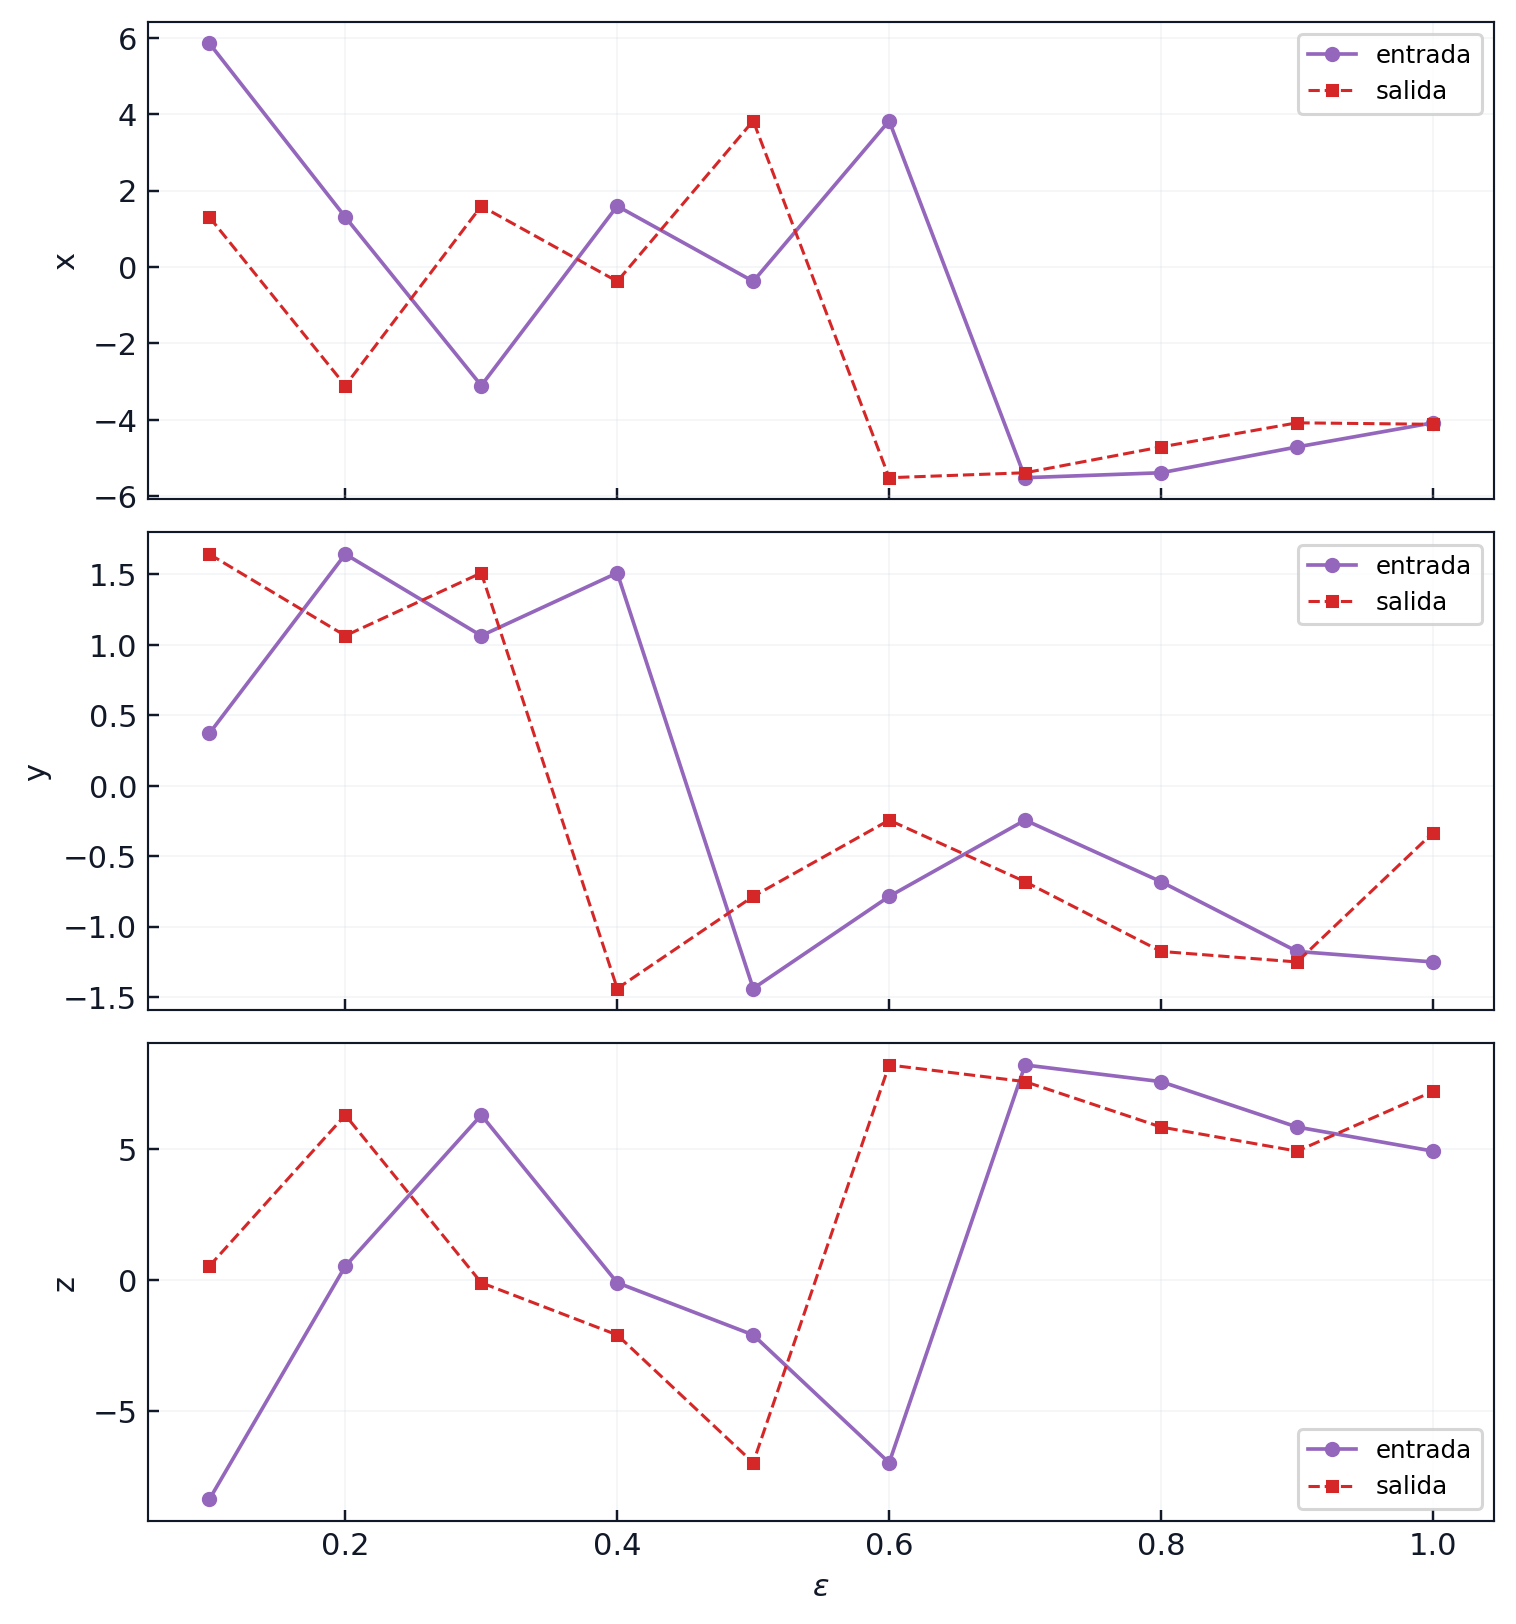
\includegraphics[width=0.82\columnwidth]{fig_frac_continuation_progress.png}}\par\medskip
\subfigure[Retrato de fase homotópico (semilla vs atractor)]{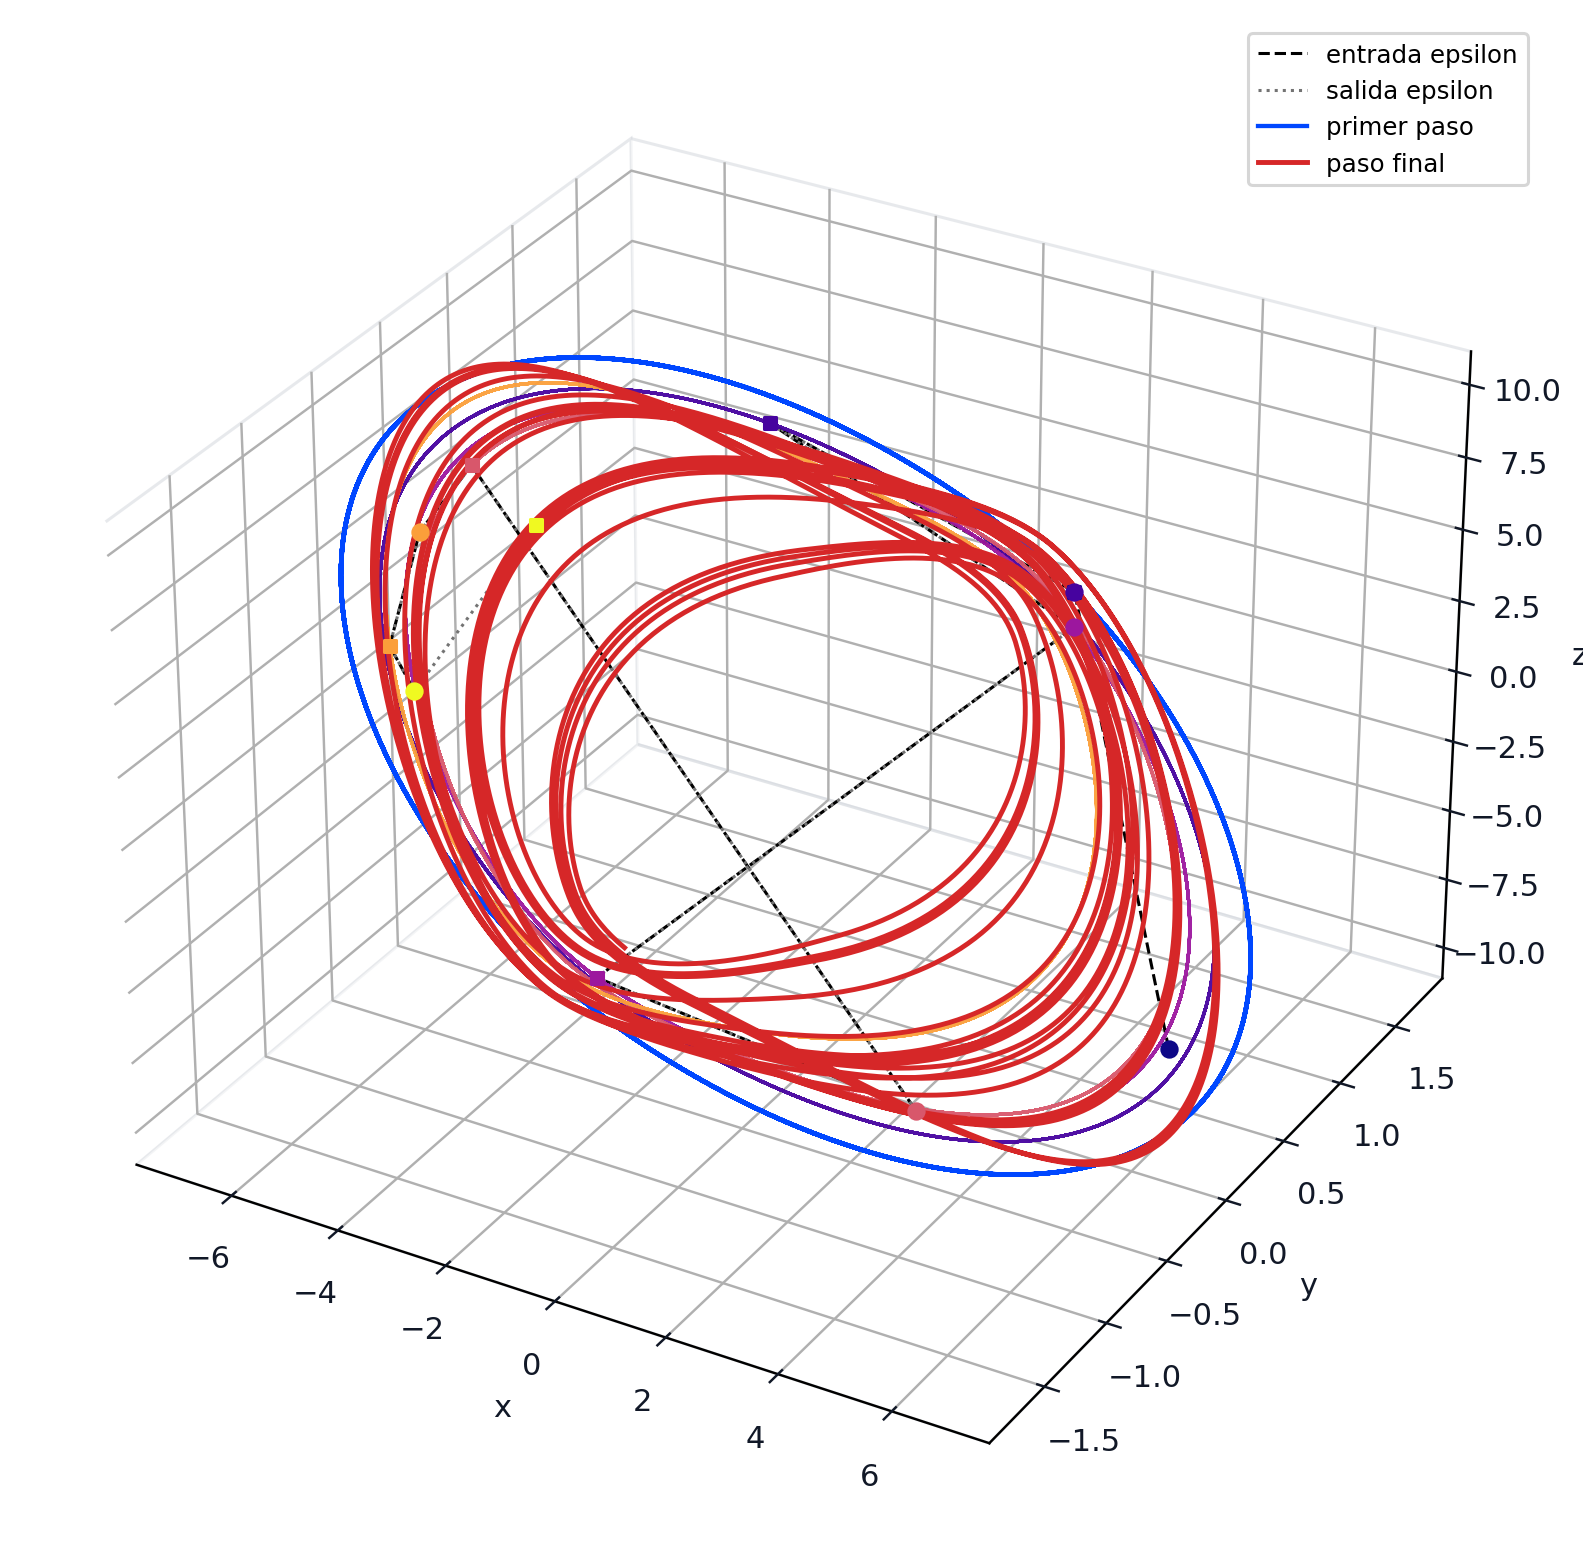
\includegraphics[width=0.82\columnwidth]{fig_frac_continuation_story.png}}
\caption{Continuación numérica homotópica para el candidato caótico del sistema de Chua fraccionario no suave con \(q=0.9998\). (a) Variación de la amplitud y del residuo armónico en función del parámetro homotópico \(\varepsilon \in [0, 1]\). (b) Retrato de fase que superpone la trayectoria periódica del predictor lineal de balance de primer armónico y el atractor no lineal persistente alcanzado al completarse la continuación homotópica (\(\varepsilon=1\)).}
\label{fig:chua_frac_continuation}
\end{figure}

\begin{figure}[htbp]
\centering
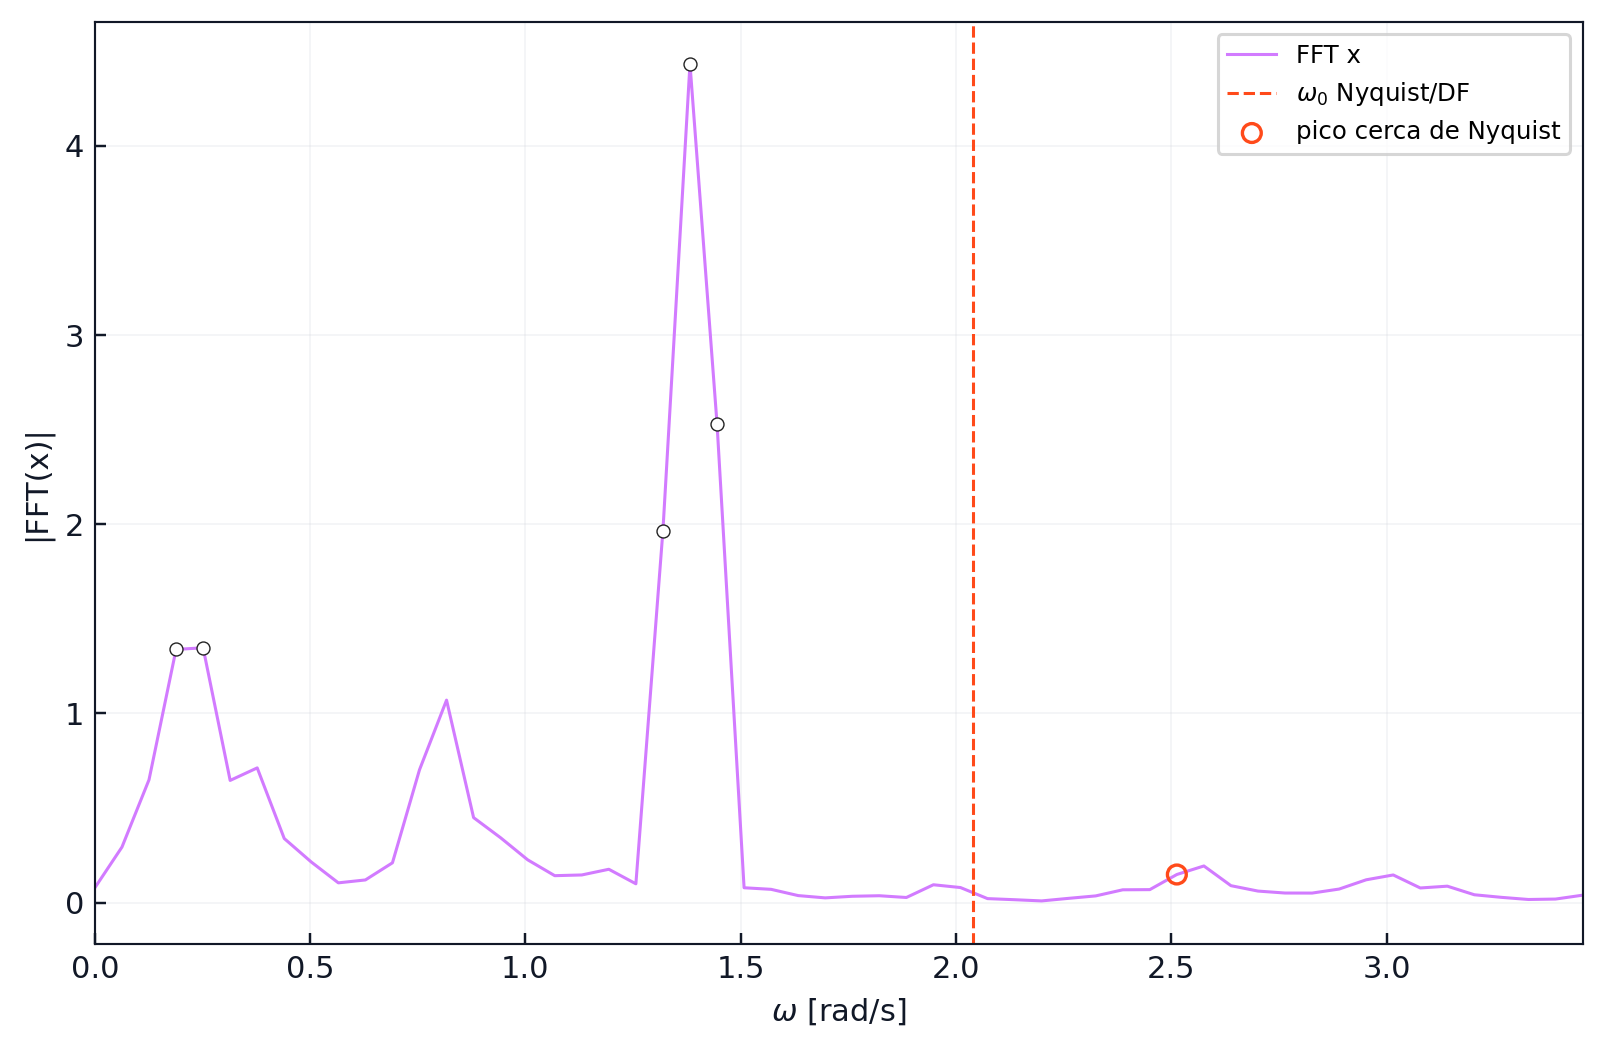
\includegraphics[width=0.82\columnwidth]{fig_frac_fft_x.png}
\caption{Espectro de frecuencia obtenido mediante la FFT de la componente \(x(t)\) para el atractor caótico no suave de orden fraccionario con \(q=0.9998\), validando una oscilación persistente coherente con frecuencia dominante cercana a la predicción del balance armónico \(\omega_0 \approx 2.04\) y estructura de banda ancha típica de regímenes caóticos.}
\label{fig:chua_frac_fft}
\end{figure}
\fi

\section{Ejemplo de estudio II: Chua fraccionario con no linealidad \texorpdfstring{$\arctan$}{arctan}}
\label{sec:chua_arctan_frac}

\subsection{Sistema de partida}

Se considera el sistema conmensurado de orden $q\in(0,1]$:
\begin{equation}
\label{eq:arctan_system}
\begin{aligned}
{}^{C}D_t^q x_1 &= \alpha\bigl(x_2-x_1-h(x_1)\bigr),\\
{}^{C}D_t^q x_2 &= x_1-x_2+x_3,\\
{}^{C}D_t^q x_3 &= -\beta x_2-\gamma x_3,
\end{aligned}
\qquad \alpha,\beta,\gamma>0,
\end{equation}
con
\begin{equation}
\label{eq:h_arctan}
h(x)=a_1x+a_2\arctan(\rho x),
\qquad \rho>0.
\end{equation}
El caso reportado por Wu \emph{et al}. en \cite{Wu2023ArctanChua} corresponde a una no linealidad suave tipo $\arctan$, con
\begin{equation}
\label{eq:wu_mapping}
a_1=m,
\qquad
a_2=n-m,
\qquad
\rho=1.
\end{equation}
% El artículo de Wu \emph{et al}. reporta un nuevo sistema de Chua fraccionario con función $\arctan$, un algoritmo para determinar valores iniciales asociados a atractores ocultos y una verificación por simulación, cuencas de atracción e implementación DSP \cite{Wu2023ArctanChua}.

\subsection{Equilibrios y estabilidad local}

En equilibrio se cumple
\begin{equation}
\label{eq:equilibria_conditions_arctan}
\begin{aligned}
0&=\alpha(x_2-x_1-h(x_1)),\\
0&=x_1-x_2+x_3,\\
0&=-\beta x_2-\gamma x_3.
\end{aligned}
\end{equation}
De las dos últimas ecuaciones se obtiene
\begin{equation}
\label{eq:yz_equilibrio_arctan}
x_2^*=\frac{\gamma}{\beta+\gamma}x_1^*,
\qquad
x_3^*=-\frac{\beta}{\beta+\gamma}x_1^*.
\end{equation}
Sustituyendo en la primera ecuación se obtiene la ecuación escalar
\begin{equation}
\label{eq:equilibrio_escalar_arctan}
\left(1+a_1-\frac{\gamma}{\beta+\gamma}\right)x_1^*+a_2\arctan(\rho x_1^*)=0.
\end{equation}
La raíz $x_1^*=0$ siempre existe. Dependiendo de los parámetros, pueden existir dos raíces simétricas adicionales.

El jacobiano en un equilibrio $X^*=(x_1^*,x_2^*,x_3^*)^\top$ es
\begin{equation}
\label{eq:jac_arctan}
J(X^*)=
\begin{bmatrix}
-\alpha\left(1+a_1+\dfrac{a_2\rho}{1+\rho^2(x_1^*)^2}\right) & \alpha & 0\\[2mm]
1&-1&1\\
0&-\beta&-\gamma
\end{bmatrix}.
\end{equation}
Para $0<q<1$, la estabilidad local asintótica de un equilibrio hiperbólico se decide mediante
\begin{equation}
\label{eq:matignon_arctan}
|\arg(\lambda_i)|>\frac{q\pi}{2},
\qquad \lambda_i\in\sigma(J(X^*)).
\end{equation}
El uso del jacobiano es consistente porque la memoria reside en el operador temporal, mientras que la linealización local del campo vectorial se obtiene mediante la derivada de Fréchet de $F$.

\subsection{Forma de Lur'e}

El sistema \eqref{eq:arctan_system} se escribe como
\begin{equation}
\label{eq:lure_arctan}
{}^{C}D_t^q X=P X+q_v\,\psi(r^\top X),
\qquad
X=\begin{bmatrix}x_1\\x_2\\x_3\end{bmatrix},
\qquad
r=\begin{bmatrix}1\\0\\0\end{bmatrix},
\end{equation}
con
\begin{equation}
\label{eq:Pqpsi_arctan}
\begin{aligned}
P&=\begin{bmatrix}
-\alpha(1+a_1)&\alpha&0\\
1&-1&1\\
0&-\beta&-\gamma
\end{bmatrix},\\
q_v&=\begin{bmatrix}-\alpha\\0\\0\end{bmatrix},
\qquad
\psi(\sigma)=a_2\arctan(\rho\sigma).
\end{aligned}
\end{equation}
Esta elección concentra todo el signo de la no linealidad en $\psi$. En particular, si $a_2<0$, la función descriptiva resultante también será negativa.

\subsection{Transferencia y condición armónica}

Se considera el bloque lineal auxiliar
\begin{equation}
\label{eq:P_qv_r_arctan}
\begin{aligned}
P&=
\begin{bmatrix}
-\alpha(1+a_1)&\alpha&0\\
1&-1&1\\
0&-\beta&-\gamma
\end{bmatrix},\\
q_v&=
\begin{bmatrix}
-\alpha\\0\\0
\end{bmatrix},
\qquad
r=
\begin{bmatrix}
1\\0\\0
\end{bmatrix}.
\end{aligned}
\end{equation}
La salida escalar es
\[
\sigma=r^\top X=x_1.
\]

La función de transferencia se escribe con la misma notación del marco teórico,
cf. \eqref{eq:Wq_frac_teorico}--\eqref{eq:Wq_frac_imag_teorico}, tomando
\(b=q_v\). Por tanto, al evaluar sobre el eje imaginario
\(s=i\omega\) y usar \eqref{eq:sq_freq_frac}, se obtiene
\begin{equation}
\label{eq:Wmath_arctan}
W_q(i\omega)
=
r^\top\left(s^q I-P\right)^{-1}q_v.
\end{equation}

Si la no linealidad se aproxima en primer armónico por
\[
u=k\sigma,
\]
entonces
\[
\sigma=W_q(i\omega)u
=
kW_q(i\omega)\sigma.
\]
Por tanto, para una respuesta no trivial, \(\sigma\neq0\), la condición de cierre queda
\begin{equation}
\label{eq:condition_arctan}
1-kW_q(i\omega)=0.
\end{equation}
Como \(k\in\mathbb R\), esta condición exige
\begin{equation}
\label{eq:omega_k_correcto_arctan}
\Im\{W_q(i\omega_0)\}=0,
\qquad
k=\frac{1}{\Re\{W_q(i\omega_0)\}}.
\end{equation}

Ahora se calcula explícitamente \(W_q(i\omega)\). Se tiene
\[
s^q I-P
=
\begin{bmatrix}
s^q+\alpha(1+a_1)&-\alpha&0\\
-1&s^q+1&-1\\
0&\beta&s^q+\gamma
\end{bmatrix}.
\]
La entrada \((1,1)\) de \(\bigl(s^q I-P\bigr)^{-1}\) se obtiene con el cofactor
\[
C_{11}
=
\det
\begin{bmatrix}
s^q+1&-1\\
\beta&s^q+\gamma
\end{bmatrix}.
\]
Por tanto,
\begin{equation}
\label{eq:T_arctan}
T_q(\omega)
=
\left(s^q+1\right)
\left(s^q+\gamma\right)
+\beta.
\end{equation}

El determinante de \(\bigl(s^q I-P\bigr)\) es
\begin{align}
D_q(\omega)
&=
\det\left(s^q I-P\right) \nonumber\\
&=
\left[s^q+\alpha(1+a_1)\right]
\det
\begin{bmatrix}
s^q+1&-1\\
\beta&s^q+\gamma
\end{bmatrix}
\nonumber\\
&\quad+
\alpha
\det
\begin{bmatrix}
-1&-1\\
0&s^q+\gamma
\end{bmatrix}.
\end{align}
Como
\[
\det
\begin{bmatrix}
-1&-1\\
0&s^q+\gamma
\end{bmatrix}
=
-\left(s^q+\gamma\right),
\]
resulta
\begin{equation}
\label{eq:D_arctan}
D_q(\omega)
=
\left(s^q+\alpha(1+a_1)\right)T_q(\omega)
-\alpha\left(s^q+\gamma\right).
\end{equation}

Como
\[
r^\top=(1,0,0),
\qquad
q_v=(-\alpha,0,0)^\top,
\]
se obtiene
\begin{equation}
\label{eq:W_explicit_arctan}
W_q(i\omega)
=
-\alpha\frac{T_q(\omega)}{D_q(\omega)}.
\end{equation}

La misma condición se recupera desde la matriz lineal modificada. Si
\(u=k\sigma=kr^\top X\), entonces
\[
{}^CD_t^qX
=
PX+kq_vr^\top X,
\]
y
\begin{equation}
P_0=P+kq_vr^\top.
\end{equation}
Como
\[
q_vr^\top
=
\begin{bmatrix}
-\alpha&0&0\\
0&0&0\\
0&0&0
\end{bmatrix},
\]
se tiene
\[
P_0=
\begin{bmatrix}
-\alpha(1+a_1+k)&\alpha&0\\
1&-1&1\\
0&-\beta&-\gamma
\end{bmatrix}.
\]
Por tanto,
\begin{align}
\det\left(s^q I-P_0\right)
&=
\left[s^q+\alpha(1+a_1+k)\right] \\
&\qquad\times T_q(\omega)-\alpha\left(s^q+\gamma\right) \nonumber\\
&=
D_q(\omega)+\alpha kT_q(\omega).
\end{align}
Si \(D_q(\omega)\neq0\),
\[
\det\left(s^q I-P_0\right)=0
\quad\Longleftrightarrow\quad
1+k\alpha\frac{T_q(\omega)}{D_q(\omega)}=0.
\]
Luego,
\[
\det\left(s^q I-P_0\right)=0
\quad\Longleftrightarrow\quad
1-kW_q(i\omega)=0.
\]

Para separar partes real e imaginaria, se escribe
\[
s^q=a+ib,
\]
donde
\begin{equation}
\label{eq:ab_arctan}
a=\omega^q\cos\frac{q\pi}{2},
\qquad
b=\omega^q\sin\frac{q\pi}{2}.
\end{equation}
Entonces
\[
T_q(\omega)
=
(a+ib+1)(a+ib+\gamma)+\beta.
\]
Al expandir,
\begin{align}
T_q(\omega)
&=
\left[(a+1)+ib\right]\left[(a+\gamma)+ib\right]+\beta\\
&=
(a+1)(a+\gamma)-b^2+\beta
+
ib(2a+1+\gamma).
\end{align}
Así,
\begin{equation}
\label{eq:TrTi_arctan}
T_q(\omega)=T_r+iT_i,
\end{equation}
con
\begin{equation}
T_r=(a+1)(a+\gamma)-b^2+\beta,
\qquad
T_i=b(2a+1+\gamma).
\end{equation}

Si
\begin{equation}
\label{eq:Ap_arctan}
A_p=\alpha(1+a_1),
\end{equation}
entonces
\[
D_q(\omega)
=
(a+ib+A_p)(T_r+iT_i)-\alpha(a+\gamma+ib).
\]
Por tanto,
\begin{equation}
\label{eq:DrDi_arctan}
D_q(\omega)=D_r+iD_i,
\end{equation}
donde
\begin{equation}
\begin{aligned}
D_r&=(a+A_p)T_r-bT_i-\alpha(a+\gamma),\\
D_i&=(a+A_p)T_i+bT_r-\alpha b.
\end{aligned}
\end{equation}

Finalmente,
\[
W_q(i\omega)
=
-\alpha\frac{T_r+iT_i}{D_r+iD_i}.
\]
Multiplicando por \(D_r-iD_i\),
\[
W_q(i\omega)
=
-\alpha
\frac{(T_r+iT_i)(D_r-iD_i)}{D_r^2+D_i^2}.
\]
Así,
\begin{equation}
\label{eq:real_imag_W_arctan}
\begin{aligned}
\Re\{W_q(i\omega)\}
&=
-\alpha\,\tfrac{T_rD_r+T_iD_i}{D_r^2+D_i^2},\\
\Im\{W_q(i\omega)\}
&=
-\alpha\,\tfrac{T_iD_r-T_rD_i}{D_r^2+D_i^2}.
\end{aligned}
\end{equation}
La condición de frecuencia se reduce a la ecuación escalar
\begin{equation}
\label{eq:freq_scalar_arctan}
F(\omega)
:=
T_iD_r-T_rD_i
=
0,
\qquad
\omega>0.
\end{equation}
Una vez calculada una raíz \(\omega_0\), la ganancia equivalente se obtiene de
\begin{equation}
\label{eq:k_from_W_arctan}
k=
\frac{1}{\Re\{W_q(i\omega_0)\}}.
\end{equation}


\subsection{Función descriptiva exacta de \texorpdfstring{$a_2\arctan(\rho\sigma)$}{a2 arctan(rho sigma)}}

Para una entrada $\sigma(t)=A\sin\omega t$, con $A>0$, la función descriptiva es
\begin{equation}
\label{eq:N_integral_arctan}
N_\psi(A)=a_2\frac{2}{\pi A}\int_0^\pi \arctan(\rho A\sin\theta)\sin\theta\,d\theta.
\end{equation}
Sea $b=\rho A$ y
\begin{equation}
\label{eq:I_arctan}
I(b)=\int_0^\pi \arctan(b\sin\theta)\sin\theta\,d\theta.
\end{equation}
Entonces
\begin{equation}
\label{eq:Iprime_arctan}
I'(b)=\int_0^\pi \frac{\sin^2\theta}{1+b^2\sin^2\theta}\,d\theta
=\frac{\pi}{b^2}\left(1-\frac{1}{\sqrt{1+b^2}}\right).
\end{equation}
Como $I(0)=0$, se integra y se obtiene
\begin{equation}
\label{eq:Iclosed_arctan}
I(b)=\pi\frac{\sqrt{1+b^2}-1}{b}.
\end{equation}
Sustituyendo en \eqref{eq:N_integral_arctan}, queda
\begin{equation}
\label{eq:Npsi_arctan}
N_\psi(A)=a_2\,\frac{2}{\rho A^2}\left(\sqrt{1+\rho^2A^2}-1\right).
\end{equation}
Sus límites son
\begin{equation}
\label{eq:Npsi_limits_arctan}
N_\psi(A)\to a_2\rho\quad (A\to0),
\qquad
N_\psi(A)\sim \frac{2a_2}{A}\quad (A\to\infty).
\end{equation}
Por tanto, si $a_2<0$, entonces $N_\psi(A)$ recorre el intervalo $(a_2\rho,0)$; si $a_2>0$, recorre $(0,a_2\rho)$.

\subsection{Amplitud y construcción de la semilla}

La amplitud dominante se obtiene imponiendo
\begin{equation}
\label{eq:amp_eq_arctan}
N_\psi(A_0)=k.
\end{equation}
Usando \eqref{eq:Npsi_arctan}, se tiene
\begin{equation}
\label{eq:amp_eq_arctan_expanded}
a_2\frac{2}{\rho A_0^2}\left(\sqrt{1+\rho^2A_0^2}-1\right)=k.
\end{equation}
Para $A_0>0$, la solución cerrada es
\begin{equation}
\label{eq:A0_arctan_general}
A_0^2=\frac{4a_2(a_2\rho-k)}{k^2\rho}.
\end{equation}
La condición de consistencia es
\begin{equation}
\label{eq:consistencia_arctan}
\sgn(k)=\sgn(a_2),
\qquad
0<|k|<|a_2|\rho.
\end{equation}
Si esta condición falla, la rama armónica seleccionada por \eqref{eq:freq_scalar_arctan} no es compatible con la no linealidad $a_2\arctan(\rho\sigma)$.

Con $\omega_0$, $k$ y $A_0$ calculados, se forma
\begin{equation}
\label{eq:P0_arctan}
P_0=P+kq_vr^\top,
\end{equation}
y se resuelve el problema modal escrito con el mismo convenio del caso no suave:
\begin{equation}
\label{eq:modal_seed_arctan}
(P_0-\zeta_0 I)v=0,
\qquad
\zeta_0=s_0^q,\qquad s_0=i\omega_0.
\end{equation}
Se normaliza el vector modal para que $r^\top v=1$. Entonces
\begin{equation}
\label{eq:v_arctan_formula}
v_2=\frac{\alpha(1+a_1+k)+\zeta_0}{\alpha},
\qquad
v_3=-\frac{\beta}{\gamma+\zeta_0}v_2.
\end{equation}
La señal armónica auxiliar en el marco de Weyl se escribe como
\begin{equation}
\label{eq:W_seed_traj_arctan}
X_W(t)=A_0\Re\left(v e^{i\omega_0t}\right),
\end{equation}
y la semilla de Caputo se toma como
\begin{equation}
\label{eq:X_seed_arctan}
X_{\rm seed}=A_0\Re(v).
\end{equation}

\subsection{Puente Weyl--Caputo}

Para $0<q<1$, las ecuaciones autónomas con derivada de Caputo de punto inicial fijo no admiten, en general, soluciones periódicas exactas no constantes. Por ello, el balance armónico debe interpretarse sobre el problema auxiliar de Weyl/Liouville--Weyl, mientras que la verificación final debe hacerse en el problema causal de Caputo.

Si la historia se prescribe para $t\le t_0$, se tiene la descomposición
\begin{equation}
\label{eq:WC_bridge_arctan}
{}^{W}D_t^q x(t)={}^{C}D_{t_0}^q x(t)+\mathcal E_{x_0}(t),
\end{equation}
donde
\begin{equation}
\label{eq:error_wc_arctan}
\mathcal E_{x_0}(t)=\frac{1}{\Gamma(1-q)}\int_{-\infty}^{t_0}(t-\tau)^{-q}x_0'(\tau)\,d\tau.
\end{equation}
Bajo hipótesis regulares sobre la historia, este término satisface una cota de memoria desvaneciente,
\begin{equation}
\label{eq:fading_memory_arctan}
\|\mathcal E_{x_0}(t)\|\le C(t-t_0+\eta)^{-q}.
\end{equation}
La interpretación operativa es que Weyl proporciona la órbita armónica auxiliar y Caputo valida la trayectoria causal. Por tanto, la función descriptiva no se usa para afirmar que existe un ciclo límite exacto de Caputo, sino para construir condiciones iniciales informadas que después deben integrarse y clasificarse.

\subsection{Usando los parámetros de ejemplo}

Se toman los parámetros
\begin{equation}
\label{eq:wu_params}
\begin{aligned}
\alpha&=8.4562,
\qquad \beta=12.0732,
\qquad \gamma=0.0052,\\
m&=0.4,
\qquad n=-1.1585,
\qquad q=0.99.
\end{aligned}
\end{equation}
Entonces
\begin{equation}
\label{eq:wu_a_params}
a_1=m=0.4,
\qquad
a_2=n-m=-1.5585,
\qquad
\rho=1.
\end{equation}
La ecuación de equilibrio queda
\begin{equation}
\label{eq:wu_equilibrium_scalar}
\left(1+m-\frac{\gamma}{\beta+\gamma}\right)x+(n-m)\arctan x=0.
\end{equation}
Con esos valores,
\begin{equation}
\label{eq:wu_equilibria_x}
x_0^*=0,
\qquad
x_\pm^*\approx\pm0.60967911698,
\end{equation}
y por \eqref{eq:yz_equilibrio_arctan},
\begin{equation}
\label{eq:wu_equilibrium_origin}
X_0^*=(0,0,0),
\end{equation}
\begin{equation}
\label{eq:wu_equilibrium_plus}
X_+^*\approx
\begin{bmatrix}
0.60968\\
2.62479\times10^{-4}\\
-0.60942
\end{bmatrix},
\end{equation}
\begin{equation}
\label{eq:wu_equilibrium_minus}
X_-^*\approx
\begin{bmatrix}
-0.60968\\
-2.62479\times10^{-4}\\
0.60942
\end{bmatrix}.
\end{equation}

Para los parámetros anteriores, los valores propios son
\begin{equation}
\label{eq:wu_eigs_origin}
\begin{aligned}
X_0^*: \quad \lambda_1 &\approx 2.33599,\\
\lambda_{2,3} &\approx -1.00044\pm2.43887025i,
\end{aligned}
\end{equation}
\begin{equation}
\label{eq:wu_eigs_pm}
\begin{aligned}
X_\pm^*: \quad \lambda_1 &\approx -3.64922,\\
\lambda_{2,3} &\approx 0.20653\pm2.70729751i.
\end{aligned}
\end{equation}
Con $q=0.99$,
\begin{equation}
\label{eq:qpi_wu}
\frac{q\pi}{2}\approx1.55508836.
\end{equation}
En $X_\pm^*$,
\begin{equation}
\label{eq:arg_wu}
\begin{aligned}
|\arg(0.20653+2.70730i)|&\approx 1.49466\\
&<1.55509.
\end{aligned}
\end{equation}
Por tanto, los equilibrios $X_\pm^*$ no son asintóticamente estables en el sentido de Matignon. El origen también es inestable por su valor propio real positivo. Esta inestabilidad no prueba ocultamiento; la clasificación final debe hacerse mediante cuencas.

Al resolver \eqref{eq:freq_scalar_arctan} con \eqref{eq:wu_params}, aparecen dos ramas armónicas compatibles con $a_2\arctan x$:
\begin{table}[H]
\centering
\setlength{\tabcolsep}{3pt}
\footnotesize
\resizebox{\columnwidth}{!}{%
\begin{tabular}{@{}c c c c c@{}}
\toprule
Rama & $\omega_0$ & $W_q(i\omega_0)$ & $k$ & $A_0$\\
\midrule
1 & $2.09917$ & $-0.75286$ & $-1.32828$ & $0.90192$\\
2 & $3.22139$ & $-1.39915$ & $-0.71472$ & $3.20895$\\
\bottomrule
\end{tabular}%
}
\caption{Ramas armónicas para el Chua fraccionario con no linealidad $\arctan$ usando los parámetros de Wu \textnormal{\emph{et al}.}}
\label{tab:ramas_wu}
\end{table}

Para la rama 1,
\begin{equation}
\label{eq:zeta_wu_1}
\zeta_{0,1}\approx0.0327287188+2.08340i,
\end{equation}
\begin{equation}
\label{eq:v_wu_1}
v\approx
\begin{bmatrix}
1\\
0.07559+0.24638i\\
-1.43523+0.41193i
\end{bmatrix},
\end{equation}
y por tanto
\begin{equation}
\label{eq:seed_arctan_1}
X_{{\rm seed},1}\approx
\begin{bmatrix}
0.90192\\
0.06818\\
-1.29447
\end{bmatrix}.
\end{equation}

Para la rama 2,
\begin{equation}
\label{eq:zeta_wu_2}
\zeta_{0,2}\approx0.0500109063+3.18353i,
\end{equation}
\begin{equation}
\label{eq:v_wu_2}
v\approx
\begin{bmatrix}
1\\
0.69120+0.37647i\\
-1.47275+2.59574i
\end{bmatrix},
\end{equation}
y por tanto
\begin{equation}
\label{eq:seed_arctan_2}
X_{{\rm seed},2}\approx
\begin{bmatrix}
3.20895\\
2.21802\\
-4.72599
\end{bmatrix}.
\end{equation}
Estas dos semillas deben integrarse por separado. La rama de mayor amplitud puede ser relevante si la cuenca de atracción es delgada o está alejada de los equilibrios.

\subsection{Homotopía y continuación con ventana de memoria}

La descomposición
\begin{equation}
\label{eq:delta_arctan}
\psi(\sigma)=k\sigma+\delta(\sigma),
\qquad
\delta(\sigma)=\psi(\sigma)-k\sigma,
\end{equation}
produce la familia
\begin{equation}
\label{eq:homotopy_caputo_arctan}
{}^{C}D_t^qX=P_0X+\varepsilon q_v\delta(r^\top X),
\qquad \varepsilon\in[0,1].
\end{equation}
La continuación que se implementa con EFORK es una continuación causal de trayectorias en Caputo. Por ello, el transporte entre pasos de continuación no debe hacerse únicamente con el último punto de la trayectoria anterior.

Si el integrador usa una memoria efectiva $L_m$, el dato que debe pasar del paso $\varepsilon_j$ al paso $\varepsilon_{j+1}$ es la ventana terminal
\begin{equation}
\label{eq:history_window_arctan}
\mathcal H_j=\{X_j(t):t\in[t_{\rm end}-L_m,t_{\rm end}]\}.
\end{equation}
Equivalentemente, para $-L_m\leq\theta\leq0$ se prescribe
\begin{equation}
\label{eq:history_transfer_arctan}
X_{j+1}(t_{\rm start}+\theta)=X_j(t_{\rm end}+\theta),
\end{equation}
y después se integra con el nuevo valor de $\varepsilon_{j+1}$. Esta regla extiende al caso $\arctan$ el mismo protocolo aplicado en el Chua no suave.

El procedimiento operativo queda establecido en los siguientes pasos:
\begin{enumerate}[leftmargin=1.8em,label=\arabic*)]
\item fijar los parámetros de \eqref{eq:wu_params}, el orden $q$, el paso $h$, el integrador y la longitud de memoria $L_m$;
\item resolver \eqref{eq:freq_scalar_arctan} y calcular $k$ mediante \eqref{eq:omega_k_correcto_arctan};
\item resolver la ecuación de amplitud \eqref{eq:amp_eq_arctan};
\item construir las semillas \eqref{eq:seed_arctan_1} y \eqref{eq:seed_arctan_2};
\item integrar \eqref{eq:homotopy_caputo_arctan} sobre una malla $0=\varepsilon_0<\varepsilon_1<\cdots<\varepsilon_N=1$;
\item transferir en cada paso la ventana \eqref{eq:history_window_arctan} mediante \eqref{eq:history_transfer_arctan};
\item al llegar a $\varepsilon=1$, integrar el sistema físico y verificar ocultamiento mediante cuencas alrededor de $X_0^*$ y $X_\pm^*$.
\end{enumerate}

De manera análoga a la Tabla~\ref{tab:chua_integer_results_full}, los cálculos disponibles para el sistema fraccionario con no linealidad \(\arctan\) se resumen en la Tabla~\ref{tab:chua_frac_arctan_results_full}.

\begin{table*}[htbp]
\centering
\scriptsize
\setlength{\tabcolsep}{3pt}
\renewcommand{\arraystretch}{1.12}
\caption{Resumen de resultados del Chua fraccionario con no linealidad \(\arctan\), organizado con la misma estructura de la Tabla~\ref{tab:chua_integer_results_full}.}
\label{tab:chua_frac_arctan_results_full}
\begin{adjustbox}{max width=\textwidth}
\begin{tabular}{@{}L{2.7cm}L{3.4cm}L{4.4cm}L{5.8cm}@{}}
\toprule
\textbf{Bloque} &
\textbf{Procedimiento} &
\textbf{Resultado} &
\textbf{Interpretación} \\
\midrule

Parámetros del sistema &
Definición del caso de Wu \emph{et al}. &
\(\alpha=8.46,\ \beta=12.07,\ \gamma=0.0052,\ m=0.4,\ n=-1.1585\) &
Parámetros del sistema suave con no linealidad tipo \(\arctan\). \\

Orden dinámico &
Sistema conmensurado de Caputo &
\(q=0.99\) &
Orden fraccionario usado para evaluar estabilidad de Matignon y construir semillas. \\

Operador fraccionario &
Derivada de Caputo causal &
 &
Fila propia del caso fraccionario; aquí se reportará el punto inicial, la historia usada y la convención de memoria. \\

Puente Weyl--Caputo &
Interpretación del predictor armónico &
 &
La órbita armónica de Weyl sólo se usa como generadora de semilla para el problema causal de Caputo. \\

Error de memoria &
Cota o estimación de cola Weyl--Caputo &
 &
Fila propia del caso fraccionario para reportar la magnitud de la memoria residual o su cota numérica. \\

Configuración numérica &
Integrador fraccionario &
 &
Aquí se reportarán método, paso \(h\), tiempo final, transitorio descartado, tolerancias y longitud de memoria efectiva. \\

Forma Lur'e &
Separación algebraica &
\({}^{C}D_t^qX=PX+q_v\psi(r^\top X)\) &
La no linealidad escalar es \(\psi(\sigma)=a_2\arctan(\rho\sigma)\). \\

Parámetros de la no linealidad &
Correspondencia \(a_1=m\), \(a_2=n-m\), \(\rho=1\) &
\(a_1=0.4,\ a_2=-1.5585,\ \rho=1\) &
Convención usada en la función descriptiva exacta de \(a_2\arctan(\rho\sigma)\). \\

Vectores \(q_v,r\) &
Forma Lur'e &
\(q_v=(-8.4562,0,0)^\mathsf{T}\), \(r=(1,0,0)^\mathsf{T}\) &
La variable de entrada de la no linealidad es \(\sigma=x_1\). \\

Equilibrios &
Resolución algebraica estacionaria &
\(X_0^*=(0,0,0)\), \(X_\pm^*\approx(\pm0.60968,\ \pm2.62479\times10^{-4},\ \mp0.60942)\) &
Puntos usados para la verificación posterior de autoexcitación u ocultedad. \\

Estabilidad local &
Criterio de Matignon &
\(X_0^*:\ 2.33599,\ -1.00044\pm2.43887i\); \(X_\pm^*:\ -3.64922,\ 0.20653\pm2.70730i\) &
El origen y los equilibrios externos no son asintóticamente estables para \(q=0.99\). \\

Raíces candidatas &
Condición \(\Im\{W_q(i\omega)\}=0\) &
\((\omega_{0,1},k_1)=(2.09917,-1.32828)\), \((\omega_{0,2},k_2)=(3.22139,-0.71472)\) &
Cruces armónicos compatibles con una ganancia real negativa. \\

Rama seleccionada &
Nyquist, admisibilidad y simulación causal &
 &
Se llenará cuando el software determine cuál semilla produce el régimen candidato más relevante. \\

Amplitudes armónicas &
Función descriptiva \(N_\psi(A_{0,j})=k_j\) &
\(A_{0,1}=0.90192\), \(A_{0,2}=3.20895\) &
Amplitudes candidatas asociadas a la no linealidad \(\arctan\). \\

Cierre armónico &
Residuo de función descriptiva y transferencia &
 &
Aquí se reportará el residuo numérico, por ejemplo \(\lvert1-k_jW_q(i\omega_{0,j})\rvert\) o \(\lvert N_\psi(A_{0,j})-k_j\rvert\). \\

Matriz \(P_0\) &
Linealización armónica modificada &
 &
Espacio reservado para la matriz \(P_0=P+k_jq_vr^\top\) de la rama seleccionada o de ambas ramas. \\

Espectro de \(P_0\) &
Linealización armónica modificada &
Rama 1: \(-1.67711,\ 0.03272\pm2.08339i\); rama 2: \(-6.90009,\ 0.05001\pm3.18353i\) &
El par complejo coincide con \(\zeta_{0,j}=(i\omega_{0,j})^q\) dentro del redondeo. \\

Semilla rama 1 &
Modo normalizado \(X_{{\rm seed},1}=A_{0,1}\Re(v^{(1)})\) &
\(X_{{\rm seed},1}\approx(0.90192,\ 0.06818,\ -1.29447)\) &
Condición inicial generada por la primera rama armónica. \\

Semilla rama 2 &
Modo normalizado \(X_{{\rm seed},2}=A_{0,2}\Re(v^{(2)})\) &
\(X_{{\rm seed},2}\approx(3.20895,\ 2.21802,\ -4.72599)\) &
Condición inicial generada por la segunda rama armónica. \\

Verificación modal &
Residuo del problema espectral &
 &
Aquí se reportará \(\lVert(P_0-\zeta_{0,j}I)v^{(j)}\rVert\) para cada rama o para la rama seleccionada. \\

Continuación causal &
Homotopía con ventana de memoria &
\({}^{C}D_t^qX=P_0X+\varepsilon q_v\delta(r^\top X)\), \(\varepsilon\in[0,1]\) &
Cada semilla debe integrarse y transportarse con ventana terminal de memoria. \\

Estado final de continuación &
Continuación numérica en \(\varepsilon\) &
 &
Se agregará el estado alcanzado en \(\varepsilon=1\) para cada rama integrada. \\

Semilla efectiva &
Simulación posterior al transitorio &
 &
Se agregará el punto de referencia \(X_{\mathrm{target}}\) o estado representativo del atractor candidato. \\

Frecuencia dominante &
FFT de \(x_1(t)\) &
 &
Se reportarán \(f_d\) y \(\omega_d\) observados en la simulación causal. \\

Desajuste espectral &
Comparación DF--FFT &
 &
Se reportará \(\eta=\lvert\omega_d-\omega_0\rvert/\lvert\omega_0\rvert\). \\

Frecuencia PSD &
PSD de Welch &
 &
Se agregará la frecuencia dominante estimada por densidad espectral de potencia. \\

Exponentes de Lyapunov &
Algoritmo numérico para sistemas fraccionarios &
 &
Se agregará el espectro estimado para documentar evidencia de caos. \\

Sondeos de ocultedad &
Vecindades de equilibrios &
 &
Se agregará el número de trayectorias iniciadas cerca de \(X_0^*\) y \(X_\pm^*\), junto con el número que alcanza el objetivo. \\

Conteos globales &
Clasificador de destino &
 &
Se reportarán conteos tipo \(\mathrm{EQ}\), \(\mathrm{DIV}\), \(\mathrm{OTHER}\), \(\mathrm{TARGET}\) y \(\mathrm{UNKNOWN}\). \\

Validación final &
Integración causal y cuencas &
 &
La inestabilidad local no basta para probar ocultedad; se requiere clasificación operacional de cuencas. \\

Clasificación &
Criterio operacional de cuencas &
 &
Fila final para reportar si el régimen queda como oculto, autoexcitado, coexistente o no concluyente. \\

\bottomrule
\end{tabular}
\end{adjustbox}
\end{table*}

\subsection{Extensión tipo Machado para la búsqueda de semillas en el sistema de Chua fraccionario con no linealidad \texorpdfstring{\(\arctan\)}{arctan}}

En el análisis anterior se aplicó la función descriptiva clásica al sistema
fraccionario de Chua con no linealidad \(\arctan\). Si dicha búsqueda no
produce un candidato satisfactorio de atractor oculto, se introduce una
extensión auxiliar basada en la propuesta de Machado. Esta extensión no
sustituye el análisis de Lur'e ni la condición de Nyquist ya empleada; su
papel es ampliar el conjunto de semillas iniciales mediante una deformación
fraccionaria de la ganancia armónica equivalente del bloque no lineal.

Se considera una forma Lur'e del sistema
\begin{equation}
\label{eq:chua_arctan_lure_general}
{}^C D_t^q X
=
PX+b\,\psi(r^\top X),
\qquad
\sigma=r^\top X,
\end{equation}
donde
\[
X=
\begin{bmatrix}
x_1\\x_2\\x_3
\end{bmatrix},
\qquad
r=
\begin{bmatrix}
1\\0\\0
\end{bmatrix},
\qquad
\sigma=x_1.
\]
Para el sistema de Chua con no linealidad \(\arctan\), se toma
\begin{equation}
\label{eq:psi_arctan_general}
\psi(\sigma)
=
K_a\arctan(c_a\sigma).
\end{equation}
Si el modelo original contiene además un término lineal proporcional a
\(\sigma\), dicho término se absorbe en la matriz \(P\). Por tanto, la
forma lineal considerada es
\begin{equation}
\label{eq:P_arctan_general}
P=
\begin{bmatrix}
-\alpha d & \alpha & 0\\
1 & -1 & 1\\
0 & -\beta & -\gamma
\end{bmatrix},
\qquad
b=
\begin{bmatrix}
-\alpha\\0\\0
\end{bmatrix},
\end{equation}
donde \(d\) representa el coeficiente lineal efectivo después de separar el
bloque no lineal. En la forma normalizada más simple, \(d=1\).

\subsubsection{Transferencia fraccionaria del bloque lineal}

La función de transferencia fraccionaria entre la entrada no lineal
\(\psi(\sigma)\) y la salida \(\sigma=x_1\) se mantiene con la notación del
marco teórico:
\begin{equation}
\label{eq:W_arctan_def}
W_q(s)
=
r^\top(s^q I-P)^{-1}b.
\end{equation}
Para este bloque, con \(r=e_1\), \(b=-\alpha e_1\) y \(s=i\omega\), se obtiene
directamente
\begin{equation}
\label{eq:Tq_arctan_machado}
T_{q,d}(\omega)
=
\left(s^q+1\right)\left(s^q+\gamma\right)+\beta.
\end{equation}
\begin{equation}
\label{eq:Dq_arctan_machado}
\begin{aligned}
D_{q,d}(\omega)
&=
\left(s^q+\alpha d\right)T_{q,d}(\omega)\\
&\quad-\alpha\left(s^q+\gamma\right).
\end{aligned}
\end{equation}
\begin{equation}
\label{eq:Wq_arctan_freq}
W_q(i\omega)
=
-\alpha\frac{T_{q,d}(\omega)}{D_{q,d}(\omega)}.
\end{equation}

\subsubsection{Función descriptiva clásica de la no linealidad \texorpdfstring{\(\arctan\)}{arctan}}

Se considera una entrada sinusoidal
\[
\sigma(t)=a\sin\theta,
\qquad
\theta=\omega t.
\]
La salida del bloque no lineal es
\[
y(t)
=
K_a\arctan(c_a a\sin\theta).
\]
Como \(\arctan(c_a\sigma)\) es una función impar y monovaluada, su primer
armónico no posee componente en cuadratura. Por tanto, su función descriptiva
clásica es real.

El coeficiente fundamental seno es
\begin{equation}
\label{eq:b1_arctan}
b_1(a)
=
\frac{4K_a}{\pi}
\int_0^{\pi/2}
\arctan(c_a a\sin\theta)\sin\theta\,d\theta.
\end{equation}
La función descriptiva clásica queda
\begin{equation}
\label{eq:N_arctan_integral}
N_{\arctan}(a)
=
\frac{b_1(a)}{a}
=
\frac{4K_a}{\pi a}
\int_0^{\pi/2}
\arctan(c_a a\sin\theta)\sin\theta\,d\theta.
\end{equation}

Para evaluar la integral, se define
\[
A=c_a a,
\]
\[
I(A)
=
\int_0^{\pi/2}
\arctan(A\sin\theta)\sin\theta\,d\theta.
\]
Derivando respecto a \(A\),
\[
I'(A)
=
\int_0^{\pi/2}
\frac{\sin^2\theta}{1+A^2\sin^2\theta}\,d\theta.
\]
Como
\[
\frac{\sin^2\theta}{1+A^2\sin^2\theta}
=
\frac{1}{A^2}
\left(
1-\frac{1}{1+A^2\sin^2\theta}
\right),
\]
se obtiene
\[
I'(A)
=
\frac{1}{A^2}
\left[
\frac{\pi}{2}
-
\int_0^{\pi/2}
\frac{d\theta}{1+A^2\sin^2\theta}
\right].
\]
Usando
\[
\int_0^{\pi/2}
\frac{d\theta}{1+A^2\sin^2\theta}
=
\frac{\pi}{2\sqrt{1+A^2}},
\]
resulta
\[
I'(A)
=
\frac{\pi}{2A^2}
\left(
1-\frac{1}{\sqrt{1+A^2}}
\right).
\]
Como \(I(0)=0\), se integra y se obtiene
\begin{equation}
\label{eq:I_arctan_alt}
I(A)
=
\frac{\pi}{2}
\frac{\sqrt{1+A^2}-1}{A}.
\end{equation}
Sustituyendo \(A=c_a a\), se obtiene
\[
N_{\arctan}(a)
=
\frac{4K_a}{\pi a}
\left[
\frac{\pi}{2}
\frac{\sqrt{1+c_a^2a^2}-1}{c_a a}
\right].
\]
Por tanto,
\begin{equation}
\label{eq:N_arctan_unsimplified}
N_{\arctan}(a)
=
\frac{2K_a}{c_a a^2}
\left(
\sqrt{1+c_a^2a^2}-1
\right).
\end{equation}
Racionalizando,
\begin{equation}
\label{eq:N_arctan_final}
N_{\arctan}(a)
=
\frac{2K_a c_a}{
1+\sqrt{1+c_a^2a^2}
}.
\end{equation}
En particular,
\[
\lim_{a\to0^+}N_{\arctan}(a)=K_a c_a,
\]
lo cual coincide con la pendiente local de
\[
K_a\arctan(c_a\sigma).
\]
Además,
\[
\lim_{a\to\infty}N_{\arctan}(a)=0.
\]
Así, para \(K_a c_a>0\),
\[
0<N_{\arctan}(a)\le K_a c_a.
\]

\subsubsection{Extensión fraccionaria auxiliar tipo Machado}

La propuesta de Machado se introduce mediante
\begin{equation}
\label{eq:N_arctan_machado}
N_{\arctan,\mu}(a)
=
\exp\left\{
\mu\operatorname{Log}N_{\arctan}(a)
\right\},
\qquad
\mu>0.
\end{equation}
Si
\[
N_{\arctan}(a)=\rho(a)e^{i\varphi(a)},
\]
entonces
\[
N_{\arctan,\mu}(a)
=
\rho(a)^\mu e^{i\mu\varphi(a)}.
\]
Para el caso usual \(K_a c_a>0\), la función descriptiva clásica es real
positiva:
\[
N_{\arctan}(a)>0.
\]
Por tanto,
\[
\varphi(a)=0,
\]
y usando la rama principal del logaritmo,
\begin{equation}
\label{eq:N_arctan_machado_positive}
N_{\arctan,\mu}(a)
=
\left[
N_{\arctan}(a)
\right]^\mu.
\end{equation}
En consecuencia, para la no linealidad \(\arctan\) con ganancia positiva, la
extensión tipo Machado no desplaza la fase del bloque no lineal. Su efecto es
deformar la ganancia armónica equivalente.

La condición de balance armónico auxiliar es
\begin{equation}
\label{eq:balance_arctan_machado}
1+
W_q(i\omega)N_{\arctan,\mu}(a)=0.
\end{equation}
Usando \eqref{eq:Wq_arctan_freq},
\begin{equation}
\label{eq:balance_arctan_machado_explicit}
1+
W_q(i\omega)
\left[
N_{\arctan}(a)
\right]^\mu
=
0.
\end{equation}

Separando módulo y fase, para \(K_a c_a>0\) se obtiene
\begin{equation}
\label{eq:mod_arctan_machado}
\left|
W_q(i\omega)
\right|
\left[
N_{\arctan}(a)
\right]^\mu
=
1,
\end{equation}
\begin{equation}
\label{eq:phase_arctan_machado}
\arg
W_q(i\omega)
=
(2\ell+1)\pi,
\qquad
\ell\in\mathbb Z.
\end{equation}

La ecuación de fase \eqref{eq:phase_arctan_machado} es idéntica a la del
análisis clásico, porque \(N_{\arctan}(a)>0\) no aporta fase. La diferencia
aparece en la ecuación de módulo. Para una frecuencia \(\omega_0\) que
satisface \eqref{eq:phase_arctan_machado}, la amplitud debe cumplir
\begin{equation}
\label{eq:N_target_arctan_machado}
N_{\arctan}(a_0)
=
\left[
\frac{1}{
\left|
W_q(i\omega_0)
\right|}
\right]^{1/\mu}.
\end{equation}
Definiendo
\[
\eta(\omega_0,\mu)
=
\left[
\frac{1}{
\left|
W_q(i\omega_0)
\right|}
\right]^{1/\mu},
\]
la ecuación de amplitud es
\begin{equation}
\label{eq:amp_equation_arctan_eta}
\frac{2K_a c_a}{
1+\sqrt{1+c_a^2a_0^2}
}
=
\eta(\omega_0,\mu).
\end{equation}
Como
\[
0<N_{\arctan}(a)\le K_a c_a,
\]
la condición necesaria de existencia de amplitud es
\begin{equation}
\label{eq:existence_arctan_amp}
0<\eta(\omega_0,\mu)\le K_a c_a.
\end{equation}
Si esta condición no se cumple, el par \((\omega_0,\mu)\) se descarta.

Cuando \eqref{eq:existence_arctan_amp} se cumple, se despeja \(a_0\). De
\eqref{eq:amp_equation_arctan_eta},
\[
1+\sqrt{1+c_a^2a_0^2}
=
\frac{2K_a c_a}{\eta}.
\]
Luego
\[
\sqrt{1+c_a^2a_0^2}
=
\frac{2K_a c_a}{\eta}-1.
\]
Elevando al cuadrado,
\[
1+c_a^2a_0^2
=
\left(
\frac{2K_a c_a}{\eta}-1
\right)^2.
\]
Por tanto,
\begin{equation}
\label{eq:a0_arctan_machado}
a_0(\omega_0,\mu)
=
\frac{1}{|c_a|}
\sqrt{
\left(
\frac{2K_a c_a}{\eta(\omega_0,\mu)}-1
\right)^2
-1
}.
\end{equation}
Esta expresión solo es válida cuando \(K_a c_a>0\) y
\(0<\eta(\omega_0,\mu)\le K_a c_a\).

\subsubsection{Caso con ganancia efectiva negativa}

Si la separación Lur'e adoptada produce una función descriptiva real negativa,
es decir,
\[
N_{\arctan}(a)<0,
\]
entonces la rama principal del logaritmo da
\[
N_{\arctan}(a)
=
|N_{\arctan}(a)|e^{i\pi}.
\]
En ese caso,
\[
N_{\arctan,\mu}(a)
=
|N_{\arctan}(a)|^\mu e^{i\mu\pi}.
\]
La condición de fase cambia a
\begin{equation}
\label{eq:phase_arctan_negative}
\arg
W_q(i\omega)
+
\mu\pi
=
(2\ell+1)\pi.
\end{equation}
Este caso es más interesante desde el punto de vista de Machado, porque
\(\mu\) sí modifica la fase efectiva del lazo. Por tanto, si tu búsqueda
clásica no encontró candidatos por ausencia de cruce de fase, conviene
verificar si tu convención de signo produce
\[
N_{\arctan}(a)>0
\quad
\text{o}
\quad
N_{\arctan}(a)<0.
\]
Si \(N_{\arctan}(a)>0\), \(\mu\) no crea nuevos cruces de fase. Si
\(N_{\arctan}(a)<0\), \(\mu\) puede desplazar la condición de fase y generar
nuevas frecuencias candidatas.

\subsubsection{Construcción de semillas iniciales}

Para cada valor de \(\mu\), se propone el siguiente procedimiento:

\[
\mu
\longrightarrow
\omega_0(\mu)
\longrightarrow
a_0(\mu)
\longrightarrow
X_0^{\mathrm{seed}}(\mu).
\]

Primero se resuelve la condición de fase. En el caso \(N_{\arctan}(a)>0\):
\[
\arg
W_q(i\omega)
=
(2\ell+1)\pi.
\]
En el caso \(N_{\arctan}(a)<0\):
\[
\arg
W_q(i\omega)
+
\mu\pi
=
(2\ell+1)\pi.
\]
Después se calcula
\[
\eta(\omega_0,\mu)
=
\left[
\frac{1}{
\left|
W_q(i\omega_0)
\right|}
\right]^{1/\mu}.
\]
Si
\[
0<\eta(\omega_0,\mu)\le K_a c_a,
\]
se calcula la amplitud \(a_0\) mediante
\eqref{eq:a0_arctan_machado}. Si no se cumple, se descarta el candidato.

Para construir una semilla de estado, se usa la amplitud compleja del primer
armónico:
\begin{equation}
\label{eq:Xi_arctan_seed}
\begin{aligned}
\Xi(\mu)
&=
\left(
\zeta_0 I-P
\right)^{-1}
b\,N_{\arctan,\mu}(a_0)a_0,\\
\zeta_0&=s_0^q,
\qquad s_0=i\omega_0.
\end{aligned}
\end{equation}
Como la solución armónica es solo una aproximación estacionaria ideal, se
generan varias fases:
\[
\theta_s\in[0,2\pi).
\]
Entonces,
\begin{equation}
\label{eq:Xseed_arctan_phase}
X_0^{\mathrm{seed}}(\mu,\theta_s)
=
\operatorname{Re}
\left(
e^{i\theta_s}\Xi(\mu)
\right).
\end{equation}
El conjunto de semillas candidatas es
\begin{equation}
\label{eq:seed_family_arctan}
\mathcal S_{\mathrm{FDF}}
=
\left\{
X_0^{\mathrm{seed}}(\mu,\theta_s):
\mu\in\mathcal M,\;
\theta_s\in\Theta
\right\}.
\end{equation}

Una malla inicial razonable es
\[
\mathcal M=
\{0.25,0.5,0.75,1,1.25,1.5,2,2.5,3\},
\]
donde \(\mu=1\) reproduce el caso clásico. Para cada \(\mu\), se recomienda
usar varias fases, por ejemplo
\[
\Theta=
\left\{
0,\frac{\pi}{6},\frac{\pi}{3},\frac{\pi}{2},
\frac{2\pi}{3},\frac{5\pi}{6},\pi,\ldots
\right\}.
\]

\subsubsection{Criterio de interpretación}

La extensión tipo Machado se usa aquí como una herramienta de exploración,
no como una prueba de existencia. La condición
\[
1+
W_q(i\omega)
N_{\arctan,\mu}(a)
=
0
\]
genera semillas armónicas candidatas. La validación del atractor oculto se
realiza únicamente después de simular el sistema fraccionario completo de
Caputo y comparar las cuencas de atracción.

Además, el análisis armónico debe entenderse mediante el puente
Weyl--Caputo. La representación armónica corresponde a un régimen
estacionario ideal compatible con derivadas tipo Weyl o Liouville--Weyl,
mientras que la simulación de Caputo contiene memoria desde \(t_0\). Por ello,
las soluciones \((a_0,\omega_0)\) no se interpretan como ciclos periódicos
exactos del sistema autónomo fraccionario, sino como semillas para localizar
regímenes oscilatorios o caóticos.

\subsubsection{Uso operativo después de una búsqueda clásica fallida}

Si la búsqueda clásica con \(\mu=1\) no encontró un buen candidato, se
distinguen dos casos:

\[
\text{Caso I: } N_{\arctan}(a)>0.
\]
En este caso, \(\mu\) no cambia la fase. Por tanto, deben reutilizarse las
frecuencias que satisfacen
\[
\arg
W_q(i\omega)
=
(2\ell+1)\pi.
\]
La exploración tipo Machado modifica únicamente la amplitud:
\[
a_0=a_0(\omega_0,\mu).
\]
Este caso sirve para ampliar la búsqueda radial de semillas, pero no crea
nuevas frecuencias de cierre.

\[
\text{Caso II: } N_{\arctan}(a)<0.
\]
En este caso, la rama compleja introduce una fase \(\pi\), y la extensión de
Machado produce
\[
\arg N_{\arctan,\mu}(a)=\mu\pi.
\]
Entonces \(\mu\) sí modifica la condición de fase:
\[
\arg
W_q(i\omega)
+
\mu\pi
=
(2\ell+1)\pi.
\]
Este caso puede generar nuevas frecuencias candidatas y, por tanto, nuevas
semillas no exploradas por la función descriptiva clásica.

Finalmente, cada semilla debe verificarse mediante:
\[
\begin{aligned}
X_0^{\mathrm{seed}}
&\longrightarrow \text{integración Caputo}\\
&\longrightarrow \text{clasificación de régimen}\\
&\longrightarrow \text{comparación con vecindades de equilibrios}\\
&\longrightarrow \text{cuenca de atracción}.
\end{aligned}
\]
Solo si la cuenca del atractor candidato no intersecta ninguna vecindad
abierta de los equilibrios se puede clasificar como atractor oculto.

\section{Resultados numéricos}
\label{sec:resultados_numericos}

% Los resultados numéricos de ambos casos de estudio ya quedaron integrados en las subsecciones específicas de cada ejemplo, por lo que no se repiten en un bloque separado.

\section{Alcance de la metodología y sistemas candidatos}

% Su aplicabilidad queda restringida a modelos que admitan una separación tipo Lur'e con bloque lineal bien definido y no linealidad estática localizada.

% En particular, el enfoque resulta más prometedor cuando se cumplen simultáneamente tres condiciones:

% \begin{enumerate}
%     \item que el sistema admita una separación tipo Lur'e, o una separación cercana, con una no linealidad escalar o de baja dimensión claramente identificable;
%     \item que el bloque lineal asociado permita definir una función de transferencia fraccionaria explícita o computable;
%     \item que exista una interpretación razonable del predictor armónico como semilla de continuación.
% \end{enumerate}

% Bajo este criterio, pueden considerarse como candidatos posibles las variantes suaves o no suaves del circuito de Chua, algunas familias de tipo Lorenz generalizado y ciertos modelos memristivos fraccionarios.

% La tabla siguiente resume cinco sistemas compatibles marco propuesto. Los casos etiquetados como Lur'e estricto son los más adecuados para una transferencia casi directa del procedimiento; los casos Lur'e generalizado requieren extensiones adicionales en la etapa analítica.

\newpage
\begin{table*}[t]
\centering
\scriptsize
\setlength{\tabcolsep}{2pt}
\renewcommand{\arraystretch}{1.12}
\begin{adjustbox}{max width=\textwidth}
\begin{tabular}{@{}>{\raggedright\arraybackslash}p{2.35cm}>{\raggedright\arraybackslash}p{4.0cm}>{\raggedright\arraybackslash}p{1.85cm}>{\raggedright\arraybackslash}p{3.2cm}>{\raggedright\arraybackslash}p{3.45cm}@{}}
\toprule
\textbf{Referencia} &
\textbf{Ecuaciones} &
\textbf{Tipo Lur'e} &
\textbf{Parámetros reportados} &
\textbf{Condiciones iniciales reportadas} \\
\midrule

Debbouche et al., \emph{Entropy}, 2021 &
\(\begin{aligned}[t]
D^{q_1}x&=\alpha\,\operatorname{sgn}(y)+\beta z,\\
D^{q_2}y&=\ell+z,\\
D^{q_3}z&=-\gamma x-z.
\end{aligned}\) &
Lur'e estricto.\newline
\(\dot{\mathbf x}=A\mathbf x+b\,\psi(c^\top\mathbf x)+g\).\newline
\(\psi(\sigma)=\operatorname{sgn}(\sigma)\). &
Oculto fraccionario con \(\alpha=2.8\), \(\beta=2.8\), \(\gamma=1\), \(\ell=0.8\), \(q=0.98\).\newline
Coexistencias para \([q_1,q_2,q_3]=[0.97,1,1]\). &
Oculto: \((0,0,0)\).\newline
Coexistencias: \((0,0,0)\), \((0.5,1,-0.2)\), \((0.2,-0.2,0.2)\). \\
\midrule

Hu, Sang y Wang, \emph{AIMS Mathematics}, 2022 &
\(\begin{aligned}[t]
\dot x&=y,\\
\dot y&=z,\\
\dot z&=-a x-y-0.2z+\sinh(x).
\end{aligned}\) &
Lur'e estricto.\newline
\(\dot{\mathbf x}=A\mathbf x+b\,\psi(r^\top\mathbf x)\).\newline
\(\psi(\sigma)=\sinh(\sigma)\). &
Régimen caótico reportado en \(a=1.67\).\newline
Ventana caótica aproximada: \(1.618\le a\le 1.67\). &
Para el atractor caótico mostrado: \((0,0,0.1)\). \\
\midrule

Hu, Sang y Wang, \emph{AIMS Mathematics}, 2022 &
\(\begin{aligned}[t]
\dot x&=y,\\
\dot y&=z,\\
\dot z&=0.01-a x-y\\
&\quad -0.2z+\sinh(x).
\end{aligned}\) &
Lur'e estricto afín.\newline
\(\dot{\mathbf x}=A\mathbf x+b\,\psi(r^\top\mathbf x)+g\).\newline
\(\psi(\sigma)=\sinh(\sigma)\). &
Coexistencia de dos atractores caóticos para \(a=1.627\).\newline
Además, estudia \(a\in[1.1,1.656]\). &
Ramas básicas: \(S_{1,2}=(0,0,\pm 0.1)\).\newline
Familia: \(S_i=(0,0,m_i)\), con \(m_{1,2}=\pm 0.1\), \(m_{3,4}=\pm 1\), \(m_{5,6}=\pm 0.8\). \\
\midrule

Petr\v{z}ela, \emph{Scientific Reports}, 2024 &
ODE: \(\beta v^{(3)}+\gamma v''+\delta v'\pm\varepsilon v\pm h(v)=0\).\newline
\(h(v)=\min\!\big(g_{\text{out}}(v+V_{\text{break}}),0\big)
+\max\!\big(g_{\text{out}}(v-V_{\text{break}}),0\big)\).\newline
Estado: \(\begin{aligned}[t]
\dot x_1&=x_2,\\
\dot x_2&=x_3,\\
\dot x_3&=-\tfrac{\delta}{\beta}x_2-\tfrac{\gamma}{\beta}x_3\\
&\quad\mp\tfrac{\varepsilon}{\beta}x_1\mp\tfrac{1}{\beta}h(x_1).
\end{aligned}\) &
Lur'e estricto con no linealidad PWL escalar. &
Parámetros por defecto: \(\beta=1\), \(\gamma=0.6\), \(\delta=1\), \(\varepsilon=-1\), \(g_{\text{out}}=3.3\).\newline
Se reportan ventanas al variar \(g_{\text{out}}\). &
\(x_0=(\pm 0.1,0,0)^\top\). \\
\midrule

Vijayakumar et al., \emph{Mathematics}, 2021 &
\(\begin{aligned}[t]
\dot x&=y,\\
\dot y&=z,\\
\dot z&=-x-y-z\\
&\quad -2.3z^2+xy+k.
\end{aligned}\) &
Lur'e generalizado / augmentado; no estricto por \(xy\) y \(z^2\). &
Oculto reportado para \(k=-0.02\) y \(k=-0.005\).\newline
Caos reportado, por ejemplo, con \(k\approx -0.02\). &
Atractor caótico/oculto: \((0,-1,0)\).\newline
Rama estable: \((-0.01,0.01,0.01)\). \\
\midrule

Matouk y Botros, \emph{Alexandria Engineering Journal}, 2025 &
\(\begin{aligned}[t]
D_t^\beta \eta_1&=p_1(\eta_4-\eta_2)+p_5\eta_1\\
&\quad-\eta_1\eta_4,\\
D_t^\beta \eta_2&=p_2\eta_1+\eta_4-\eta_1\eta_3,\\
D_t^\beta \eta_3&=\eta_2^2-p_3\eta_3,\\
D_t^\beta \eta_4&=p_4\eta_4.
\end{aligned}\) &
Lur'e generalizado / augmentado; no estricto por \(\eta_1\eta_4\), \(\eta_1\eta_3\) y \(\eta_2^2\). &
Oculto fraccionario reportado para \(\begin{aligned}[t]
P&=\{-2,15,0.45,\\
&\quad -0.15,-7.775\},\\
\beta&=0.998.
\end{aligned}\) &
Para el oculto: \((0.01,0.01,0.01,0.01)^\top\).\newline
También coexisten \((2.7,10.6,15,0.0001)^\top\) y \((-2.7,-10.6,15,0.0001)^\top\). \\
\bottomrule
\end{tabular}
\end{adjustbox}
\caption{Cinco sistemas recientes candidatos para búsqueda de atractores ocultos en formulación fraccionaria. Los casos marcados como ``Lur'e estricto'' son los más convenientes para la ruta función descriptiva + balance armónico + continuación; los casos ``Lur'e generalizado/augmentado'' requieren una extensión metodológica adicional.}
\end{table*}


% \section{Aportes frente al estado del arte}
% La contribución principal del documento no se reduce a trasladar la función descriptiva y la continuación numérica a un sistema fraccionario particular. El aporte reside en precisar qué parte del programa clásico puede conservarse, qué parte debe reformularse y bajo qué interpretación las herramientas del caso entero conservan sentido cuando el operador dinámico es de Caputo.

% De manera sintética, los aportes pueden resumirse en los siguientes puntos:

% \begin{enumerate}
%     \item \textbf{Justificación explícita del paso del caso entero al fraccionario.}
%     Se establece por qué el jacobiano sigue siendo la herramienta correcta para la linealización local y por qué la teoría de estabilidad asociada debe reinterpretarse en términos de Mittag--Leffler y del criterio de Matignon.

%     \item \textbf{Reinterpretación Weyl--Caputo de la función descriptiva.}
%     Se muestra que la función descriptiva deja de leerse como detector de un ciclo límite exacto del sistema real y pasa a entenderse como predictor armónico de una semilla oscilatoria coherente con un problema auxiliar de Weyl.

%     \item \textbf{Introducción de una función de error explícita.}
%     El término
%     \[
%     e_{WC}(t)=D_{-\infty}^{q}x(t)-{}^{C}D_{t_0}^{q}x(t)
%     \]
%     se incorpora como cantidad concreta que mide la discrepancia entre el problema periódico ideal y el problema causal real. De esta manera, el paso conceptual entre ambos marcos queda expresado mediante una cantidad controlable y no mediante una apelación puramente heurística.

%     \item \textbf{Delimitación rigurosa del alcance de Hill y Floquet.}
%     Se precisa qué parte del lenguaje de estabilidad periódica clásica puede heredarse y qué parte no, especialmente en lo que concierne al comportamiento estable con decaimiento algebraico.

%     \item \textbf{Criterio de ocultedad adaptado al caso con memoria.}
%     La verificación final se formula en términos de vecindades de equilibrio y cuencas operacionales bajo un protocolo explícito de historia, evitando una lectura geométrica ingenua del espacio de estados instantáneos.
% \end{enumerate}

% En conjunto, se propone un marco coherente que conecta Caputo, Weyl, función descriptiva, balance armónico, continuación numérica y verificación de ocultedad sin ocultar las rupturas conceptuales entre orden entero y orden fraccionario.

% \section{Conclusiones}
% Se formuló una ruta teórico--numérica para la localización de atractores ocultos en sistemas caóticos de orden fraccionario, tomando como caso principal el circuito de Chua fraccionario. La comparación con el caso entero permitió identificar qué partes del procedimiento clásico se conservan sin cambios y qué partes exigen una reinterpretación explícita cuando la dinámica incorpora memoria de tipo Caputo.

% Se mostró que la linealización local mediante jacobiano sigue siendo válida, pero que la estabilidad debe leerse con el criterio de Matignon y con funciones de Mittag--Leffler. También se estableció que la ausencia general de periodicidad exacta en sistemas autónomos de Caputo impide identificar sin más el resultado de la función descriptiva con un ciclo límite real del sistema objetivo \cite{TavazoeiHaeri2009,AreaLosadaNieto2014}.

% Para salvar esta dificultad, se introdujo el problema auxiliar de Weyl/Liouville--Weyl y se utilizó el puente Weyl--Caputo para justificar el balance armónico como generador de una semilla oscilatoria. La función de error
% \[
% e_{WC}(t)=D_{-\infty}^{q}x(t)-{}^{C}D_{t_0}^{q}x(t)
% \]
% permite cuantificar el término de memoria residual que separa el problema periódico ideal del problema causal real. Con ello, la función descriptiva queda correctamente reinterpretada como predictor armónico asintótico y no como prueba de periodicidad exacta \cite{Vigue2019,Haacker2026}.


\bibliographystyle{IEEEtran}
% Bibliografía externa esperada: phd-bibliography.bib
\bibliography{phd-bibliography}

\end{document}
%%%%%%%%%%%%%%%%%%%%%%%%%%%%%%%%
%%%%%% FIN DEL DOCUMENTO %%%%%%%
%%%%%%%%%%%%%%%%%%%%%%%%%%%%%%%%
